% ============================================================================
%DIF LATEXDIFF DIFFERENCE FILE
%DIF DEL flaime-genesis-proposal-diff-base.tex   Sat May  2 02:38:22 2026
%DIF ADD flaime-genesis-proposal.tex             Sat May  2 02:36:41 2026
% FLAIME --- DOE Genesis Mission Phase I Proposal Template
% DE-FOA-0003612: The Genesis Mission: Transforming Science and Energy with AI
% Topic 3, Focus Area B: AI-Enabled Materials Discovery and Engineering
%                         (AMMTO)
% ============================================================================
%
% STRUCTURE (per FOA Section IV.C):
%   Field 7: Project Summary / Abstract (1 page, via Grants.gov)
%   Field 8: Single PDF containing:
%     - DOE Title Page (does NOT count against 5-page limit)
%     - Project Narrative (5 pages maximum)
%     - Appendix 1: Bibliography & References Cited
%     - Appendix 2: Facilities & Other Resources (0.5 page max)
%     - Appendix 3: Equipment (0.5 page max)
%     - Appendix 4: DMSP (NOT required at submission; required at award)
%     - Appendix 5: Synergistic Activities (optional, 1 page per person)
%     - Appendix 6: Transparency of Foreign Connections
%     - Appendix 7: Other Attachments (Letters of Commitment, etc.)
%   Senior/Key Person Profile (Expanded) form:
%     - Biographical Sketches (SciENcv)
%     - Current and Pending Support (SciENcv)
%   SF-424 R&R Budget form + Budget Justification
%
% TOGGLE TODO NOTES:
%   With instructions visible:   \usepackage{todonotes}
%   Clean output (no notes):     \usepackage[disable]{todonotes}
% ============================================================================

\documentclass[11pt,letterpaper]{article}

% --- Page geometry (FOA: 1-inch margins, letter paper) ---
\usepackage[margin=1in]{geometry}

% --- Fonts and encoding ---
\usepackage[T1]{fontenc}
\usepackage[utf8]{inputenc}
\usepackage{mathptmx}          % Times Roman (DOE-preferred serif font, >= 11pt)

% --- Math and symbols ---
\usepackage{amsmath,amssymb}
\usepackage{textcomp}          % For \textdegree and other symbols
\usepackage{siunitx}           % For \num{} number formatting

% --- Graphics and figures ---
\usepackage{graphicx}
\graphicspath{{figures/}{figures/equipment/}}
\usepackage{pdfpages}          % For embedding signed PDF letters in Appendix 7
\usepackage[table]{xcolor}
\usepackage{float}             % For [H] placement
\usepackage{wrapfig}           % For inline equipment images

% --- Tables ---
\usepackage{booktabs}
\usepackage{tabularx}

% (lipsum package removed — no longer needed)

% --- Lists ---
\usepackage{enumitem}
\setlist{nosep,leftmargin=*}

% --- Bibliography (natbib must load before hyperref) ---
\usepackage[numbers,sort&compress]{natbib}

% --- References and links ---
\usepackage[
  colorlinks=true,
  linkcolor=blue!70!black,
  citecolor=blue!70!black,
  urlcolor=blue!70!black
]{hyperref}

% --- Headers and footers ---
\usepackage{fancyhdr}
\pagestyle{fancy}
\fancyhf{}
\renewcommand{\headrulewidth}{0.4pt}
\lhead{\small FLAIME --- DE-FOA-0003612 --- Topic~3-B}
\rhead{\small Phase~I}
\cfoot{\thepage}

% --- Section formatting ---
\usepackage{titlesec}
\titleformat{\section}{\normalfont\large\bfseries}{\thesection.}{0.5em}{}
\titleformat{\subsection}{\normalfont\normalsize\bfseries}{\thesubsection.}{0.5em}{}
\titlespacing*{\section}{0pt}{1.2ex plus 0.4ex minus 0.2ex}{0.8ex plus 0.2ex}
\titlespacing*{\subsection}{0pt}{0.8ex plus 0.3ex minus 0.1ex}{0.5ex plus 0.1ex}

% --- Paragraph spacing (tight for 5-page limit) ---
\setlength{\parindent}{0pt}
\setlength{\parskip}{4pt plus 1pt minus 1pt}

% --- Caption formatting ---
\usepackage[font=small,labelfont=bf]{caption}
\usepackage{subcaption}

% --- Build mode toggles ---
% Three build targets from a single source file:
%   make draft     -> annotated PDF (watermark + todonotes + all sections)
%   make clean-pdf -> clean PDF (no watermark, no notes, all sections)
%   make final     -> submission-ready Field 8 PDF (removes abstract, biosketch, budget)
%
% Override at build time via \def:
%   \cleanbuild   -> disables draft watermark and todonotes
%   \submissionbuild -> also excludes non-Field-8 sections (abstract, biosketches, budget)
\newif\ifdraft
\newif\ifsubmission
\ifdefined\submissionbuild
  \draftfalse
  \submissiontrue
\else\ifdefined\cleanbuild
  \draftfalse
  \submissionfalse
\else
  \drafttrue
  \submissionfalse
\fi\fi

\ifdraft
  \usepackage{draftwatermark}
  \SetWatermarkText{DRAFT}
  \SetWatermarkScale{4}
  \SetWatermarkColor[gray]{0.92}
\fi

% =========================================================================
% TODO NOTES --- controlled by \ifdraft toggle above
% =========================================================================
\ifdraft
  \usepackage{todonotes}
\else
  \usepackage[disable]{todonotes}
\fi

% Custom note styles for different instruction types:
%   \instruct{...}  --- Writing instructions (orange, inline)
%   \guidance{...}  --- Strategic/framing guidance (blue, inline)
%   \required{...}  --- FOA-required content flag (red, inline)
%   \note{...}      --- General authoring notes (green, inline)
\newcommand{\instruct}[1]{\todo[inline,color=orange!30]{#1}}
\newcommand{\guidance}[1]{\todo[inline,color=blue!20]{#1}}
\newcommand{\required}[1]{\todo[inline,color=red!25,bordercolor=red!60]{%
  \textbf{REQUIRED:} #1}}
\newcommand{\note}[1]{\todo[inline,color=green!20]{#1}}

% --- Other custom commands ---
\newcommand{\flaime}{\textsc{Flaime}}
\newcommand{\bofn}{\textsc{Bofn}}
\newcommand{\projecttitle}{\flaime{} (Fast Learning AI for Mineral
Efficiency): Autonomous Discovery and Qualification of
Critical-Mineral-Lean Alloys for Clean Energy}
\newcommand{\pagebudget}[1]{\ifdraft\hfill\textcolor{blue!60!black}{\footnotesize%
  \textsf{[\,$\sim$#1\,page\ifx#11\else s\fi]}}\fi}

% --- Element palette and sub-system parameters (single source of truth) ---
% The palette lists non-Al alloying additions; Al is always the base element.
% k = number of alloying elements chosen; k=2 → ternary (Al + 2), k=3 → quaternary, etc.
\usepackage{etoolbox}  % for \docsvlist / \appto auto-derivation
% ── Element Palette (single source of truth) ──────────────────────────
% EDIT ONLY the three lines marked ★; everything else auto-derives at compile time.
%
% After editing \elementpalette, \kmin, or \kmax, recompute \subsystemcount:
%   python3 -c "
%   from math import comb
%   elems = 'Mn,Cr,Zr,Mg,Si,Cu,Ti,Fe,Ni,Ce,Sc,Li,Er,Zn,Sn'.split(',')
%   n = len(elems); kmin = 2; kmax = 8
%   total = sum(comb(n,k) for k in range(kmin, kmax+1))
%   print(f'elementcount={n}, subsystems={total}')
%   "
%   Current output: elementcount=15, subsystems=22803
%
\newcommand{\elementpalette}{Mn,Cr,Zr,Mg,Si,Cu,Ti,Fe,Ni,Ce,Sc,Li,Er,Zn,Sn} % ★ canonical comma-list
\newcommand{\kmin}{2}                    % ★ minimum additions per sub-system (k=2 → ternary)
\newcommand{\kmax}{8}                    % ★ maximum additions per sub-system (k=8 → 9-component)
%
% --- Auto-derived: element count (compile-time) ---
\newcounter{elemctr}
\setcounter{elemctr}{0}
\renewcommand*{\do}[1]{\stepcounter{elemctr}}
\expandafter\docsvlist\expandafter{\elementpalette}
\newcommand{\elementcount}{\theelemctr}  % auto-counted: currently 15
%
% --- Auto-derived: "Mn, Cr, Zr, ..." human-readable list (compile-time) ---
\def\elementlist{}
\newif\iffirstlistelem\firstlistelemtrue
\renewcommand*{\do}[1]{%
  \iffirstlistelem\firstlistelemfalse\appto\elementlist{#1}%
  \else\appto\elementlist{, #1}\fi}
\expandafter\docsvlist\expandafter{\elementpalette}
%
% --- Auto-derived: "Mn,\,Cr,\,Zr,\,..." LaTeX thin-space list (compile-time) ---
\def\elementlisttex{}
\firstlistelemtrue
\renewcommand*{\do}[1]{%
  \iffirstlistelem\firstlistelemfalse\appto\elementlisttex{#1}%
  \else\appto\elementlisttex{,\,#1}\fi}
\expandafter\docsvlist\expandafter{\elementpalette}
%
% --- Sub-system count (recompute with script above when palette changes) ---
\newcommand{\subsystemcount}{22\,803}    % = sum C(\elementcount,k) for k=\kmin..\kmax
\newcommand{\subsystemcountraw}{22803}   % raw integer
% Feasible (support, composition) pairs:
%   - \feasiblepairsOneAt   = sum C(15,k)^2           for k=2..8  (1 at.% resolution)
%   - \feasiblepairsTenthWt = sum C(15,k)*C(150,k)    for k=2..8  (0.1 wt% resolution, Al>=85 wt%)
%   See edison-trajectories/composition-scaling-verify.py for verification.
\newcommand{\feasiblepairsOneAt}{118{,}967{,}759}
\newcommand{\feasiblepairsTenthWt}{$\sim$$3.6\times10^{16}$}

% ============================================================================
%DIF PREAMBLE EXTENSION ADDED BY LATEXDIFF
%DIF UNDERLINE PREAMBLE %DIF PREAMBLE
\RequirePackage[normalem]{ulem} %DIF PREAMBLE
\RequirePackage{color}\definecolor{RED}{rgb}{1,0,0}\definecolor{BLUE}{rgb}{0,0,1} %DIF PREAMBLE
\providecommand{\DIFaddtex}[1]{{\protect\color{blue}\uwave{#1}}} %DIF PREAMBLE
\providecommand{\DIFdeltex}[1]{{\protect\color{red}\sout{#1}}}                      %DIF PREAMBLE
%DIF SAFE PREAMBLE %DIF PREAMBLE
\providecommand{\DIFaddbegin}{} %DIF PREAMBLE
\providecommand{\DIFaddend}{} %DIF PREAMBLE
\providecommand{\DIFdelbegin}{} %DIF PREAMBLE
\providecommand{\DIFdelend}{} %DIF PREAMBLE
\providecommand{\DIFmodbegin}{} %DIF PREAMBLE
\providecommand{\DIFmodend}{} %DIF PREAMBLE
%DIF FLOATSAFE PREAMBLE %DIF PREAMBLE
\providecommand{\DIFaddFL}[1]{\DIFadd{#1}} %DIF PREAMBLE
\providecommand{\DIFdelFL}[1]{\DIFdel{#1}} %DIF PREAMBLE
\providecommand{\DIFaddbeginFL}{} %DIF PREAMBLE
\providecommand{\DIFaddendFL}{} %DIF PREAMBLE
\providecommand{\DIFdelbeginFL}{} %DIF PREAMBLE
\providecommand{\DIFdelendFL}{} %DIF PREAMBLE
%DIF HYPERREF PREAMBLE %DIF PREAMBLE
\providecommand{\DIFadd}[1]{\texorpdfstring{\DIFaddtex{#1}}{#1}} %DIF PREAMBLE
\providecommand{\DIFdel}[1]{\texorpdfstring{\DIFdeltex{#1}}{}} %DIF PREAMBLE
\newcommand{\DIFscaledelfig}{0.5}
%DIF HIGHLIGHTGRAPHICS PREAMBLE %DIF PREAMBLE
\RequirePackage{settobox} %DIF PREAMBLE
\RequirePackage{letltxmacro} %DIF PREAMBLE
\newsavebox{\DIFdelgraphicsbox} %DIF PREAMBLE
\newlength{\DIFdelgraphicswidth} %DIF PREAMBLE
\newlength{\DIFdelgraphicsheight} %DIF PREAMBLE
% store original definition of \includegraphics %DIF PREAMBLE
\LetLtxMacro{\DIFOincludegraphics}{\includegraphics} %DIF PREAMBLE
\newcommand{\DIFaddincludegraphics}[2][]{{\color{blue}\fbox{\DIFOincludegraphics[#1]{#2}}}} %DIF PREAMBLE
\newcommand{\DIFdelincludegraphics}[2][]{% %DIF PREAMBLE
\sbox{\DIFdelgraphicsbox}{\DIFOincludegraphics[#1]{#2}}% %DIF PREAMBLE
\settoboxwidth{\DIFdelgraphicswidth}{\DIFdelgraphicsbox} %DIF PREAMBLE
\settoboxtotalheight{\DIFdelgraphicsheight}{\DIFdelgraphicsbox} %DIF PREAMBLE
\scalebox{\DIFscaledelfig}{% %DIF PREAMBLE
\parbox[b]{\DIFdelgraphicswidth}{\usebox{\DIFdelgraphicsbox}\\[-\baselineskip] \rule{\DIFdelgraphicswidth}{0em}}\llap{\resizebox{\DIFdelgraphicswidth}{\DIFdelgraphicsheight}{% %DIF PREAMBLE
\setlength{\unitlength}{\DIFdelgraphicswidth}% %DIF PREAMBLE
\begin{picture}(1,1)% %DIF PREAMBLE
\thicklines\linethickness{2pt} %DIF PREAMBLE
{\color[rgb]{1,0,0}\put(0,0){\framebox(1,1){}}}% %DIF PREAMBLE
{\color[rgb]{1,0,0}\put(0,0){\line( 1,1){1}}}% %DIF PREAMBLE
{\color[rgb]{1,0,0}\put(0,1){\line(1,-1){1}}}% %DIF PREAMBLE
\end{picture}% %DIF PREAMBLE
}\hspace*{3pt}}} %DIF PREAMBLE
} %DIF PREAMBLE
\LetLtxMacro{\DIFOaddbegin}{\DIFaddbegin} %DIF PREAMBLE
\LetLtxMacro{\DIFOaddend}{\DIFaddend} %DIF PREAMBLE
\LetLtxMacro{\DIFOdelbegin}{\DIFdelbegin} %DIF PREAMBLE
\LetLtxMacro{\DIFOdelend}{\DIFdelend} %DIF PREAMBLE
\DeclareRobustCommand{\DIFaddbegin}{\DIFOaddbegin \let\includegraphics\DIFaddincludegraphics} %DIF PREAMBLE
\DeclareRobustCommand{\DIFaddend}{\DIFOaddend \let\includegraphics\DIFOincludegraphics} %DIF PREAMBLE
\DeclareRobustCommand{\DIFdelbegin}{\DIFOdelbegin \let\includegraphics\DIFdelincludegraphics} %DIF PREAMBLE
\DeclareRobustCommand{\DIFdelend}{\DIFOaddend \let\includegraphics\DIFOincludegraphics} %DIF PREAMBLE
\LetLtxMacro{\DIFOaddbeginFL}{\DIFaddbeginFL} %DIF PREAMBLE
\LetLtxMacro{\DIFOaddendFL}{\DIFaddendFL} %DIF PREAMBLE
\LetLtxMacro{\DIFOdelbeginFL}{\DIFdelbeginFL} %DIF PREAMBLE
\LetLtxMacro{\DIFOdelendFL}{\DIFdelendFL} %DIF PREAMBLE
\DeclareRobustCommand{\DIFaddbeginFL}{\DIFOaddbeginFL \let\includegraphics\DIFaddincludegraphics} %DIF PREAMBLE
\DeclareRobustCommand{\DIFaddendFL}{\DIFOaddendFL \let\includegraphics\DIFOincludegraphics} %DIF PREAMBLE
\DeclareRobustCommand{\DIFdelbeginFL}{\DIFOdelbeginFL \let\includegraphics\DIFdelincludegraphics} %DIF PREAMBLE
\DeclareRobustCommand{\DIFdelendFL}{\DIFOaddendFL \let\includegraphics\DIFOincludegraphics} %DIF PREAMBLE
%DIF COLORLISTINGS PREAMBLE %DIF PREAMBLE
\RequirePackage{listings} %DIF PREAMBLE
\RequirePackage{color} %DIF PREAMBLE
\lstdefinelanguage{DIFcode}{ %DIF PREAMBLE
%DIF DIFCODE_UNDERLINE %DIF PREAMBLE
  moredelim=[il][\color{red}\sout]{\%DIF\ <\ }, %DIF PREAMBLE
  moredelim=[il][\color{blue}\uwave]{\%DIF\ >\ } %DIF PREAMBLE
} %DIF PREAMBLE
\lstdefinestyle{DIFverbatimstyle}{ %DIF PREAMBLE
	language=DIFcode, %DIF PREAMBLE
	basicstyle=\ttfamily, %DIF PREAMBLE
	columns=fullflexible, %DIF PREAMBLE
	keepspaces=true %DIF PREAMBLE
} %DIF PREAMBLE
\lstnewenvironment{DIFverbatim}{\lstset{style=DIFverbatimstyle}}{} %DIF PREAMBLE
\lstnewenvironment{DIFverbatim*}{\lstset{style=DIFverbatimstyle,showspaces=true}}{} %DIF PREAMBLE
%DIF END PREAMBLE EXTENSION ADDED BY LATEXDIFF

\begin{document}

% ============================================================================
%  PART 0: PROJECT SUMMARY / ABSTRACT  (Field 7, Grants.gov, 1 page max)
% ============================================================================
\ifsubmission\else  % Abstract is Field 7 (Grants.gov) --- exclude from Field 8 PDF
%
% NOTE: The abstract is submitted via Field 7 on the SF-424 R&R Other
% Project Information form in Grants.gov --- NOT inside the Project
% Narrative PDF.  It is reproduced here for drafting convenience only.
% Delete this section before assembling the final Field 8 PDF.
%
% ============================================================================
\section*{Project Summary / Abstract}
\label{sec:abstract}
\thispagestyle{empty}

% \required{FOA \S IV.C, Field 7: The abstract is entered via Grants.gov
% (Field 7 on the R\&R Other Project Information form), NOT in the Project
% Narrative PDF.  This page is for drafting only --- remove before final
% assembly of the Field 8 file.}

% \guidance{The abstract must include: (1)~project title, PI name and
% affiliation, co-investigators and affiliations (these do not count against
% the 1-page limit); (2)~a statement of the project's vision for the
% science and applied energy initiatives; (3)~a description of how and why
% AI will enhance the workflows.  Must fit on 1 page excluding the
% investigator list (11pt, 1-in margins).  ``Suitable for distribution to
% the public.'' Write this section LAST but polish heavily.}

\textbf{Project Title:} \projecttitle{}

\textbf{PI:} Sterling G.\ Baird, Ph.D., Brigham Young University

\textbf{Application Stage:} Phase I

\textbf{Senior/Key Personnel and Partner Organizations:}
S.\ G.\ Baird (PI, BYU);
Valimet Inc.\ (funded subrecipient under BYU prime):Valimet's technical manager, a Valimet engineer

\bigskip

FLAIME (Fast Learning AI for Mineral Efficiency) targets DOE Topic~3-B's
critical mineral demand reduction objective by closing the
discovery~$\to$~manufacturing~$\to$~qualification loop for
Sc-free / Mn-Cr-Zr-lean aluminum alloys for laser powder bed fusion
(LPBF). The United States imports 100\% of its manganese, 100\% of its
zirconium mineral concentrates, and 74\% of its chromium~(USGS, 2024)---and
all confirmed commercial Additive Manufacturing (AM) Al alloys (AlSi10Mg, Scalmalloy, AL250C,
AlSi7Mg) lean heavily on these elements or on Sc; a single supply disruption
could idle domestic AM production. We propose FLAIME as an AI guided
closed-loop platform---a Level~3 self-driving laboratory (SDL) in the
taxonomy of Tom et al. (2024)---that discovers and qualifies aluminum alloys
meeting structural performance targets while minimizing critical mineral
content, directly supporting DOE Critical Materials Strategy Pillars~2
(Develop Alternatives) and~3 (Materials and Manufacturing Efficiency).

FLAIME integrates Bayesian Optimization over Function Networks (BOFN) with
the partial Knowledge Gradient for Function Networks (pKGFN) acquisition
function to jointly optimize alloy composition, printability, and mechanical
properties across the full powder-to-part pipeline, from CALPHAD evaluation
through ultrasonic and gas atomization, LPBF,
and a staged minimum viable specimen (MVS) progression to single tracks,
density cubes
% ($\geq$99.5\% relative density gate)
, and ASTM~E8 sub-size
tensile bars. By modeling every manufacturing stage as a node in
a cost-aware function network directed acyclic graph (DAG) with an embedded mineral burden objective,
BOFN selects maximally informative experiments at each stage, reducing
powder-to-part cycle time by an estimated 10$\times$ versus conventional
sequential campaigns
% ($\geq$3$\times$ from AI-guided experiment selection $\times$ ${\sim}$3$\times$ from closed-loop execution speedup)
using software orchestrated by human operators in Phase~I and
designed for subsequent robotic integration.  No existing
platform closes this complete composition discovery and
manufacturing qualification loop: the closest structural alloy SDL
automates printing through testing but not the full
powder-to-part pipeline~(Conn et~al., 2025).

Phase~I jointly optimizes an element composition vector (Al + 15 alloying element
upper bounds, implicitly spanning $\sum\nolimits_{k=2}^{8}\tbinom{\elementcount}{k}=\subsystemcount{}$
element combination subsystems from ternary through 9-component alloys)
together with atomization and LPBF process parameters, under a single pKGFN
acquisition with a genetic-algorithm inner solver. CALPHAD tools
(\texttt{pycalphad}, TC-Python/TCAl10, Thermo-Calc AM~Module) act as
parallel
% cheap-to-costly
partial evaluation nodes queried on demand by
pKGFN at maximum high-performance computing (HPC) capacity.
% ---not as a sequential screening funnel.
Al--Mn--Cr--Zr and Al--Zr serve as performance
baseline comparators to seed the model and ground the dual-baseline
mineral burden gates for
Scalmalloy Sc-elimination and AlSi10Mg backfill
ceilings; see \S\ref{sec:gates}. Experimental validation characterizes 100--200 compositions over the course of Phase~I
% (up to 3~compositions/day M--F and 1 on Saturday, ${\leq}16$/week)
through
the full powder-to-part pipeline with an alloy discovery yield $\geq$3\%.
% (at least 3--6 high-performing alloys).
All
experimental data and BOFN models will be shared as a FAIR-compliant
digital thread via the Genesis Mission platform and open repositories
(Zenodo/Figshare with DOIs). The project enters Phase~I at
TRL~2
% (concept formulated)
and targets TRL~4
% (closed-loop validated in laboratory)
at the conclusion of the 9-month, \$750K effort, looking towards TRL~6 and beyond in a future Phase~II.

\newpage
\fi % end \ifsubmission\else (abstract)

% ============================================================================
%  PART 1: DOE TITLE PAGE  (does NOT count against 5-page limit)
% ============================================================================
\section*{DOE Title Page}
\label{sec:titlepage}
\thispagestyle{empty}

\required{FOA \S IV.C: ``The material listed here defines the required
content of a title page. Additional material is not allowed.''  Use the
Excel template from Grants.gov ``Related Documents'' tab for the budget
summary portion.}

\begin{center}
\textbf{Project Title:}\\
\projecttitle{}

\bigskip

\textbf{Lead Applicant/Institution:} Brigham Young University (BYU)\\
\textbf{Street Address:} 701 E University Parkway, 350 EB, Provo, UT 84602\\
\textbf{Postal Address:} Same as street address\\
\textbf{Lead PI:} Sterling G.\ Baird, Ph.D.\
  \textbar\ (801) 422-5344
  \textbar\ \href{mailto:sterling.baird@byu.edu}{sterling.baird@byu.edu}\\
\textbf{Administrative POC:} BYU research administration
\\
\textbf{RFA Number:} DE-FOA-0003612\\
\textbf{Challenge and Focus Area:}
  3-B Securing America's Critical Minerals Supply |
  AI-Enabled Materials Discovery and Engineering
\end{center}

\bigskip

\instruct{Fill in the Senior/Key Personnel table.  Must list ALL
partner institutions and their key personnel.}

\begin{table}[H]
\centering\small
\caption*{\textbf{Senior/Key Personnel}}
\begin{tabularx}{\textwidth}{lX}
\toprule
\textbf{Institution} & \textbf{Senior/Key Personnel} \\
\midrule
BYU (Lead) & S.\ G.\ Baird (PI) \\
Valimet (Funded Subrecipient) & Valimet's CTO; Valimet's technical manager --- gas atomization \\
\end{tabularx}
\end{table}

\instruct{Fill in the budget summary table.  Use the Excel template from
Grants.gov ``Related Documents'' tab and attach to Field 12.  Include ALL
partner institutions whether or not they receive DOE funds.}

\begin{table}[H]
\centering\small
\caption*{\textbf{Summary Budget Information}}
\begin{tabularx}{\textwidth}{Xr}
\toprule
\textbf{Institution} & \textbf{Year 1 Budget (\$)} \\
\midrule
BYU (Lead, including the Valimet subaward) & 743,999.99 \\
\midrule
\textbf{Total federal request} & \textbf{743,999.99} \\
\bottomrule
\end{tabularx}
\end{table}

\newpage

% ============================================================================
%  PART 2: PROJECT NARRATIVE  (5 pages maximum --- FOA Section IV.C)
% ============================================================================
%
%  FOA-prescribed organization (strongly encouraged):
%    1. Background/Introduction          ~1   page
%    2. Project Objectives               ~0.5 page
%    3. Proposed Research and Methods     ~1.5 pages
%    4. Milestones in the Nine Months     ~1   page
%    5. Data Sources and Models           ~0.5 page
%    6. Decision Gate Metrics             ~0.5 page
%                                        ----------
%                               TOTAL:    5   pages
%
%  Figures, tables, charts, photos ALL count against the 5-page limit.
%  References, appendices, title page, and budget do NOT.
% ============================================================================

\setcounter{page}{1}  % Restart page counter for Project Narrative

\required{FOA \S IV.C: ``The Project Narrative must not exceed a page
limit of 5 pages of technical information, including charts, graphs,
maps, photographs, and other pictorial presentations.'' 11pt minimum,
1-in margins, letter paper.  Merit reviewers will ONLY consider the
first 5 pages.}

\required{FOA \S IV.C (p.71--72): ``Applicants must disclose the use
of any artificial intelligence tools in applications, unless the tools
were used solely for editing an original draft.''  Include a brief
disclosure statement, e.g., at the end of the narrative or in the
cover letter.}

\required{FOA \S IV.C (p.70): ``Do not include any websites (URLs)
that provide supplementary or additional information that constitutes
a part of the application.''  URLs to published papers or DOE pages
are fine; no external supplementary material.}

\required{FOA \S II.E (p.10): Phase I teams must include institutions
from at least 2 of the following 3 categories: (1) DOE/NNSA National
Laboratory or Scientific User Facility, (2) Industry, (3)
IHE/Non-profit/Other.  Verify team composition satisfies this requirement.}

\required{FOA \S IV.C (p.72): ``Each institution in a
multi-institutional team submitting collaborative applications must
submit an identical common narrative, including all appendices.''
Coordinate identical PDF assembly across all partners.}

\required{FOA \S IV.C (p.72): ``Biographical sketches and current and
pending support may no longer be provided as attachments to a Project
Narrative.'' These go on the Senior/Key Person Profile form ONLY.}

\guidance{REVIEW CRITERIA MAPPING (FOA \S VI.B, in descending
importance): (1)~Scientific/Technical Merit \& Impact $\to$ \S1
Background, \S6 Decision Gates; (2)~Technical Approach/Feasibility
$\to$ \S3 Methods, \S4 Milestones; (3)~Team/Resources/Management $\to$
\S3 (PI attribution), App.\ 2 Facilities; (4)~Commercialization
Potential $\to$ embed in \S6 and \S1; (5)~Budget/Cost-Effectiveness
$\to$ Budget Justification.  Allocate page space proportionally to
criterion weight.}

\guidance{FIGURE/TABLE STRATEGY: With 5 pages and all visuals counting
against the limit, budget up to 4 figures + 1 table ($\sim$1.6--2.0
pages).  Contingency if overflow: (A) drop Fig.~3 composite,
(B) merge Fig.~4 tensile into Fig.~2, (C) shrink Table~1 to 3 KPIs.
Text budget: $\sim$1,600 words.  Approximately 500 words/page at 11pt
Times.}

\guidance{GENESIS MISSION INTEGRATION (FOA p.13, p.70): Teams ``are
expected to take advantage of the [Genesis Mission] platform when
practical, including by hosting data, models, and other artifacts on
the platform'' and participate in coordination activities.  Reference
AmSC (American Science Cloud) and ModCon integration where applicable.
Applicants are encouraged to ``build upon general-purpose capabilities,
especially those produced by the Genesis Mission teams, building
domain-specific capabilities deployable in a plug-and-play fashion.''}

\guidance{WORD-COUNT BUDGET ($\sim$1{,}570 words body text + 4 figures + 1 table,
targeting $\sim$4.8 of 5 pages):
\S1~Background $\sim$300w, \S2~Objectives $\sim$250w,
\S3~Methods $\sim$400w, \S4~Milestones $\sim$200w + table,
\S5~Data $\sim$160w, \S6~Gates $\sim$180w, buffer $\sim$80w.
Track word count continuously --- the 5-page limit with figures counting
is the most common failure mode for Genesis Mission proposals.}

% --- 1. Background / Introduction (~1 page) --------------------------------
\section{Background and Introduction}\pagebudget{1}
\label{sec:background}

\guidance{FOA: ``Explain the importance and relevance of the proposed
work and clearly articulate which aspect of the chosen challenge will be
addressed and solved.  Set the proposed research in perspective to other
efforts in the field.  Highlight novel or unique aspects of the proposed
work.  Cite relevant literature.''  CRITICAL: Lead with the platform
need and AI advantage, not the alloy system.  Frame for Focus Area B
(AMMTO): autonomous discovery platforms, closed-loop AI, accelerated
qualification, reducing demand for critical minerals.}

\note{Buy America compliance statement below --- required within the
first 2 pages of the Project Narrative (FOA \S IV.C).}

\textbf{Overview.}
\begin{wrapfigure}{r}{0.28\textwidth}
  \centering
  \vspace{-\intextsep}
  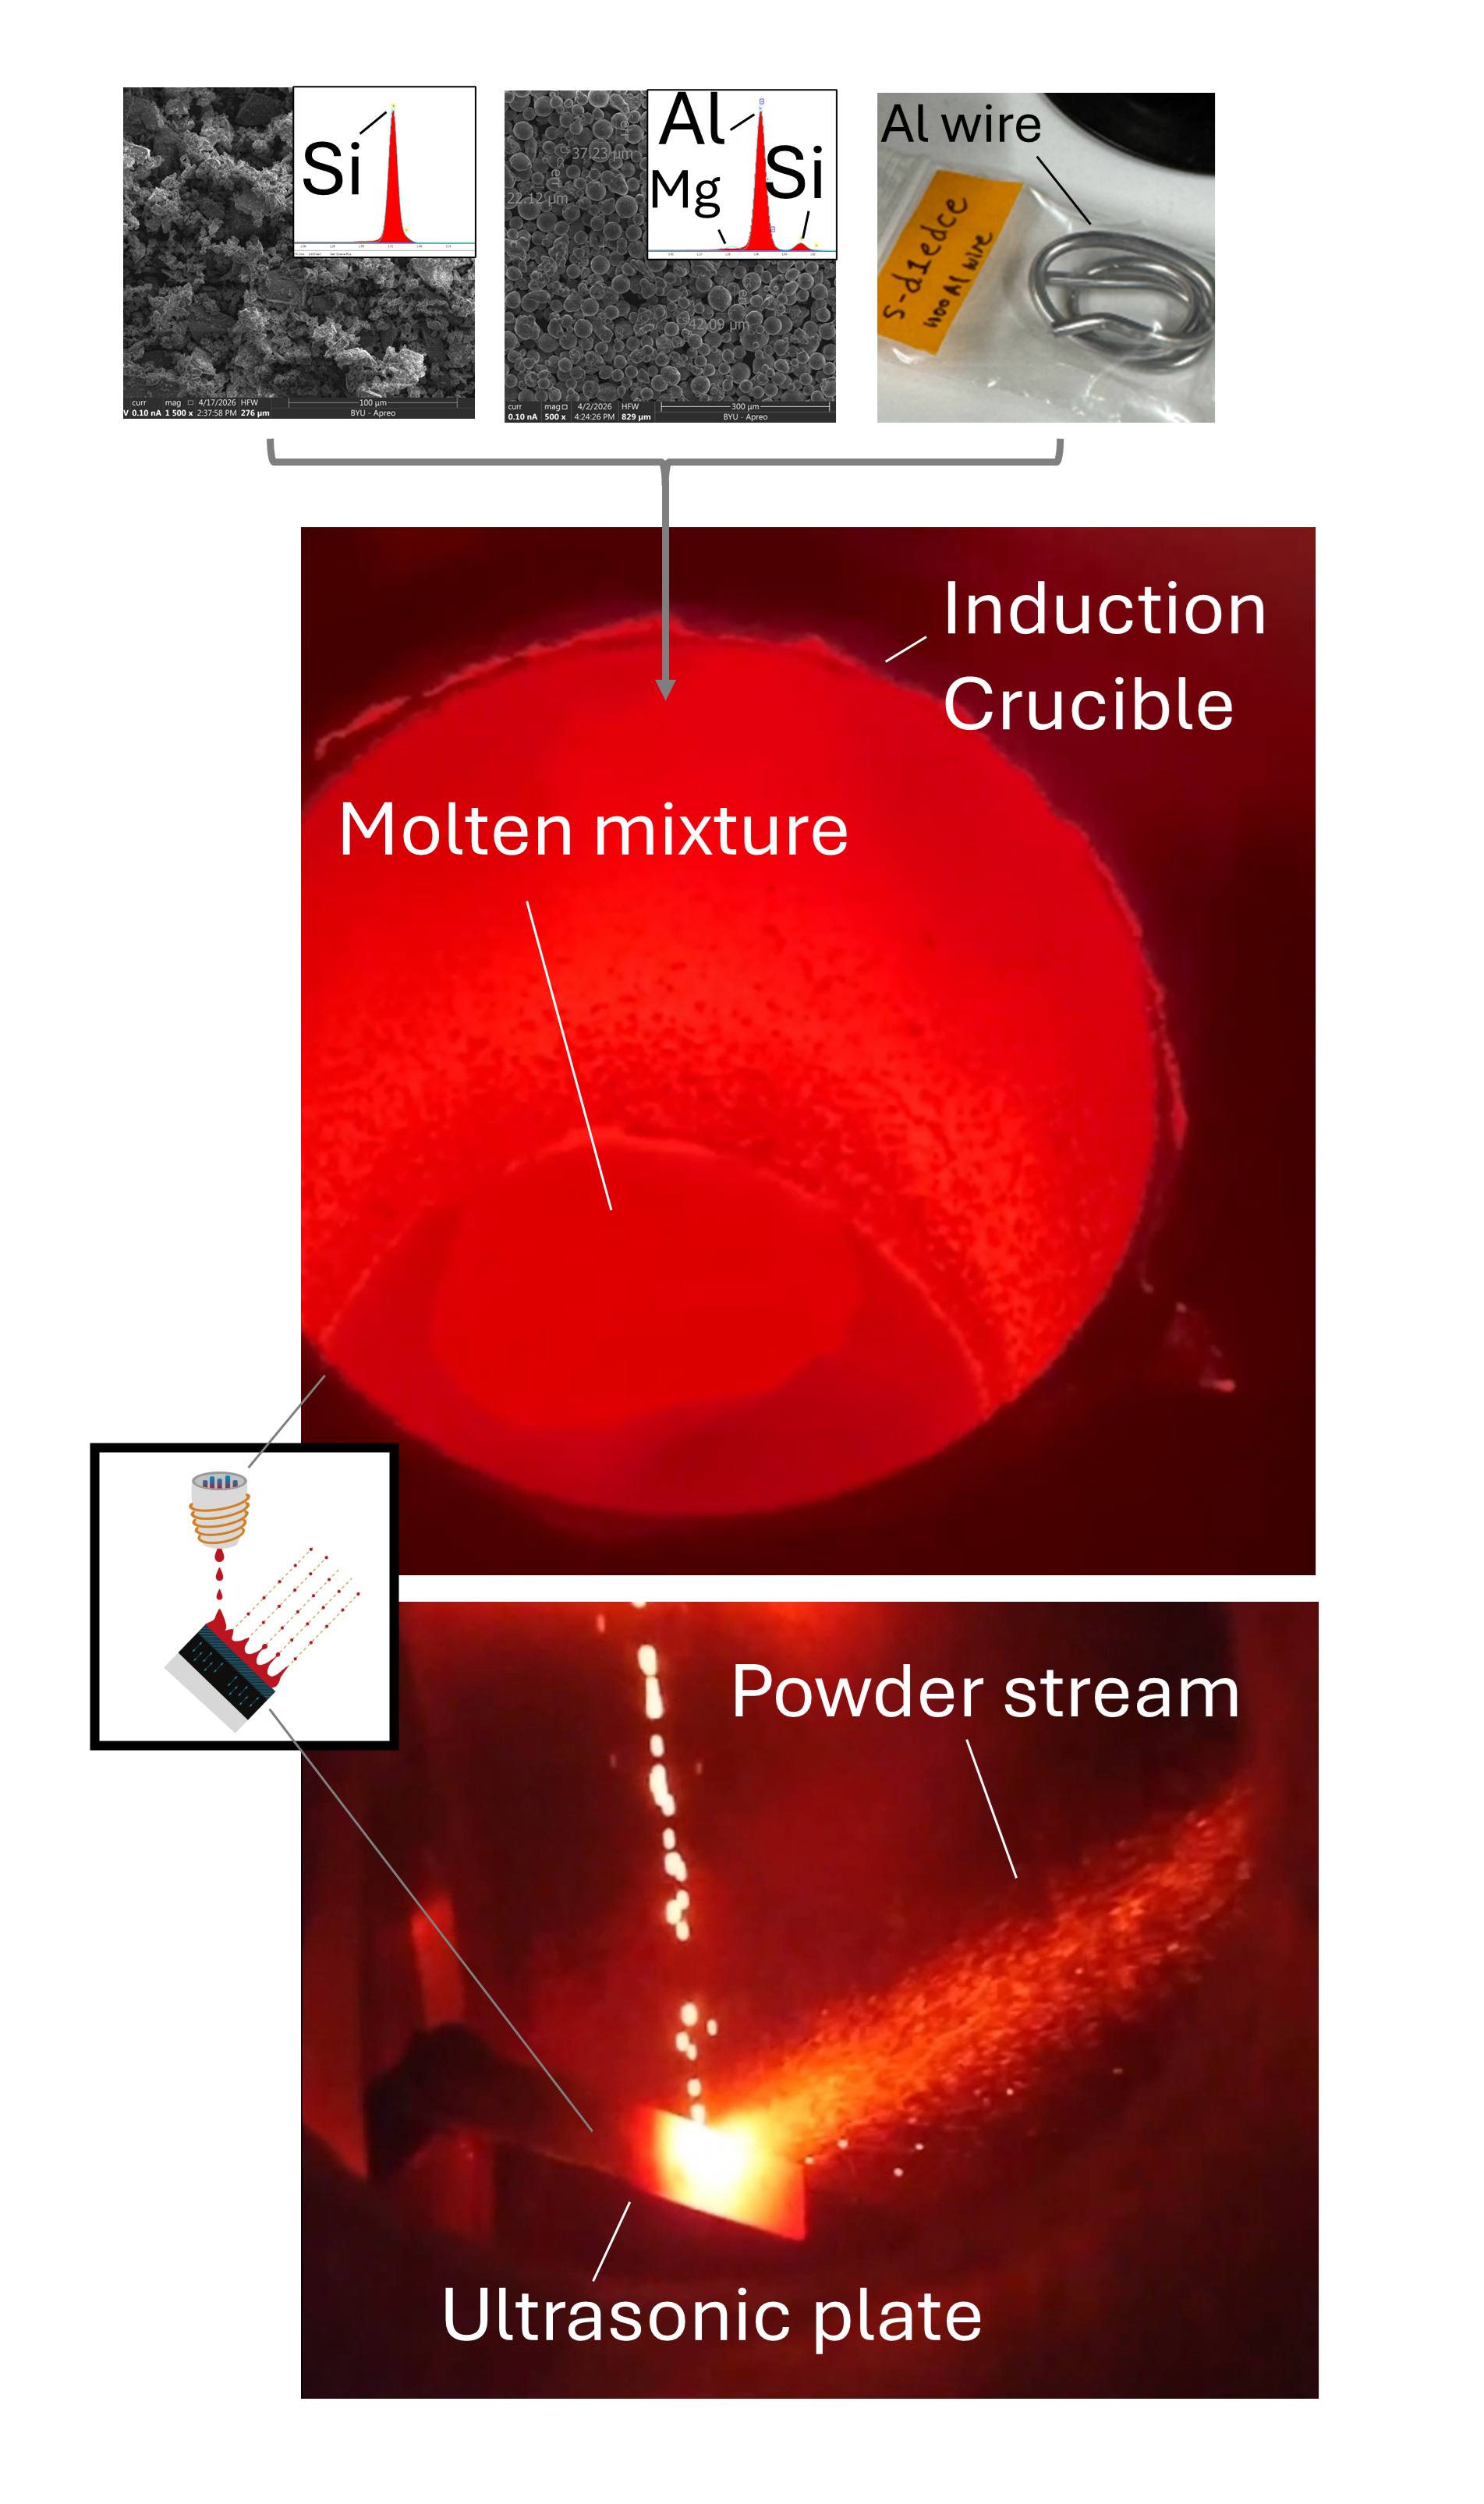
\includegraphics[width=\linewidth]{../genesis-mission-proposal/figures/atomization-process-annotated.png}
  \caption{\flaime{} atomization process: feedstock (Si + AlSi10Mg + 1100 Al wire, byu-vcl) $\to$ induction-crucible melt $\to$ ultrasonic-plate breakup (AMAZEMET rePOWDER).}
  \label{fig:baseline}
\end{wrapfigure}
The purpose of this proposal is to demonstrate how \flaime{} (Fast Learning AI for Mineral Efficiency) targets DOE Topic~3-B's critical mineral demand reduction
objective by closing the discovery~$\to$~manufacturing~$\to$~qualification
loop for \textbf{Sc-free, Mn-Cr-Zr-lean aluminum alloys for laser powder bed fusion (LPBF)}.%
\footnote{Buy America Act compliance: this project does not involve
construction, alteration, maintenance, or repair of public
infrastructure (FOA \S III.F).}
Manganese and zirconium are 100\% import-reliant and chromium 74\%
(USGS 2024~\cite{usgs_mcs_2024}). Scalmalloy is Sc-dominated, and the four
confirmed commercial Additive Manufacturing (AM) Al alloys (AlSi10Mg, Scalmalloy, AL250C,
AlSi7Mg)~\cite{wang_2024_ma171125,france_2019_scalmalloy,gradl_2022_s1166502,klippstein_2019_bracket,montanari_2023_met13040}
collectively concentrate U.S.\ AM production risk on these
elements, making it susceptible to a single supply chain disruption~\cite{bauer_2023_1998242}. We propose \flaime{}, a Level~3 self-driving laboratory
(SDL)\footnote{Level~3 in the taxonomy of Tom et
al.~\cite{tom_2024_acschemr}: a closed-loop, AI-guided platform in
which software selects experiments autonomously while a small set of
defined human handoffs execute physical transfers.}
that will discover LPBF aluminum alloys meeting structural
performance targets while minimizing critical mineral content.  Related
SDL/BO efforts include APEX~\cite{conn_2025_llnl_apex}, (DED, no LPBF/tensile)
A-Lab (oxides, not structural metals)
~\cite{szymanski_2023_s4158602}, AMASE (thin-film phase maps)
~\cite{liang_2025_sciadvad}, high-throughput DED active-learning without LPBF/tensile
qualification~\cite{nelaturu_2024_jmsea202};
BIRDSHOT (arc-melted refractories, pre-selected system)~\cite{paramore_2025_jactamat},
ICME-anchored closed-loop Al for AM~\cite{thapliyal_2020_jmtla201}, and BO-guided CALPHAD within a single expert-selected Al system~\cite{glaser_2025_jmps106120}. However, none
yet \emph{unify powder production, LPBF printing, and tensile testing
under a single AI decision loop with joint composition--process optimization}.  By closing this decision loop via a complete powder-to-part pipeline, \flaime{} targets a measurable
AI acceleration factor of $\geq$3$\times$ over conventional alloy
development for the decision making portion utilizing Bayesian
optimization. These estimates are consistent with
${>}$3--5$\times$ speedups reported for closed-loop materials campaigns\cite{liu_2024_llambo,paramore_2025_jactamat} and compounded with
closed-loop execution speedup from hardware and software automation for
an estimated ${\sim}$10$\times$ total reduction in discovery
time~\cite{tom_2024_acschemr}.

\textbf{Project relevance and context.}
The DOE Critical Materials Strategy (Pillars~2, 3, 5)~\cite{bauer_2023_1998242} and alloy level criticality metrics~\cite{titirici_2022_roadmap,graedel_2022_s4146702} motivate composition level supply risk optimization as a first-class Bayesian Optimization over Function Network (BOFN) objective alongside strength and printability. AMMTO's CMI Hub precedent (Al--Ce to TRL~9~\cite{lograsso_2024_2338076}) motivates the same urgency for lean critical mineral LPBF alternatives.  All confirmed commercial AM Al deployments (AlSi10Mg, Scalmalloy, AL250C, AlSi7Mg) use LPBF exclusively~\cite{wang_2024_ma171125,france_2019_scalmalloy,gradl_2022_s1166502,klippstein_2019_bracket,montanari_2023_met13040}, validating \flaime{}'s primary focus on LPBF.

\flaime{} bridges computation and physical qualification using \bofn{} minimizing mineral burden objective~\cite{astudillo_2019_icml,astudillo_2021_21121531}, building on
supply risk aware optimization~\cite{mulukutla_2024_ssrn4968}. Recent
cost-aware BO advances make AI guided powder-to-part discovery
tractable~\cite{chawla_2025_arxiv251116930}.

Several preliminary data have been collected specifically for this proposal to demonstrate feasibility and de-risk the proposed approach: powder characterization, mixing, and atomization of a custom blend, Thermo-Calc TCAl10/AM~Module CALPHAD simulations, LPBF printing, SEM/EDS characterization, and tensile tests for commercial AlSi10Mg powder, ~pKGFN~\cite{buathong_2023_23110214} optimization benchmarking campaigns using AM-like synthetic network functions running on BYU's HPC.
(Fig.~\ref{fig:pipeline}).

The Lead PI brings direct SDL experience since 2022 (incl. three years of Acceleration Consortium leadership) and lead authored the structural materials section in a comprehensive
SDL review~\cite{tom_2024_acschemr}, a frugal twin
framework~\cite{lo_2024_d3dd0022}, and a critical raw materials
article~\cite{titirici_2022_roadmap}. Prior high dimensional BO
work~\cite{baird_2022_commatsci,baird_2023_dib} informs \flaime{}'s
joint acquisition whose compositional subspace implicitly spans
\subsystemcount{} element combination subsystems. \textbf{Valimet brings significant expertise in gas atomization} and scaled up industrial atomization processes.

% --- 2. Project Objectives (~0.5 page) -------------------------------------
\section{Project Objectives}\pagebudget{0.5}
\label{sec:objectives}

% \guidance{FOA: ``Provide a clear and concise statement of the specific
% objectives of the proposed project.  Address how the objectives align
% with the chosen focus topic and lead to an AI advantage.''  Keep
% objectives quantitative, measurable, and few (3--5).}

% \guidance{COMMERCIALIZATION (Review Criterion 4, FOA p.85): ``Does the
% application articulate a credible strategy for technology transfer
% and/or commercialization beyond the project's duration?''  Since AMMTO
% is an applied technology office, include at least one objective or
% sentence addressing technology transfer path (e.g., software licensing,
% industry partnership, standards body engagement).}

\noindent\textbf{Goal.} Discover novel, high performing, critical mineral lean LPBF Al alloys for structural applications and demonstrate a
measurable \textbf{AI advantage} through established
metrics~\cite{tom_2024_acschemr}---specifically, AI acceleration factor, discovery yield, and mineral-burden reduction--- advancing the dual Topic~3B
mandate of AI enabled materials discovery \emph{and} reduced demand
for critical minerals.

\begin{enumerate}[label=\textbf{O\arabic*.},leftmargin=2em]
  \item Demonstrate a closed-loop BOFN/pKGFN platform for AI guided,
        cost-aware alloy exploration across the full powder-to-part pipeline.
  \item Cover a joint search space spanning \subsystemcount{} element
        combinations (Al + 15 alloying element upper bounds)
        and evaluate 100--200 compositions via CALPHAD partial evaluations
        under a mineral burden objective.
  \item Validate 100--200 compositions experimentally through the
        minimum viable specimen (MVS) pipeline over a 9-month Phase~I.
  \item Achieve discovery yield $\geq$3\%
        % (3--6 alloys meeting family specific mechanical thresholds
        \emph{and} satisfy the
        dual baseline Gate~G3 mineral burden constraints vs.\ Scalmalloy
        and AlSi10Mg.
  \item Demonstrate AI acceleration factor~\cite{tom_2024_acschemr}
        $\geq$3$\times$ vs.\ a pre-registered random
        baseline~\cite{sabanzagil_2025_s4358802}, with bootstrap CIs
        across $\geq$20 seeds.
\end{enumerate}

\noindent Per-family YS/EL thresholds, the Tier~1 pass-rate complementary
metric, and throughput derivation are given in and
App.~\ref{app:facilities}.

\noindent Collectively, fulfillment of these objectives demonstrate that a
software orchestrated, AI guided closed-loop platform can
simultaneously accelerate alloy discovery \emph{and} reduce critical
mineral dependence---the dual mandate of Topic~3B. Phase~I focuses on
Al alloys processed by LPBF.
Al with the \elementcount-element palette (\elementlisttex{}) span 0\%
to 100\% USGS import reliance, ensuring the mineral burden objective
produces genuine supply risk tradeoffs.

\textbf{Technology transfer and commercialization.}  All \flaime{}
software releases open source (permissive licensing) via BoTorch tutorials~\cite{balandat_2019_19100640} per Meta's letter of collaboration and Honegumi~\cite{baird_2025_honegumi}. Discovered
alloys will be published openly rather than licensed: the most broadly
adopted AM Al alloy (AlSi10Mg) is unpatented, and even
patented high-performers (e.g., Scalmalloy) reached broad adoption
primarily through standardization and industry partnerships.
The team has prepared an extensive \textbf{multi-site validation network of collaborating universities,
national labs, and companies} that
have agreed to accept a batch of gas-atomized powder for one or more  \flaime{} alloy compositions, print a specimen on their metal 3D printer (LPBF/DED/Binder Jet), and return a printed sample with associated build metadata so that alloy performance can be cross-validated across printers and process conditions rather than localized to a single machine (Fig.~\ref{fig:flaime-dag}); each partner site contributes in-kind printer/operator
time with potential for further collaborations in a Phase~II continuation.  The team will also submit several presentations to SME's RAPID~+~TCT~2027 (largest North-American AM conference, April~2027) and pursue a complimentary academic booth showcasing \flaime{} software, tutorials, and validated compositions---just outside the Phase~I period of performance which ends 31~March~2027 and therefore not charged to this award.

% --- 3. Proposed Research and Methods (~1.5 pages) --------------------------
\section{Proposed Research and Methods}\pagebudget{1.5}
\label{sec:methods}

\guidance{FOA: ``Provide a clear research plan for a 9-month project
and describe the proposed activities and methods.  Include enough
technical details to evaluate the impact of the proposed activity.  For
each activity, indicate the responsibility of the key investigator(s)
and the associated budget.  If building on existing DOE-funded work,
describe how this is distinct.''}

\instruct{This is the center of gravity.  Must cover:
(1) AI framework (\bofn{} DAG or equivalent),
(2) experimental pipeline (powder $\to$ print $\to$ test),
(3) closed-loop integration,
(4) qualification-relevant data generation.
Include a system architecture figure if it fits within the 5-page
limit --- otherwise move it to an appendix reference or describe
textually.  Tables and figures count against the limit, so use them
very selectively.}

\guidance{FY27 GO/NO-GO CONTINUATION (FOA p.57; FAQ 4/15/2026): FY26
Focus Area 3-B does not accept Phase II applications in FY26; however,
all FY26 Phase I awards undergo a go/no-go review no earlier than
6~months after award start for eligibility to apply to a future
continuation solicitation (scope and focus-area set TBD, subject to
appropriations).  Frame Phase~I as demonstrating readiness for
3x--5x scale-up and for generalization from the demonstration alloy
system to AMMTO's core materials portfolio (e.g., 316H, IN718,
Hastelloy N), positioning the team for FY27 go/no-go continuation
eligibility.}

\guidance{FULL PIPELINE DESCRIPTION (FOA p.70): ``Applications should
describe the full pipeline of data generation and curation; experiments
and observation, AI model training, fine tuning, and inferencing; and
integration, using agentic techniques or otherwise, into a capability
of use for science or engineering.''  Ensure all pipeline stages are
explicitly addressed.}

\guidance{TEAM COORDINATION (Review Criterion 3, FOA p.84): ``To what
extent does the application demonstrate a clear, well-coordinated
collaboration among partnering institutions, with appropriately balanced
responsibilities, synergistic contributions, and clearly defined roles
for each team member?''  Address communication cadence, data handoff
protocols, and decision-making structure.}

\textbf{Activity~1: AI-Guided Computational Exploration}
(\emph{PI, BYU {$\sim$}\$220K}).

The \flaime{} optimizer is a \bofn{} directed acyclic graph
(DAG; Fig.~\ref{fig:flaime-dag})~\cite{sundar_2025_s4357802,paramore_2025_jactamat} covering
Thermo-Calc AM~Module simulation, powder, LPBF, and mechanical response nodes.
The \emph{partial} Knowledge Gradient for Function
Networks (pKGFN)~\cite{buathong_2023_23110214,buathong_2025_25061145}
is the acquisition function that selects which node and inputs to
evaluate next in a cost-aware manner: ``partial'' because not every
node is evaluated at each iteration (e.g., a Thermo-Calc AM~Module
query can be run without triggering an expensive tensile test),
``knowledge gradient'' because the decision model maximizes the expected
improvement in the global objective per unit cost
ranging from Thermo-Calc AM~Module simulation to tensile testing, and
``network'' because the DAG structure---where each node's output feeds downstream nodes---is exploited to propagate information efficiently (Fig.~\ref{fig:pipeline}).
A mineral burden node (analytical, noise-free) exposes two cost-weighted
scalars to act as hard supply chain metrics: $\mathrm{MBS}_{\text{lin}}{=}\sum_{i\neq\mathrm{Al}}\mathrm{NIR}_i(c_i/c_{\mathrm{Al}})x_i$
as a gate (G3a) on Sc-elimination and $\mathrm{CMDRI}_{\text{log}}{=}\sum_{i\neq\mathrm{Al}}\mathrm{NIR}_i\log_{10}(1+c_i/c_{\mathrm{Al}})x_i$
for continuous BOFN objective and a gate (G3b) for backfill ceiling vs.\ AlSi10Mg, see
Table~\ref{tab:gates}. USGS MCS~2024 NIR~\cite{usgs_mcs_2024}
and 2022--2024 prices frozen at month 1
% (2025 USGS list adds Al/Si/Cu; base Al excluded)
will be used. Graedel~\cite{graedel_2012_es203534}, Helbig~\cite{mulukutla_2024_ssrn4968},
ESSENZ~\cite{cimprich_2019_jiec1286}, and $\mathrm{HHI}_{\text{prod/res}}$
enter as digital-thread reporting metadata/contextual BOFN features instead of hard thresholds % (not gate multipliers)
per the multi-axis framework of Baird~\&~Sparks~\cite{titirici_2022_roadmap}. Preliminary pKGFN benchmarking campaigns on BYU's HPC and preliminary CALPHAD and AM Module evaluations have been performed.

\begin{wrapfigure}{r}{0.55\linewidth}
  \centering
  \vspace{-\intextsep}
  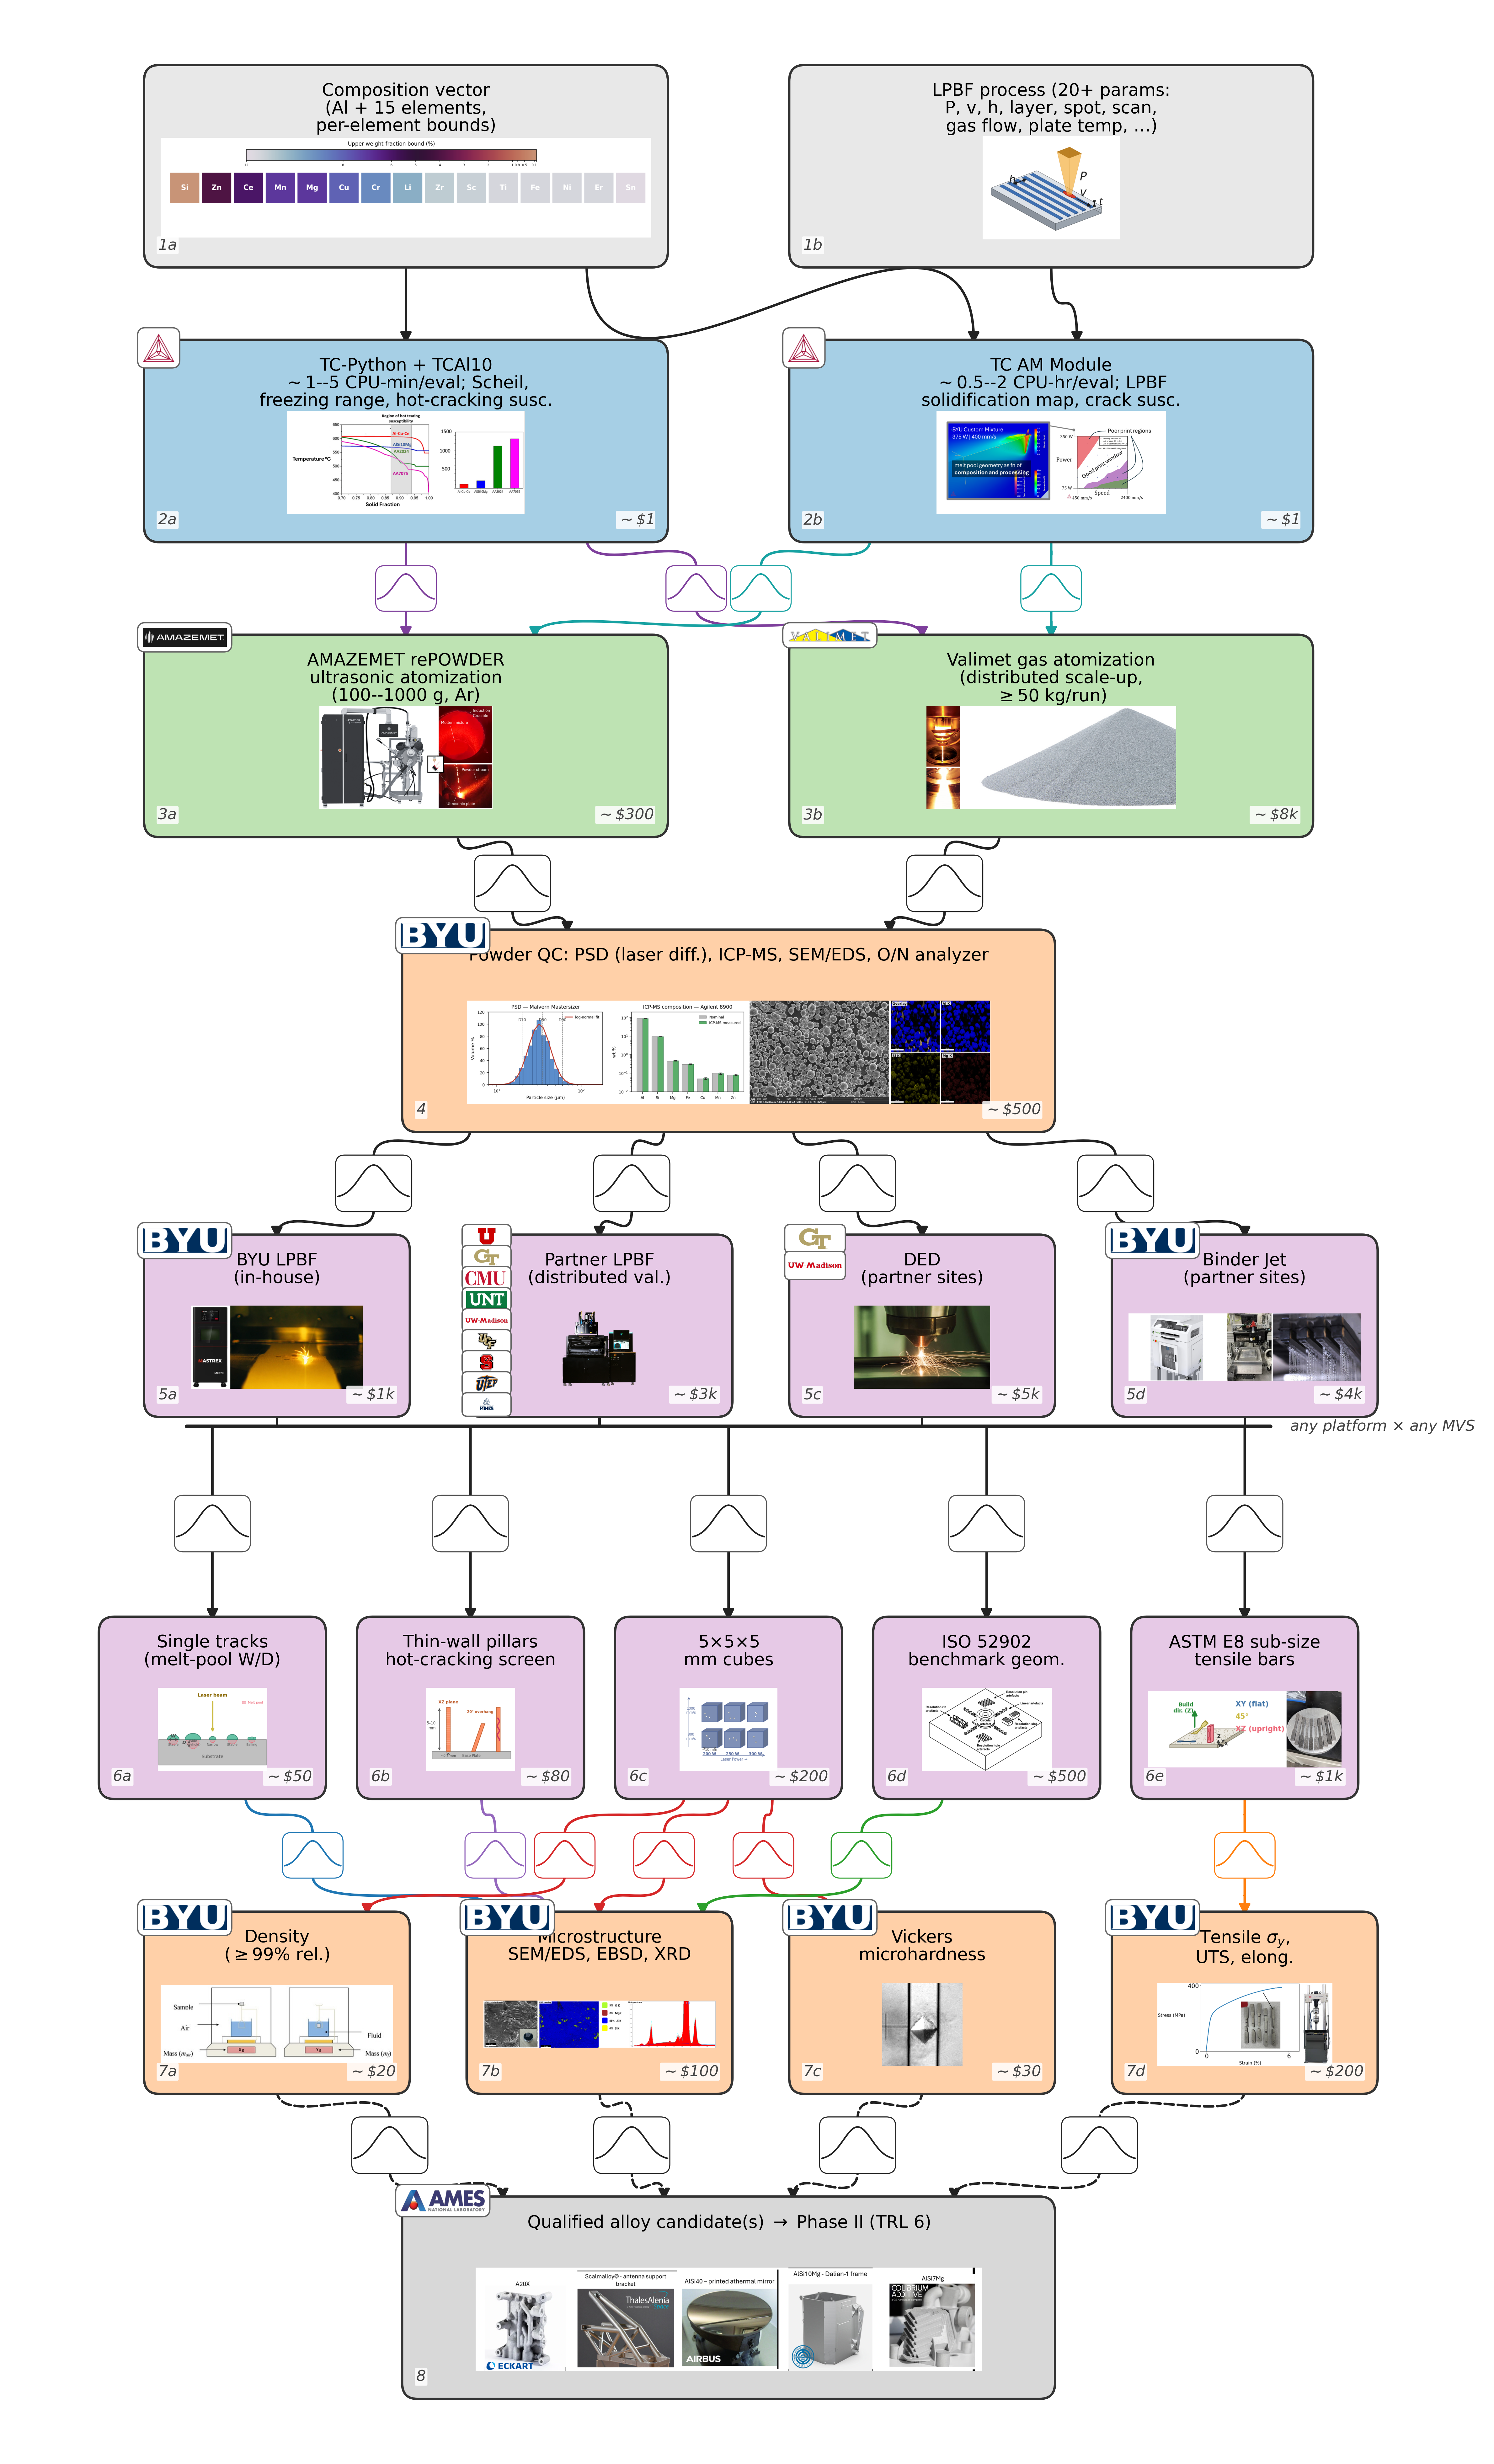
\includegraphics[width=\linewidth]{../figures/flaime_pipeline_dag.png}
  \caption{\flaime{}'s Bayesian Optimization Function Network (BOFN) for AM alloy discovery.}
  % Long-form caption commented out for brevity; restore if page budget allows.
  % \caption{\flaime{} BOFN pKGFN acquisition DAG (top$\to$bottom): joint composition + LPBF process inputs $\to$ parallel CALPHAD partial-evaluation nodes (TC-Python/TCAl10, AM~Module) $\to$ \textbf{atomization siblings} (rePOWDER ultrasonic $\sim$\$300/run vs.\ Valimet gas atomization; categorical fidelity dimension) $\to$ shared powder QC $\to$ \textbf{AM platform siblings} (BYU LPBF / Partner LPBF / DED / Binder Jet, $\sim$\$1--5k/build; second categorical fidelity dimension routed through the horizontal bus) $\to$ shared MVS ladder (single tracks, thin-wall pillars, cubes, ISO~52902, ASTM~E8) $\to$ density/microstructure/hardness/tensile $\to$ Phase~II commit (dashed). In-node thumbnails are representative artifacts/results from each pipeline stage (placeholders shown where final imagery is pending); top-left corner badges identify the partner asset associated with each node. Any (powder source $\times$ AM platform) combination is admissible to pKGFN; cost-aware acquisition selects expensive combinations (Valimet, DED, Binder Jet, ASTM~E8 bars) sparingly and cheap combinations (rePOWDER + BYU LPBF + single tracks) densely. Per-node $\sim$\$X chips are approximate per-evaluation costs that drive the cost-aware acquisition. Per BOFN/pKGFN~\cite{buathong_2023_23110214,buathong_2025_25061145} every internal node has its own GP surrogate; the bell-curve glyph on each node-to-node edge denotes forwarding of the upstream node's GP posterior $p(y_k\,|\,\mathcal{D}_n)$ as a structured input to the downstream surrogate; colored edges encode the routing source (purple/teal from TC nodes to atomization siblings; per-MVS color from MVS to characterization). Only the root composition/process inputs feed CALPHAD without a glyph because they are not GP-modeled. Bottom-left corner labels (1a, 1b, \ldots, 8) provide stable node identifiers for cross-references in the narrative, captions, and risk register.}
  \label{fig:flaime-dag}
\end{wrapfigure}

\begin{figure}[p]
  \centering
  \includegraphics[width=0.85\linewidth]{../benchmarks/figures/actions_full/pKGFN.png}
  \caption{Optimization performance comparing between pKGFN and other benchmarks demonstrating superior cost-efficiency through partial evaluations of a complex manufacturing problem \cite{buathong_2023_23110214}, similar to the complex multi-step AM alloy discovery pipeline proposed here.}
  \label{fig:pipeline}
\end{figure}

\textbf{Joint Acquisition with GA Inner Solver.}
The 15 alloying element palette upper bounds (Al + \elementlisttex{})
define the outer feasibility envelope, baseline family priors and USGS-derived mineral burden. The live pKGFN BO loop in
Phase~I jointly optimizes the \textbf{full 15-element bounded composition
vector and 20+ additional synthesis and processing variables across the powder-to-part pipeline} under a single asynchronous, cost-aware acquisition. Sparse Axis Aligned Subspace Bayesian Optimization (SAASBO), shown to work well in high dimensions \cite{eriksson_2021_21030034,baird_2022_commatsci}, will be used as the node-specific surrogate model for the downstream experimental nodes (highest fidelity, highest cost). A genetic algorithm will be used to solve the non-differentiable acquisition inner loop without resorting to pre-enumerating the candidate search space.
The full compositional outer envelope implicitly spans
$\sum_{k=2}^{8}\binom{\elementcount}{k}=\subsystemcount{}$
element combination subsystems (\feasiblepairsOneAt{} strictly
supported compositions at 1\,at.\% resolution; \feasiblepairsTenthWt{}
at 0.1\,wt.\%, Al\,$\geq$\,85\,wt.\%).
Pending evaluations are handled via fantasy samples (model predictions of pending points fed back into the model temporarily) so the acquisition
stays asynchronous across simulation and experimental queues. The campaign will begin with several baselines followed by a set of 32 Sobol quasi-random designs to kickstart the campaign with space-filling
initial points before pKGFN takes over. 
% \emph{CALPHAD partial-evaluation nodes.}
% \texttt{pycalphad}~\cite{otis_2024_97810035}
% $\sim$ms--sec/eval; license-free batch evaluation of phase fractions and CSI as contextual features),
TC-Python + TCAl10 Scheil + TC-PRISMA % ($\sim$1--5\,CPU-min/eval)
and the Thermo-Calc AM~Module % ($\sim$0.5--2\,CPU-hr/eval; printability, melt-pool)
sit as three parallel cheap-to-costly contextual nodes to serve as inputs
that inform the surrogate but are not themselves tunable decision
variables. pKGFN chooses per candidate which to query under the cost
budget. The use of \texttt{pycalphad}~\cite{otis_2024_97810035} with open-source databases will be explored; however, the databases are much . AM~Module predictions map to Aconity MIDI parameters and are
reciprocally calibrated by FLAIME prints. In line with the aims of Topic 3B, a mineral burden score is treated as a
first-class BOFN objective~\cite{bocklund_2020_20011161,eriksson_2021_21030034,sabanzagil_2025_s4358802}.
Mineral lean family caps Mn\,$\leq$\,0.5, Cr\,$\leq$\,0.3,
Zr\,$\leq$\,0.5, Sc\,$\leq$\,0.05\,wt.\% with gate G3b as the primary
discovery constraint. Al--Mn--Cr--Zr~\cite{thapliyal_2020_jmtla201} % (lightweight high-strength LPBF)
and Al--Zr % (L1$_2$ precipitate strengthening, thermal stability)
serve as performance baseline comparators: both atomized early to seed the surrogate, ground the
mineral burden benchmark, and validate the pipeline before committing
the full campaign budget. A pre-registered pKGFN vs. standard BO
ablation plan will be developed within the first two months of the project.

\textbf{Activity~2: Powder $\to$ Print $\to$ Test Pipeline}
(\emph{PI + partners; BYU {$\sim$}\$280K, plus the Valimet subaward}).
%
Powder feedstocks are produced via ultrasonic atomization using AMAZEMET
rePOWDER, en-route from Poland as of 2026-04-24, for rapid
composition iteration---mixtures of elemental powders are dosed at
0.1\,mg resolution---providing high
compositional design freedom.
\textbf{Valimet (funded subrecipient) provides significant
intellectual leadership} as co-developer of the
gas-atomization scale-up envelope: joint definition of process windows
for $\sim$6 production scale runs at $\geq$50\,kg, joint specification
of powder acceptance criteria (PSD, oxygen, ICP, satellites/morphology) and contribution to the manufacturability gates that feed back into the
BOFN loop. The deliverable will be the 6 scale-up runs plus the additional shared design of the scale-up envelope and the
specifications under which BYU ultrasonic-atomized screening
compositions are deemed transferable to commercial gas atomization.
Inductively coupled plasma mass spectrometry (ICP-MS) using BYU's Agilent~8900 provides authoritative bulk-composition
verification against design target. Scanning Electron Microscopy combined with Energy Dispersive Spectroscopy (SEM/EDS) (Fig.~\ref{fig:baseline})
maps particle spatial distribution and is benchmarked against
ICP-MS per the provenance audit. This will be done every $k{=}10^{\text{th}}$ composition with
$>$5\% relative EDS--ICP-MS disagreement triggering a re-run. Initial
validation test mixtures composed of AlSi10Mg+Si+Al-wire have been
atomized in advance through pre-collaboration with AMAZEMET.
LPBF printing is performed at University of Utah's Multiscale Mechanics \& Materials Lab led by Dr. Ashley Spear. Specimens follow a
minimum-viable ladder (single tracks $\to$ thin-wall pillars $\to$
density cubes $\to$ ASTM~E8/E8M sub-size tensile bars), with each stage
gating the next on a partial evaluation of cost awareness and any stage
early-stoppable. It creates a staged funnel: $\sim$160 atomized $\to$ $\sim$80 LPBF
density cubes
% ($\geq$99\% relative density gate)
$\to$ $\sim$40 ASTM~E8
tensile $\to$ top-3 elevated-temperature validation
(Appendix~8 \S A8.3).
Sub-size ASTM~E8/E8M (100\,mm) specimens are standard for LPBF
screening~\cite{paraschiv_2023_ma16144930,wang_2020_17452759}.
Preliminary AlSi10Mg results validate the pipeline. An initial specific
composition (Mehta ``Alloy~C'':
Al--5.0\,wt.\%\,Mn--0.8\,wt.\%\,Cr--0.5\,wt.\%\,Zr) has been sent to
Thermo-Calc for AM~Module evaluation.

\textbf{Activity~3: Closed-Loop Integration, Dissemination \&
Qualification} (\emph{PI, BYU; {$\sim$}\$100K}).
%
The pKGFN engine orchestrates autonomous cycles: GP surrogates retrain
after each batch and select next compositions and parameters and
dispatched operating procedures map human handoffs 1:1 to future robotic
points, minimizing technical debt. ISO~52902 benchmark geometries are
printed as a BOFN node throughout the campaign, providing relevant parameter and qualification data stored with MongoDB. Data will be FAIR released to
Zenodo/Figshare and AmSC-hosted Genesis Mission integration (App.~4 DMSP).

\textbf{Project Management, Risk \& Prior Work.}
Weekly PI--partner calls will be hosted. A FAIR-compliant database will be used as a single source of
truth. Two Master students alongside about four full-time and four part-time undergraduate students in six-day/week shifts will form the lab staff to produce up to
16~compositions/week per Gantt, see Appendix~2. A compact risk register is given in Appendix~7 (\S A7.0).
\flaime{} builds on the PI's Honegumi SDL infrastructure and Fehrmann
Materials ML-guided alloy contract but represents new closed-loop integration of composition discovery with AM qualification---no prior DOE funding supports this work.

% --- 4. Milestones in the Nine Months (~1 page) ----------------------------
\section{Milestones in the Nine Months}\pagebudget{1}
\label{sec:milestones}

\guidance{FOA: ``Provide a list of clearly defined and measurable
milestones of the project.''  These should be concrete deliverables, not
activities.  Include Go/No-Go decision gates.}

\begin{table}[H]
\centering\footnotesize
\caption{Phase~I milestones and deliverables (9~months).}
\label{tab:milestones}
\setlength{\tabcolsep}{3pt}
\begin{tabularx}{\textwidth}{clX}
\toprule
\textbf{Mo.} & \textbf{ID} & \textbf{Milestone / Deliverable} \\
\midrule
1 & M1 & BOFN DAG deployed; pKGFN joint acquisition with GA inner solver live on BYU HPC; CALPHAD partial-evaluation nodes (pycalphad, TCAl10, AM~Module) queried across the 15-element palette; first experimental batch selected by the joint acquisition; Al--Mn--Cr--Zr and Al--Zr baseline-comparator atomization runs initiated to seed the surrogate and ground the mineral-burden benchmark \\
2 & M2 & $\geq$10~cumulative atomization runs (baselines + Sobol) pre-seed the surrogate; powders characterized by particle size distribution (PSD), SEM/EDS and ICP-MS; pre-registered 5-baseline benchmark frozen; \textbf{powder-transfer validation:} Al--Mn--Cr--Zr ``Alloy~C'' produced by both AMAZEMET ultrasonic and Valimet gas atomization with PSD/chemistry/oxide/density-window/tensile compared (PSD D50 $\pm$15\%, O $\pm$30\%, density-window overlap $\geq$70\% gates whether ultrasonic data substitutes for gas-atomized scale-up; if poor, branch to ultrasonic-only Phase~I closure with explicit gas-atomized Phase~II handoff) \\
3 & M3/G1 & \textbf{Go/No-Go G1:} $\geq$50 compositions evaluated under joint pKGFN acquisition; GP surrogate RMSE $<$ pre-registered threshold (nested CV). \textit{If fail: retrain with augmented CALPHAD; +1~month.} \\
5 & M4/G2 & \textbf{Go/No-Go G2:} $\geq$1 complete AI orchestrated CALPHAD$\to$atomization$\to$LPBF$\to$tensile$\to$BOFN cycle demonstrated end-to-end; $\geq$2 compositions at $\geq$99.5\% relative density. \textit{If fail: decouple pipeline; run stages independently with manual scheduling.} \\
7 & M5/G3 & \textbf{Go/No-Go G3:} $\geq$1 alloy meeting family thresholds (Al-Mn-Cr-Zr: YS$\geq$250~MPa, EL$\geq$5\%; Al-Zr: YS$\geq$200~MPa, EL$\geq$8\%), or $\geq$1 AI discovered alloy outside the baseline families at equivalent thresholds; G3a $\mathrm{MBS}_\text{lin}\leq$10\% of Scalmalloy \emph{and} G3b $\mathrm{CMDRI}_\text{log}\leq$1.5$\times$ AlSi10Mg; ASTM~E8 sub-size, $\geq$3 replicates. \textit{If fail: pivot to strongest partial-pass; intensify BOFN exploitation.} \\
9 & M6 & Final deliverables: digital thread ($\geq$85\% completeness with supply-risk metadata); dual-gate CMDRI validation and 2D DoE-style criticality matrix (NIR vs.\ $\mathrm{HHI}_\text{production}$) reporting; pre-registered AI benchmark report (AF, win rate, bootstrap CI); FY27 continuation readiness assessment (per FOA go/no-go) \\
\bottomrule
\end{tabularx}
\end{table}

\instruct{Milestones must be clearly defined and measurable --- not just
``continue work on X.''  Each Go/No-Go gate should have a quantitative
pass/fail criterion.  Example: G1 = AI model trained on $\geq$50
compositions with RMSE $<$ threshold; G2 = closed-loop cycle
demonstrated end-to-end; G3 = $\geq$1 alloy meeting target properties.}

\guidance{6-MONTH DOE REVIEW POINT (FOA p.61): ``go/no go evaluation at
6 months.''  Structure the milestone table around this checkpoint --- the
month 5--7 Go/No-Go gates are the primary decision point for DOE
program managers.  The final 9-month milestones confirm completion but
the 6-month review determines continuation.}

% --- 5. Data Sources and Models (~0.5 page) --------------------------------
\section{Data Sources and Models}\pagebudget{0.5}
\label{sec:data}

\guidance{FOA: ``Describe which existing or new data sources will be
used.  Address your team's access to the data.  If applicable, indicate
which AI models or frameworks will be used.  Do NOT include computing
resource descriptions here --- that goes in Appendix 2 (Facilities).''}

\textbf{Data sources.}
CALPHAD: Thermo-Calc TCAl10 (Al)/TCMG6 (Mg) via TC-Python under BYU's HPC license (Thermo-Calc letter, App.~7). DFT energies from Materials Project~\cite{jain_2016_14944683} and AFLOW~\cite{oses_2018_18030503} via Matminer~\cite{ward_2018_jcommats}; experimental benchmarks: MMPDS, Knovel, ASM Alloy Center. Supply-risk scoring uses USGS MCS~\cite{usgs_mcs_2024} and DOE Critical Materials Assessment~\cite{bauer_2023_1998242}; BO integration follows~\cite{mulukutla_2024_ssrn4968}. These databases are used primarily to seed initial trials: literature-reported compositions are reproduced one-to-one as bias-free in-house ultrasonic-atomization replicates so all subsequent BOFN evaluations share a common feedstock-and-process baseline. \flaime{}-generated data publish to Zenodo/Figshare with DOIs.

\textbf{AI models.}
\bofn{} with pKGFN acquisition drives cost-aware selection atop GPyTorch/BoTorch GP surrogates~\cite{balandat_2019_19100640}, released open-source as Honegumi/BoTorch tutorials (Meta letter, App.~7). \flaime{} hosts its digital thread on AmSC as a plug-and-play GM capability and leverages other GM teams' characterization data to accelerate surrogate training (App.~4 DMSP).

% --- 6. Decision Gate Metrics (~0.5 page) -----------------------------------
\section{Decision Gate Metrics}\pagebudget{0.5}
\label{sec:gates}

\guidance{FOA: ``Provide specific metrics that can be used for the
evaluation of Phase I go/no go decision.  DOE encourages the development
of metrics to identify AI advantage.  One such metric could include
scaling behavior which shows increasing performance as additional data,
computing, and/or other resources are applied.  Quantitative statements
enabling transformative science and engineering through AI are
preferred.''}

\instruct{Key metrics to define: (1) AI advantage metric (e.g.,
compositions screened per unit time vs.\ conventional), (2) scaling
behavior (does performance improve with more data/compute?), (3)
qualification-relevant metric (how much of the traditional qualification
process is compressed?).  All metrics must be quantitative.}

\guidance{SCALABILITY (Review Criterion 2, FOA p.84): ``Does the
application address potential scalability issues?''  Include at least
one metric demonstrating scaling behavior --- e.g., compositions
screened per week as dataset grows, or model accuracy as function of
training data volume.  AMMTO values paths from lab-scale to
production-scale.}

\guidance{AI ADVANTAGE --- define precisely what ``AI advantage'' means
for this project: (1)~10x faster screening (5 days/composition vs.\
8--32 weeks conventional), (2)~autonomous experimental campaigns that
reduce human labor per composition, (3)~compressed qualification
timelines via digital thread.  The FOA uses ``AI advantage'' as a
central evaluation concept; your Decision Gate Metrics must quantify it.}

\noindent Three pre-registered Phase~I gates quantify AI advantage: \textbf{(1)~AI Acceleration Factor (AF)}---$\mathrm{AF}(y)=n_{\mathrm{baseline}}/n_{\mathrm{BOFN}}$ vs.\ four pre-registered baselines (random, expert DOE, standard BO, \bofn{} ablation w/o mineral-burden). Algorithms will be benchmarked against $\geq$20 seeds with bootstrap CI~\cite{sabanzagil_2025_s4358802}. The desired \emph{target factor}~$\geq$3$\times$ vs.\ random. \textbf{(2)~Discovery Yield}---fraction of BOFN-proposed compositions meeting family thresholds (Al-Mn-Cr-Zr: YS\,$\geq$\,250\,MPa, EL\,$\geq$\,5\%; ASTM~E8 sub-size) and supply-risk reduction vs.\ Scalmalloy with a desired \emph{target}~$\geq$\,3\%. \textbf{(3)~Mineral-Burden Reduction (dual G3)}---G3a $\mathrm{MBS}_\text{lin}\leq 0.10{\times}$Scalmalloy (Sc-elimination) \emph{and} G3b $\mathrm{CMDRI}_\text{log}\leq 1.5{\times}$AlSi10Mg. All formulas, caps, and thresholds are in App.~8 \S A8.1/\S A8.4. M6 will include a report with 2D NIR vs.\ $\mathrm{HHI}_\text{prod}$ matrix~\cite{titirici_2022_roadmap}. The desired \emph{target} is to pass G3a \& G3b. \textbf{Scaling \& AI:} To measure model effectiveness, model diagnostics are tracked every 25~compositions. Edison and Copilot will aid in drafting with all AI output reviewed.

% ============================================================================
%  APPENDIX 1: BIBLIOGRAPHY & REFERENCES CITED
%  (Does NOT count against 5-page narrative limit)
% ============================================================================
\newpage
\pagenumbering{roman}\setcounter{page}{1}% Reset page numbering at appendices so narrative is unambiguously 5 pages.
\section*{Appendix 1: Bibliography \& References Cited}
\label{app:references}

\required{FOA \S IV.C: ``Provide a bibliography of any references cited
in the Project Narrative.  Each reference must include the names of all
authors (in the same sequence in which they appear in the publication),
the article and journal title, book title, volume number, page numbers,
and year of publication.'' No page limit for this appendix.}

% Include refs that appear in the bibliography but are not yet \cite'd inline.
% These were in the original hand-written list; add inline \cite's as the
% narrative is expanded.
\nocite{abolhasani_2023_s4416002}  % [old 1]  Abolhasani & Kumacheva, Nat. Synth. 2023
\nocite{stach_2021_jmatt202}       % [old 2]  Stach et al., Matter 2021
\nocite{buathong_2023_23110214}    % [old 6]  Buathong et al., partial evaluations 2023
\nocite{khatamsaz_2023_s4152402}   % [old 7]  Khatamsaz et al., npj Comp. Mat. 2023
\nocite{liang_2025_sciadvad}       % [old 8]  Liang et al., Science Advances 2025
\nocite{bukkapatnam_2023_24725854} % [old 9]  Bukkapatnam, IISE Trans. 2023
\nocite{isoastm_52902_2023}        % [old 16] ISO/ASTM 52902:2023
\nocite{isoastm_52907_2019}        % [old 18] ISO/ASTM 52907:2019

\instruct{Must cite inline (currently only \textbackslash nocite'd):
Abolhasani \& Kumacheva 2023 (Nat.\ Synth.),
Stach et al.\ 2021 (Matter),
Khatamsaz et al.\ 2023 (npj Comput.\ Mater.),
Liang et al.\ 2025 (Sci.\ Adv.).}

\renewcommand{\bibsection}{}% suppress auto-generated "References" heading
\bibliographystyle{unsrtnat}
\bibliography{edison-references}

% ============================================================================
%  APPENDIX 2: FACILITIES & OTHER RESOURCES
%  (0.5 page max; does NOT count against narrative limit)
% ============================================================================
\newpage
\section*{Appendix 2: Facilities \& Other Resources}
\label{app:facilities}

\required{FOA \S IV.C: ``Identify the resources and/or facilities to be
used. If appropriate, indicate their capacities, pertinent capabilities,
relative proximity, and extent of availability to the project. Describe
only those resources that are directly applicable to the proposed work.
Describe the computing, networking, and data resources required.''
Maximum 1 page.}

\instruct{Describe: (1) BYU lab --- atomizer, SEM/EDS, tensile tester;
(2) partner LPBF access --- machine specs, access agreement; (3) national
lab facilities if applicable; (4) computing resources (cluster, cloud,
potential DOE HPC allocation).  Frame as leveraging existing DOE-funded
infrastructure where applicable.  If using experimental user facilities
at other institutions, include a document from the facility manager
confirming access.}

\note{FOA notes that DOE computing resources may be available to
selected awardees (FOA \S IV.C, Appendix 2 guidance).  If planning
to request DOE HPC allocations, mention this here.}

%%% BEGIN UNUSED-FULL-DETAIL -- preserved for future reference; not compiled
\iffalse
\textbf{BYU Materials Discovery Laboratory (Lead Institution).}
The PI's dedicated laboratory space in the BYU Clyde Building
(700 sq.\ ft.\ exclusively assigned through the DE-FOA-0003612 period of
performance per Jensen Letter of Commitment, App.~7; capacity for Phase~II
hardware expansion)
in the Department of Mechanical Engineering houses
an \textbf{AMAZEMET rePOWDER ultrasonic atomizer with induction crucible
module} (scheduled delivery April~30, 2026;
week-long training scheduled), with the dedicated powder metallurgy lab space
nearly fully prepared: canopy hood, industrial dehumidifier, fume hood, dry
powder storage, electrical, gas, air, and chilled water infrastructure installed
in close collaboration with EH\&S and the Engineering Lab Supervisor.
The rePOWDER system accepts mixtures of elemental powders packed into
machined high-purity aluminum crucibles (serving as both vial replacement and
compaction chamber with press-fit lid), providing high compositional design
freedom; the BYU Prototyping Lab is well equipped for machining these
crucibles.  Batch
turnaround is up to 16 compositions per week (per Gantt chart, Appendix~2).
Powder characterization is
performed on-site via the \textbf{BYU Microscopy Center}
(\url{https://microscopy.byu.edu}); several undergraduate researchers are
already trained on SEM.
The powder metallurgy and adjacent tensile testing  are connected directly by a door with no public access, making the
layout amenable to integration into robotic sample transfer workflows
in Phase~II without the safety and administrative challenges of
public-corridor traversal.

\textbf{Safety \& Powder Handling.}
Two benchtop fume hoods provide localized protection during powder
transfers.  Personnel use half-mask respirators (with safety training
certification) for all open-powder operations.  A \textbf{Nilfisk
ATEX-rated powder vacuum} is available for safe cleanup of fine metal
powders.  All powder-handling protocols were developed in close
collaboration with BYU EH\&S.

Instruments have high availability, though are not dedicated
exclusively to this project.
The \textbf{BYU Prototyping Lab} (machine shop;
\url{https://capstone.byu.edu/physical-prototyping-resources}) provides CNC
machining, lathe, and mill services for specimen preparation, with a local
\textbf{wire EDM} service in Provo available for precision sectioning (PI has
prior experience); EDM turnaround times are not guaranteed.

\textbf{Partner LPBF Printing Access.}
Laser powder bed fusion capability during Phase~I ramp-up is provided through
the \textbf{University of Utah Metal 3D Printing Core Facility}
(\url{https://cores.utah.edu/metal-3d-printing/},
\url{https://mep.utah.edu/metal-3d-printing/}), operated in Prof.\ Ashley
Spear's group, which runs an \textbf{Aconity MIDI} system (170\,mm
\textsf{\O} build plate, open-parameter architecture, 200--1000\,W fiber
laser) ideally suited for rapid alloy screening.  As a university core
facility it is openly accessible to external users on a recharge basis
(\$120/hr, self-run or assisted service, material-dependent), with Prof.\
Spear providing technical guidance on LPBF parameter development for novel
alloy compositions (Letter of Collaboration or Access, App.~7).  Preliminary
AlSi10Mg tensile specimens have been printed there for baseline validation.
\textbf{3D Powder Tech} provides backup LPBF capacity (letter of collaboration),
ensuring uninterrupted printing throughput.
The BYU Mechanical Engineering Department has committed up to \$50{,}000 in
departmental funds (Jensen Letter of Commitment, App.~7) toward a BYU-sited
LPBF printer to be co-located with the AMAZEMET rePOWDER atomizer; the UofU
core facility carries Phase~I printing during procurement/install, and once
the BYU printer is in place it shortens powder-to-tensile turnaround by
eliminating inter-site shipping and enables ASTM~E8/E8M subsize printing in
the same laboratory as powder production (reported as cost share; not
charged to DOE).

\textbf{Throughput derivation (Objective~O3).}
The 100--200 Phase~I composition target assumes up to 3 compositions/day
M--F and 1 on Saturday (${\leq}16$/week) over a 9-month campaign;
the 100--200 band reflects a conservative estimate
after ramp-up, fixture changeovers, partner turnaround, and
calibration runs.

\textbf{University of Utah Characterization Facilities.}
In addition to BYU's advanced characterization facilities; advanced characterization is also available through UofU's Electron Microscopy and
Surface Analysis Laboratory (EMSAL, \url{https://emsal.nanofab.utah.edu}):
a \textbf{Zeiss Xradia Versa 620} 3D X-ray microscope/nano-CT (acquired
through a collaborative BYU--UofU MRI grant) with lab-DCT
crystallographic imaging, in-situ heating/cooling/tension/compression
stage (up to 5\,kN), flat panel extension for large-volume imaging,
and tomographic reconstruction software for 3D visualization and
segmentation---enabling non-destructive volumetric defect analysis and
real-time observation of crack initiation under load
(also listed under Mechanical Testing below for in-situ capabilities).

\textbf{Thermo-Calc Partnership \& AM Module Feedback.}
Beyond providing CALPHAD database access, the Thermo-Calc collaboration
includes a planned experimental feedback loop addressing a known gap in the
AM~Module's aluminum alloy predictions.  The AM~Module calculates
absorptivity from the liquid-phase electrical resistivity model; however,
aluminum alloys form a persistent oxide film that substantially alters
absorptivity---a challenge that does not arise for steels or nickel-based
alloys where the module already performs well~(Thermo-Calc's account manager,
personal communication).  FLAIME will contribute melt-pool cross-section
measurements (width and depth) from 200+ LPBF prints across diverse
Al--critical-mineral compositions at negligible additional effort (these
measurements are already part of the single-track characterization
pipeline).  This calibration data will improve the reliability of the
AM~Module's absorptivity pre-factor broadly for critical mineral AM Al
alloy discovery, benefiting the wider additive manufacturing research
community and directly supporting DOE's mission to accelerate
deployment of domestically sourced lightweight alloys. Preliminary
AM~Module printability maps and melt-pool cross-sections for the
AlSi10Mg baseline and the BYU AA1100+Si+AlSi10Mg blend are already in
hand at M0 (Fig.~\ref{fig:baseline-supp}); absorptivity calibration is
the active loop.

\textbf{Computing Resources.}
BYU's Office of Research Computing operates a SLURM-managed
\textbf{HPC cluster} with {$\sim$}28{,}000+ CPU cores, 367~GPUs
(including NVIDIA H200, H100, A100, and L40S), and over
180\,TB of memory across 616~nodes~(\url{https://rc.byu.edu}).
Resources are allocated via fairshare scheduling at no
direct cost to the project.
Parallelized CALPHAD evaluation runs via TC-Python with licensed
Thermo-Calc databases (\textbf{TCAl10, TCMG6, and the AM~Module};
collaboration letter from Thermo-Calc~AB; software licenses + technical-staff support engaged as a BYU vendor procurement).
\textbf{GPU-equipped nodes} support BoTorch/GPyTorch surrogate
model training and pKGFN acquisition function evaluation.
The PI has extensive academic HPC experience (BYU, University of Utah,
University of Toronto), including managing highly parallelized
computational projects (sometimes up to 100{,}000+~jobs) for machine learning model training, physics-based simulations, and advanced Bayesian optimization benchmarking campaigns~\cite{baird_2022_commatsci,baird_2023_chemrxiv,baird_2023_dib}
and is proficient in SLURM workload management, checkpointing,
fault-tolerant restarts, and efficient resource utilization.
BYU also offers an HPC class and provides extensive documentation and
dedicated staff support for research computing.

\begin{figure}[ht]
  \centering
  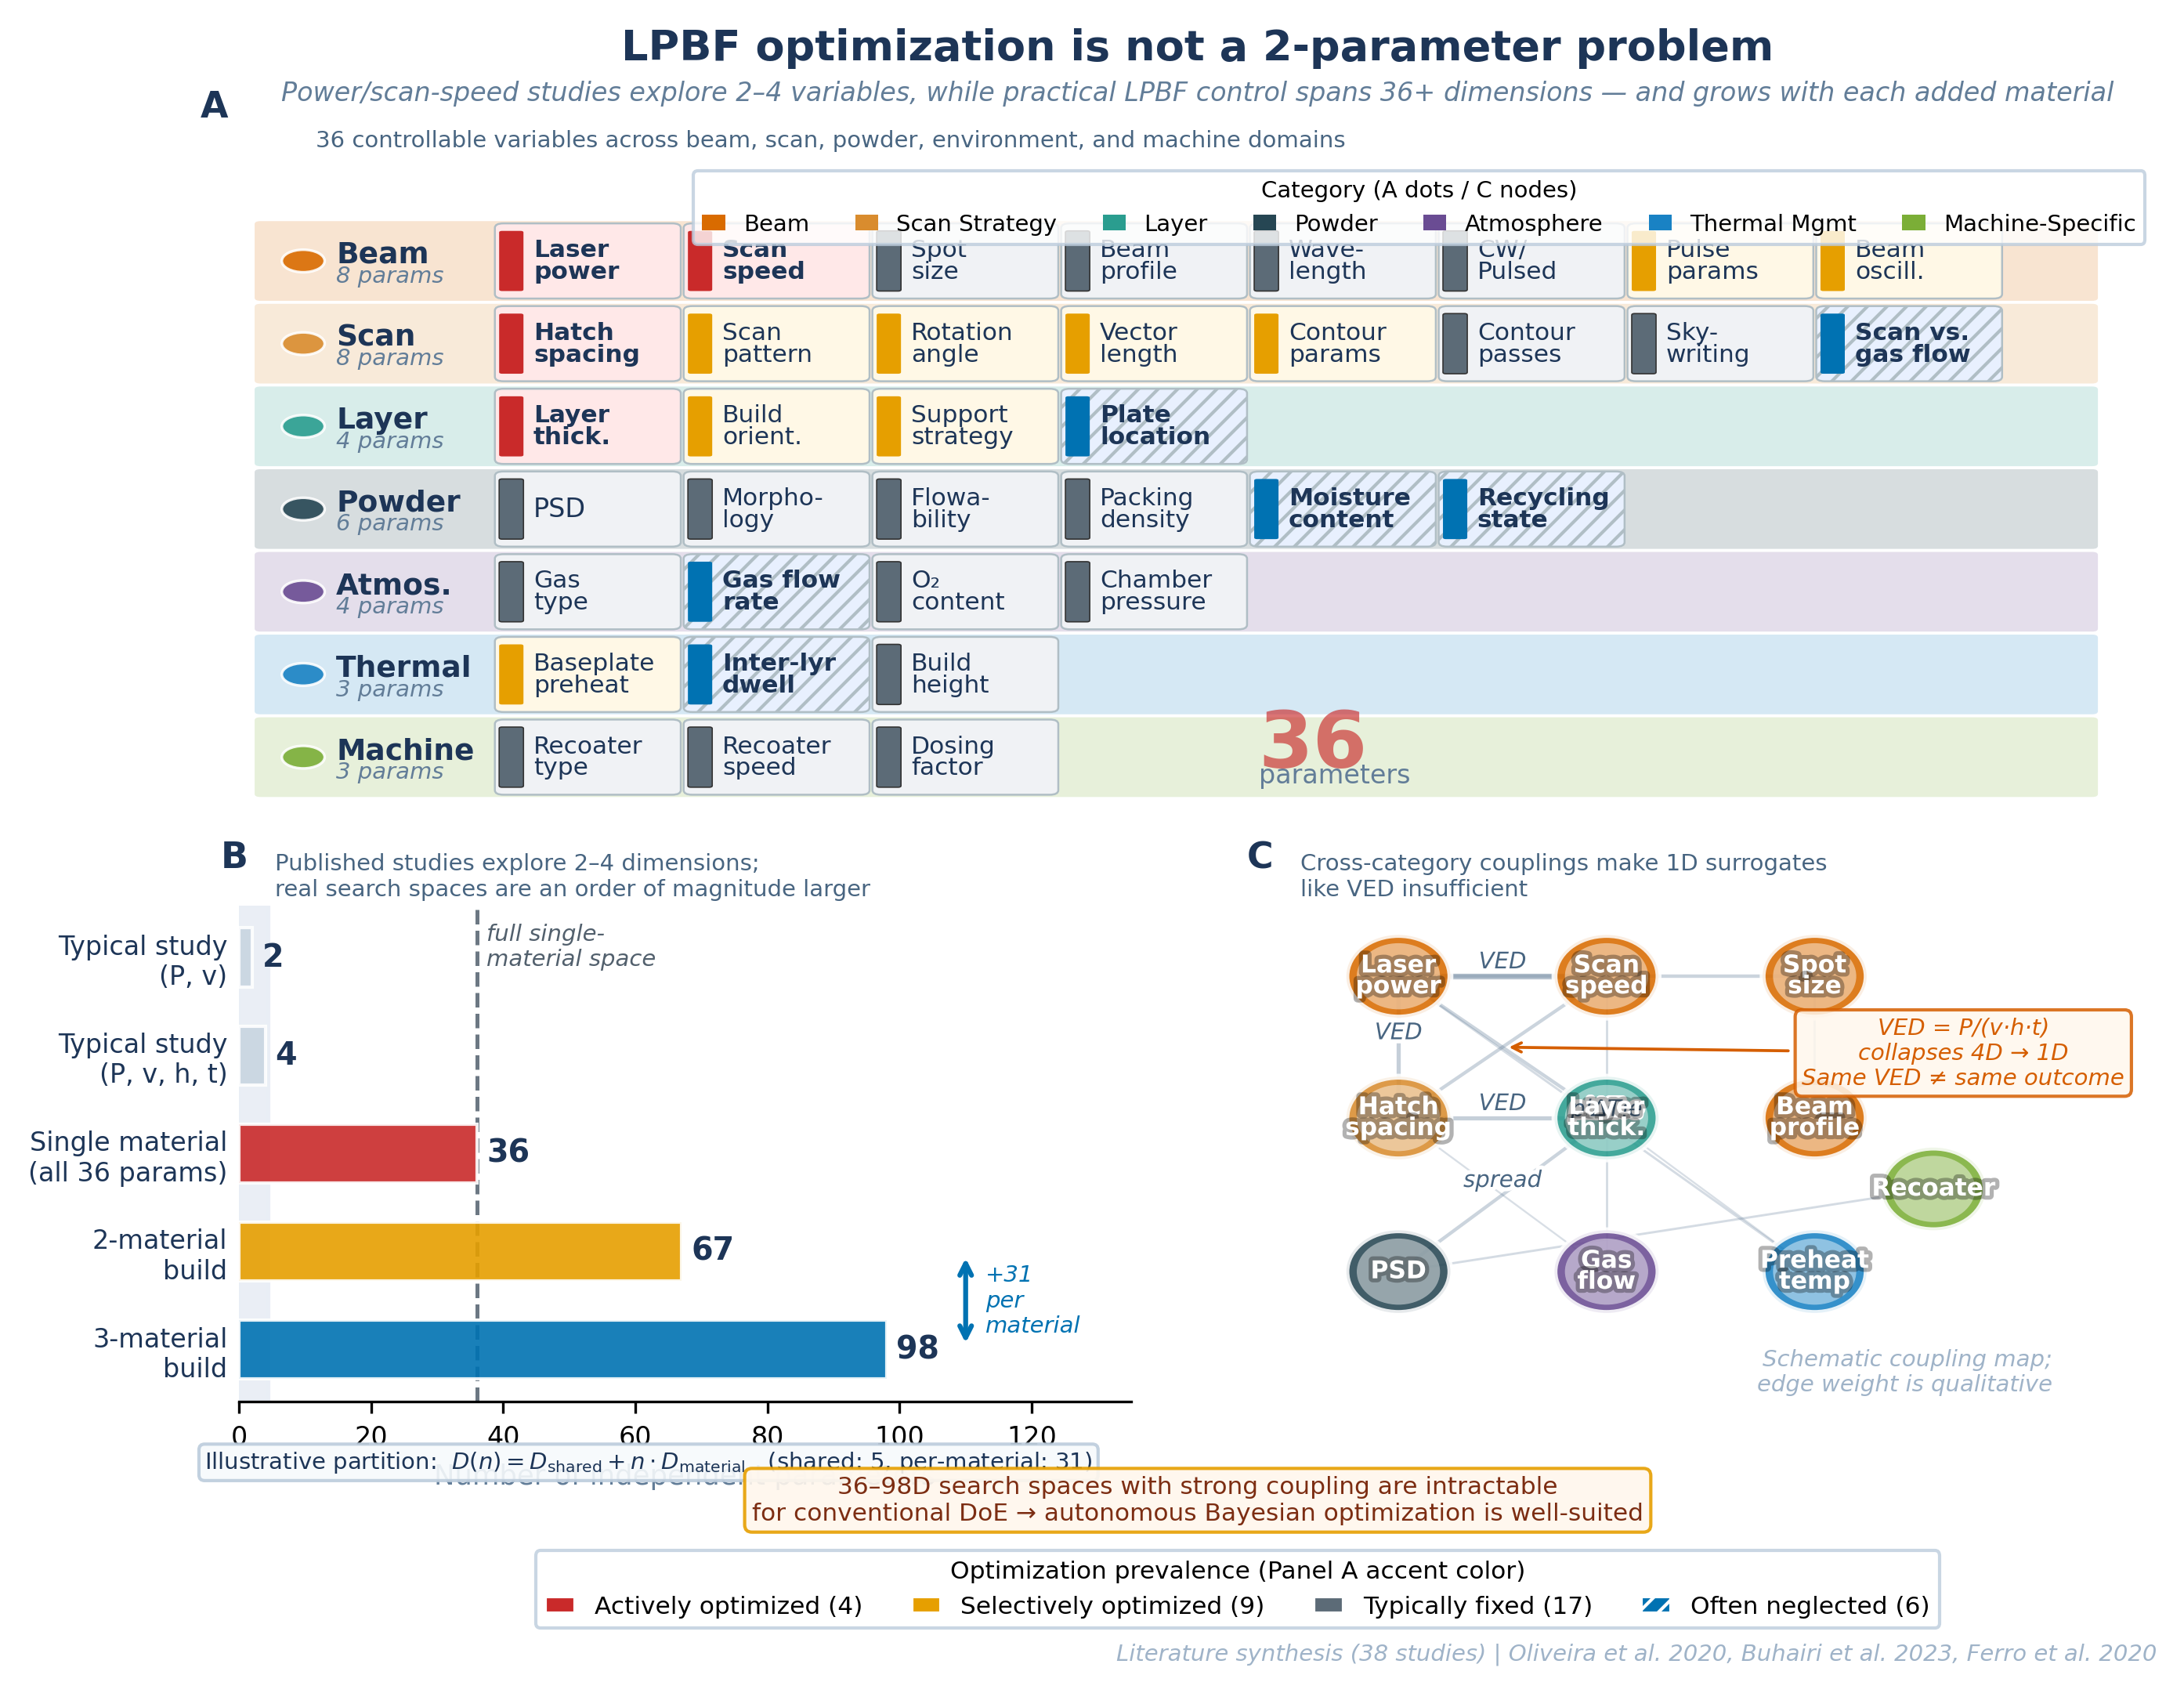
\includegraphics[width=0.85\textwidth]{../figures/lpbf_parameter_space.png}
  \caption{LPBF parameter space taxonomy. Tile grid showing the 36 key process parameters organized by category (laser, powder, geometry, atmosphere, post-processing), illustrating the high-dimensional optimization space addressed by FLAIME's BOFN framework.}
  \label{fig:lpbf-params}
\end{figure}

\begin{figure}[ht]
  \centering
  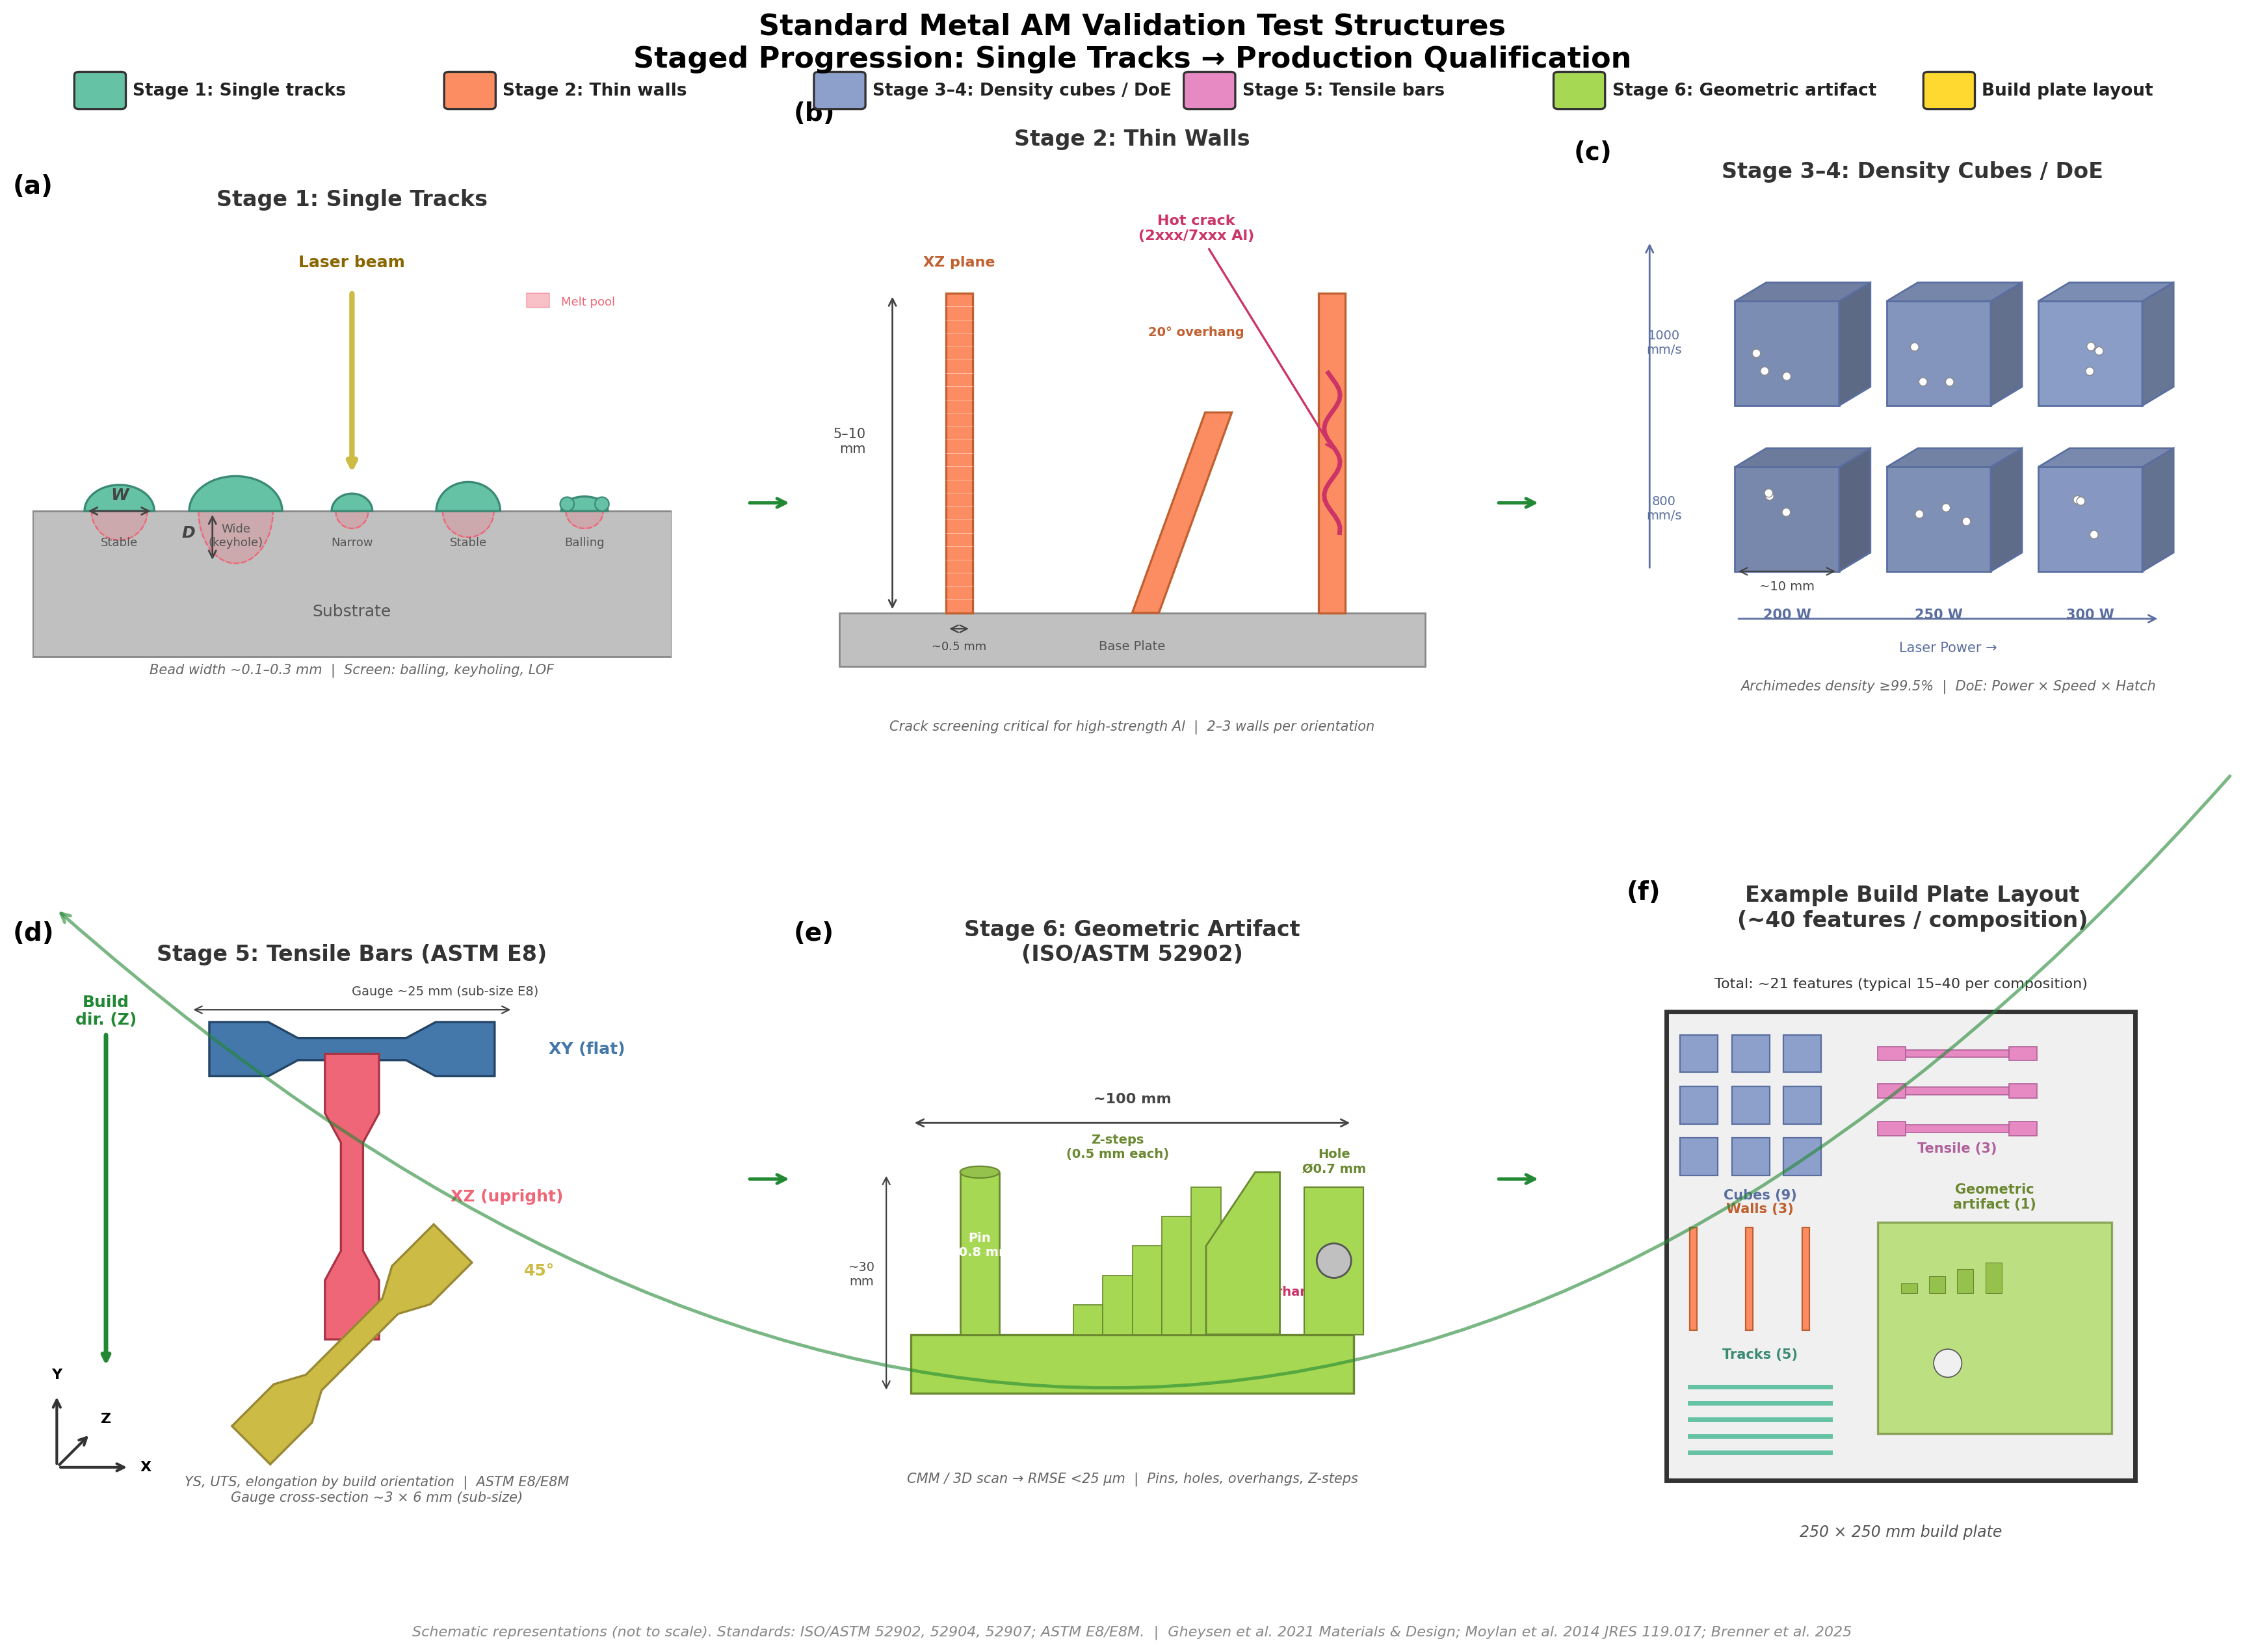
\includegraphics[width=0.85\textwidth]{../edison-trajectories/fig-am-test-structures-schematics.png}
  \caption{AM test structure progression. Illustrative build-plate-layout schematics (not to scale; the Aconity MIDI plate at UofU is 170\,mm diameter circular, $\sim$22{,}700\,mm$^{2}$ usable area) showing the minimum viable specimen (MVS) hierarchy: single tracks for melt-pool characterization, $5\times5\times5$\,mm density cubes for densification screening ($\geq$99.5\% relative density gate), and ASTM~E8 sub-size tensile bars for mechanical property evaluation.}
  \label{fig:am-test-structures}
\end{figure}

\begin{figure}[ht]
  \centering
  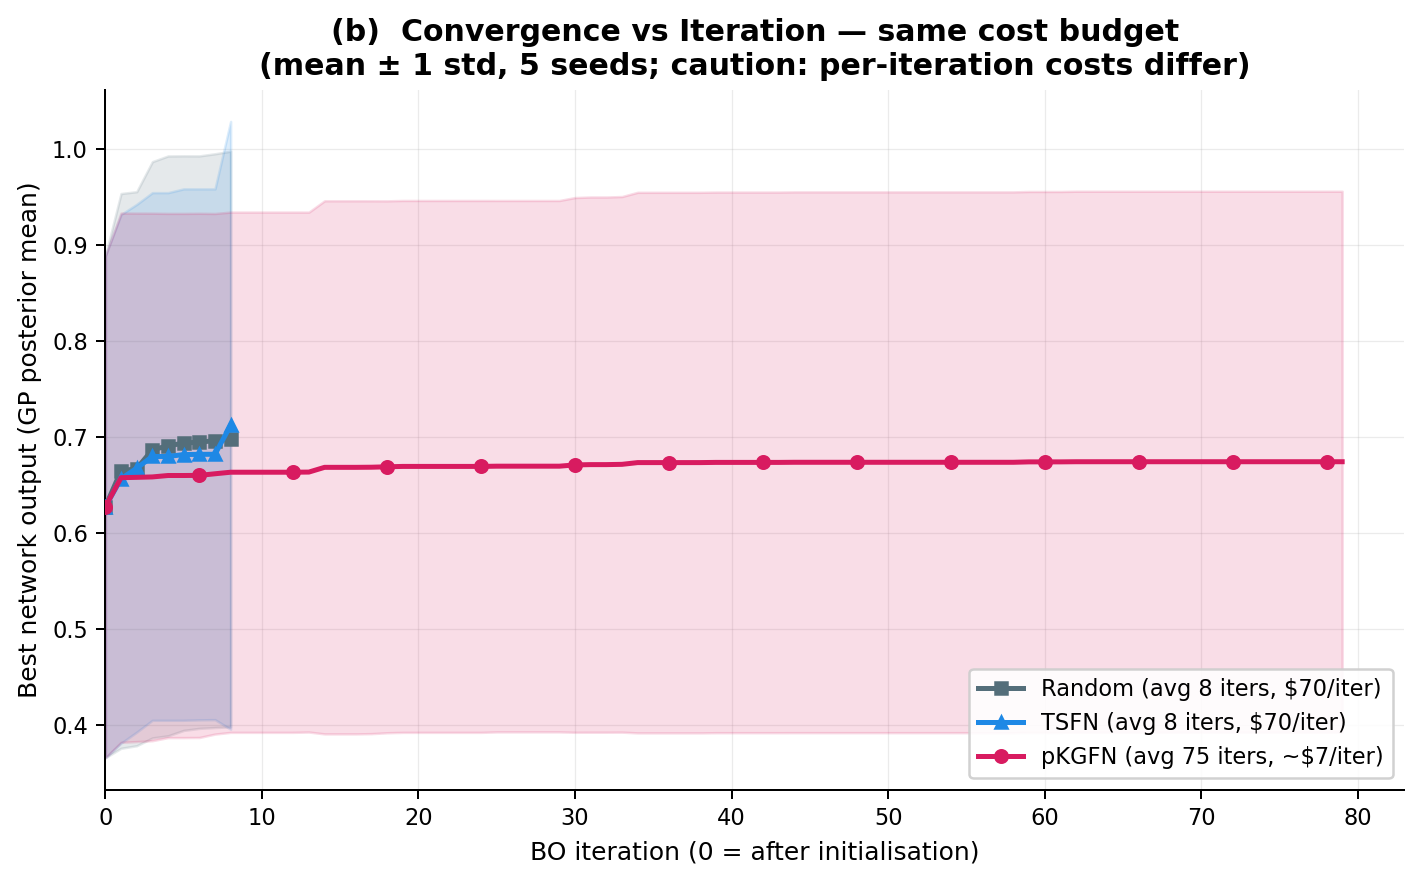
\includegraphics[width=0.85\textwidth]{../benchmarks/figures/pkgfn_convergence.png}
  \caption{Supplementary pKGFN benchmark: convergence vs.\ BO iteration under the same \$1,190 budget. pKGFN completes $\sim$75 partial-evaluation iterations ($\sim$\$7/iter) in the budget where TSFN/Random fit only $\sim$8 full-pipeline iterations (\$70/iter), illustrating the iteration density advantage of partial evaluations.}
  \label{fig:pkgfn-supplementary}
\end{figure}

\begin{figure}[!htbp]
  \centering
  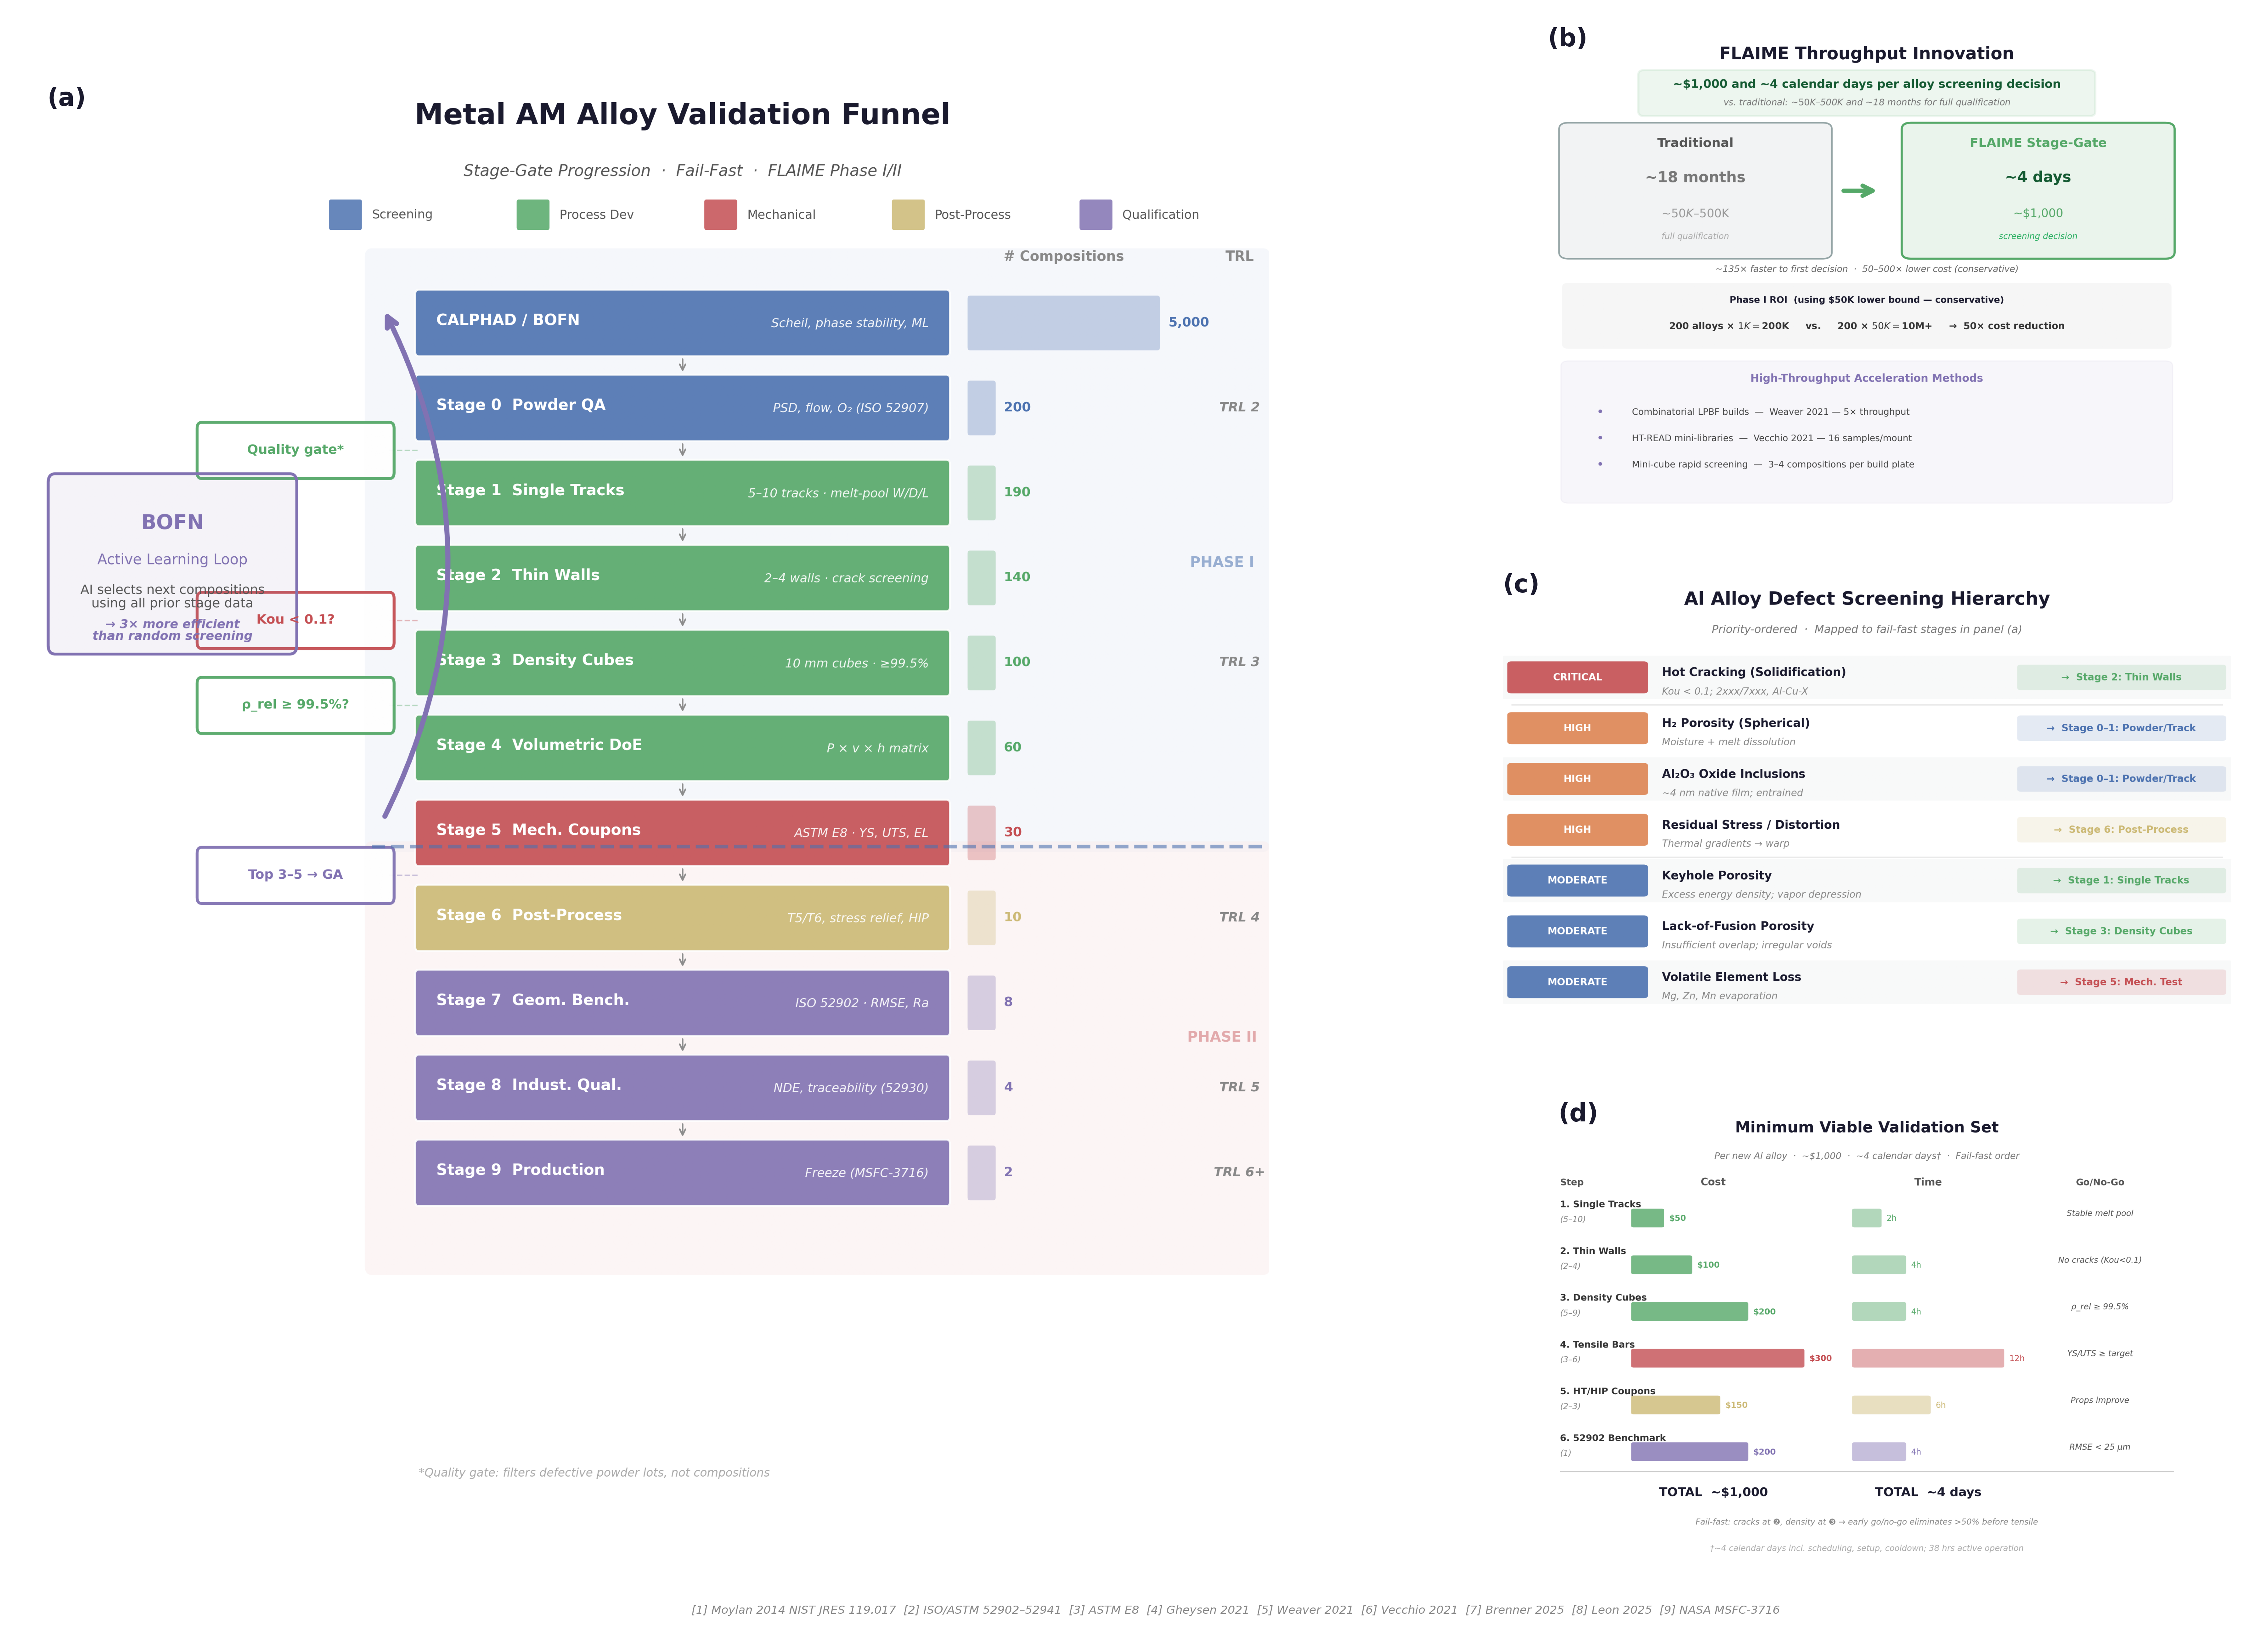
\includegraphics[width=0.85\textwidth]{../figures/composite_4panel.png}
  \caption{FLAIME experimental framework (overview figure relocated from Methods for narrative page-budget compliance): (a)~multi-fidelity stage-gate pipeline with fail-fast screening, (b)~throughput vs.\ traditional alloy development, (c)~Al alloy defect screening hierarchy, (d)~minimum viable validation set per alloy.}
  \label{fig:composite}
\end{figure}

\bigskip\noindent\rule{\textwidth}{0.4pt}
\fi
%%% END UNUSED-FULL-DETAIL

\textbf{BYU Materials Discovery Laboratory (Lead Institution).}
The PI's dedicated laboratory space in the Department of Mechanical Engineering
houses an \textbf{AMAZEMET rePOWDER ultrasonic atomizer with induction
crucible module} (scheduled delivery April~30, 2026; week-long
vendor-led commissioning and training scheduled).  The rePOWDER accepts
mixtures of elemental powders packed into machined high-purity aluminum
crucibles (serving as both vial replacement and compaction chamber with
press-fit lid), enabling high compositional design freedom; the
\textbf{BYU Prototyping Lab} machines these crucibles in-house.  The
powder metallurgy lab is equipped for powder metallurgy and LPBF
workflows---industrial dehumidification, fume hood, electrical, inert-gas,
compressed-air, and chilled-water service installed in coordination with
EH\&S, sized for both the AMAZEMET rePOWDER induction-atomization workflow
and the co-located LPBF workflow.  Powder characterization
is performed on-site via the \textbf{BYU Microscopy Center}
(\url{https://microscopy.byu.edu}; SEM/EDS, EBSD, FIB); tensile and
mechanical testing are directly adjacent (Instron 100~kip Landmark and
20~kip 809 A/T).  Powder metallurgy and mechanical-testing spaces are
connected by an internal door with no public-corridor traversal, a
layout amenable to subsequent robotic integration for future hardware
expansion.

\textbf{Partner LPBF Access.}
Laser powder bed fusion is provided through \textbf{Prof.\ Ashley Spear's
laboratory at the University of Utah} (Aconity~MIDI; 170\,mm $\varnothing$
build plate, open-parameter architecture, 200--1000\,W fiber laser), ideal
for rapid alloy screening; access and preliminary AlSi10Mg baseline prints
are confirmed by letter (Appendix~7).

\textbf{Computing Resources.}
BYU's \textbf{Office of Research Computing} operates a SLURM-managed HPC
cluster ($\sim$28{,}000 CPU cores, 367~GPUs incl.\ NVIDIA H200/H100/A100/L40S,
$>$180\,TB memory across 616 nodes; \url{https://rc.byu.edu}) allocated via
fairshare at no direct project cost, supporting parallel TC-Python CALPHAD
sweeps and BoTorch/GPyTorch surrogate training.  If awarded, we will
additionally request a \textbf{DOE HPC allocation} (e.g., NERSC or OLCF) to
scale campaign-scale Bayesian optimization and AM-process simulations.

\textbf{Partner Facilities (letters in Appendix~7).}
\textbf{Valimet} (Stockton, CA; gas-atomization scale-up of down-selected
compositions, BYU subrecipient with $\geq$20\% Valimet entity cost share);
\textbf{Thermo-Calc Software/AB} (TCAl10, TCMG6, AM~Module licenses and
calibration collaboration; commercial vendor providing software and
technical-staff support via BYU procurement);
\textbf{AMAZEMET} (rePOWDER commissioning, operator training, and technical
support; commercial vendor procured by BYU).

\textbf{Safety \& Powder Handling.}
Benchtop fume hoods, half-mask respirators with certified training, and a
Nilfisk ATEX-rated metal-powder vacuum support safe handling; protocols
were developed with BYU EH\&S.

\bigskip\noindent\rule{\textwidth}{0.4pt}

% ============================================================================
%  APPENDIX 3: EQUIPMENT
%  (0.5 page max; does NOT count against narrative limit)
% ============================================================================
\section*{Appendix 3: Equipment}
\label{app:equipment}

\required{FOA \S IV.C: ``List major items of equipment planned for use
in this project and, if appropriate, identify location and pertinent
capabilities.''  Maximum one page per institution.}

\noindent
Major equipment by workflow (institution in parentheses):
\begin{itemize}\setlength{\itemsep}{0pt}\setlength{\parskip}{0pt}\setlength{\topsep}{2pt}\setlength{\leftmargin}{1em}
  \item \textit{Powder production:} \textbf{AMAZEMET rePOWDER} ultrasonic atomizer w/ induction-crucible module (BYU; delivery Apr~30, 2026; AMAZEMET engaged as commercial vendor / BYU procurement for commissioning + training); \textbf{Valimet} gas-atomization line (Valimet, Stockton CA; funded BYU subrecipient, scale-up).
  \item \textit{LPBF/AM:} \textbf{Aconity MIDI} (UofU, Prof.\ Spear) --- 170\,mm $\varnothing$ plate, open-parameter, 200--1000\,W fiber laser.
  \item \textit{Characterization:} \textbf{BYU Microscopy Center}
        (SEM/EDS, EBSD, FIB, STEM; Verios~G4, Helios NanoLab~600,
        Apreo~C, Tecnai~F20) --- EDAX TEAM workflow already exercised
        on \flaime{} feedstocks (Si-100, Si-40, AlSi10Mg);
        \textbf{BYU XRD Facility} (Chemistry); \textbf{Agilent 8900
        ICP-MS/MS} (BYU).
  \item \textit{Mechanical testing:} \textbf{Instron 100~kip Landmark} and \textbf{20~kip 809 A/T} servo-hydraulic testers (BYU).
  \item \textit{Heat treatment:} \textbf{Recco} and \textbf{Lucifer} box furnaces (BYU).
  \item \textit{Computing:} \textbf{BYU HPC} ($\sim$28K cores, 367~GPUs incl.\ H200/H100/A100/L40S; SLURM fairshare).
\end{itemize}

%%% BEGIN UNUSED-FULL-DETAIL -- preserved for future reference; not compiled
\iffalse
\smallskip\noindent
Major equipment is grouped by general workflow categories.

% ---------- POWDER PRODUCTION ----------
\medskip\noindent\textbf{\textsc{Powder Production}}

\noindent
\begin{minipage}[t]{0.62\textwidth}\raggedright
\textbf{AMAZEMET rePOWDER Ultrasonic Atomizer with Induction Crucible
Module} (BYU; delivery April~30, 2026).  Custom Al alloy powder production
from elemental powder mixtures packed into machined high-purity Al
crucibles; enables up to 3 compositions/day (M--F) and 1 on Saturday.\\[3pt]
\textbf{Aconity MIDI LPBF System} (UofU, Prof.\ Spear).
170\,mm \textsf{\O} build plate, open-parameter architecture,
200--1000\,W fiber laser; ideal for rapid alloy screening.  The
open-parameter framework maps directly to Thermo-Calc AM~Module
tunable parameters.
\end{minipage}\hfill
\begin{minipage}[t]{0.17\textwidth}
\centering
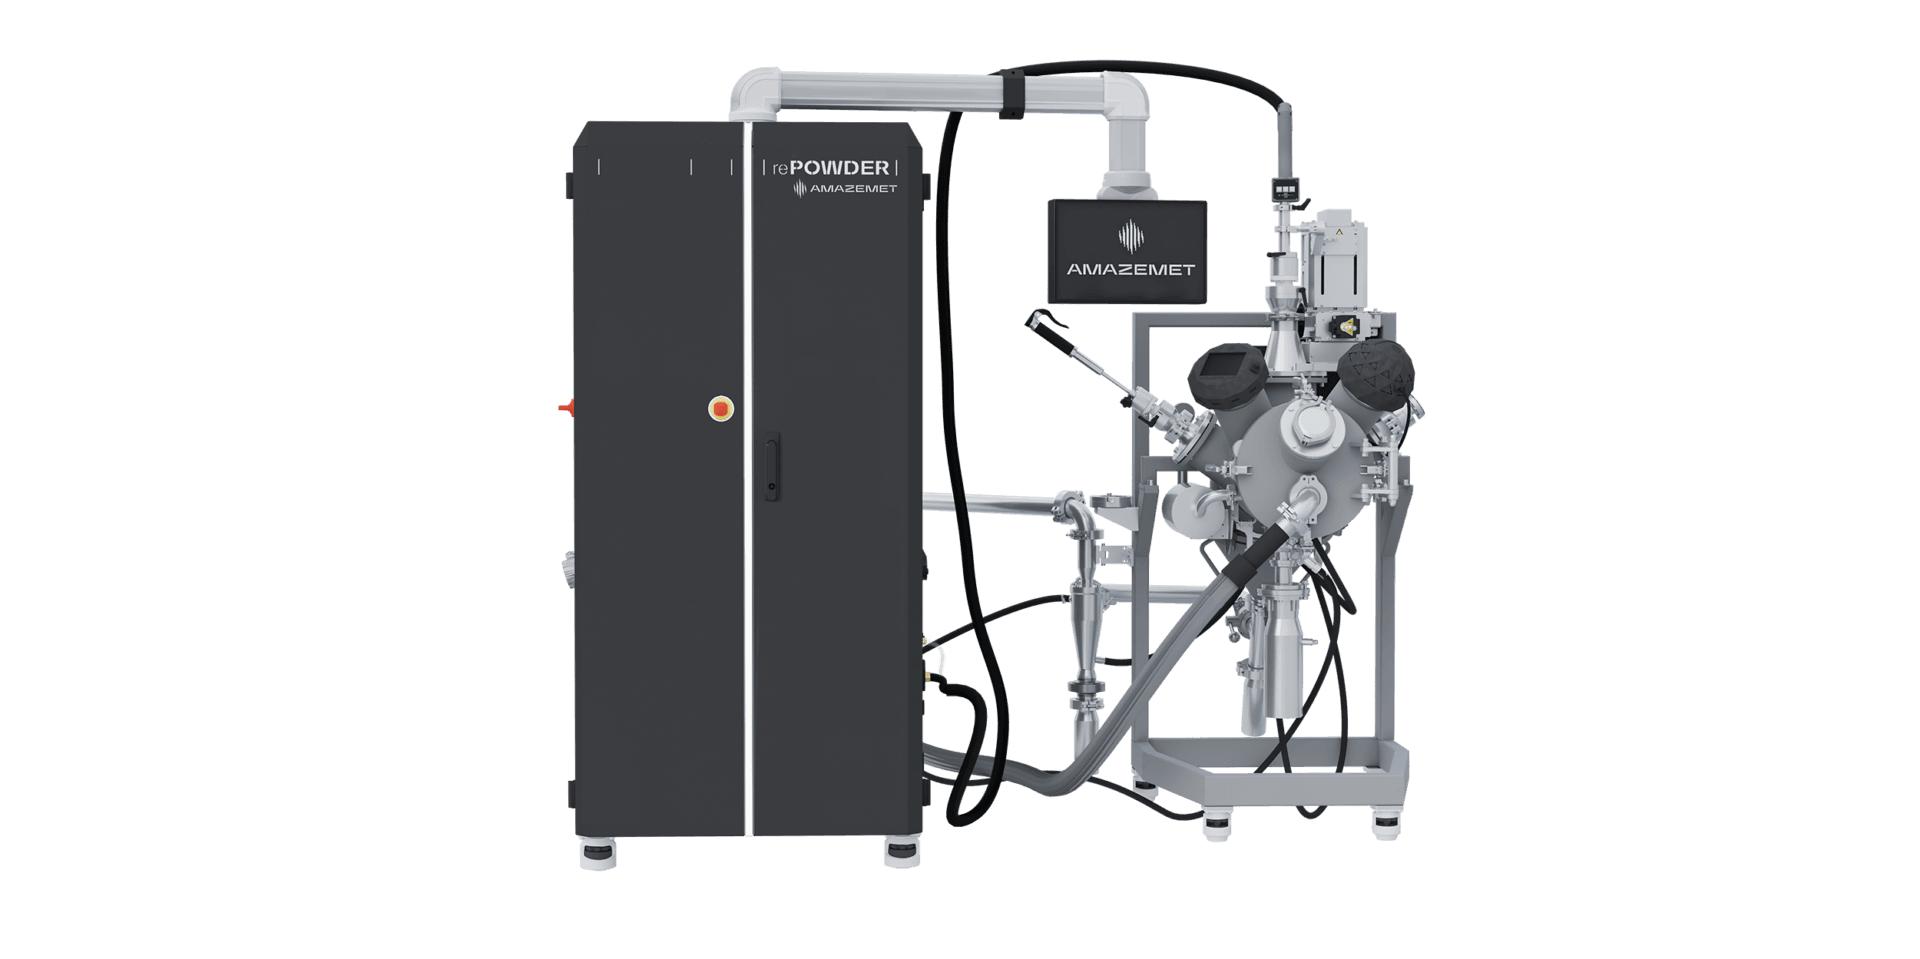
\includegraphics[width=\linewidth]{amazemet-repowder}\\[-2pt]
{\tiny AMAZEMET rePOWDER}
\end{minipage}\hfill
\begin{minipage}[t]{0.17\textwidth}
\centering
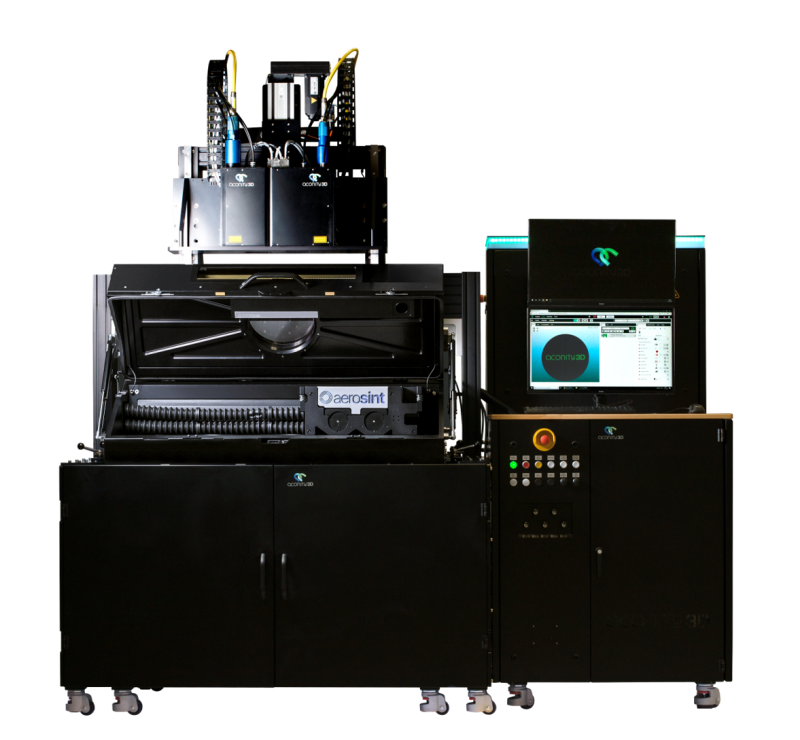
\includegraphics[width=\linewidth]{aconity-midi}\\[-2pt]
{\tiny Aconity MIDI}
\end{minipage}

% ---------- CHARACTERIZATION ----------
\medskip\noindent\textbf{\textsc{Characterization \& Microscopy}}

\noindent
\textbf{BYU Microscopy Center SEM/TEM Suite
(\url{https://microscopy.byu.edu}).}
Four shared-facility electron microscopes; all SEMs accept samples up
to 6~inch diameter with up to 12~inch total length (no stage travel).
Detector/mode matrix:

\begin{center}\small
\begin{tabular}{@{}lcccc@{}}
\toprule
Detector / Mode & Tecnai F20 TEM & Verios G4 UC SEM & Helios NanoLab~600 & Apreo~C SEM \\
\midrule
Everhart--Thornley (ETD, SE/BSE)         &              & $\checkmark$ & $\checkmark$ & $\checkmark$ \\
Backscatter electron (BSE, $Z$-contrast) &              & $\checkmark$ &              & $\checkmark$ \\
Energy-dispersive X-ray (EDXA/EDS)       & $\checkmark$ & $\checkmark$ & $\checkmark$ & $\checkmark$ \\
Electron backscatter diffraction (EBSD)  &              &              & $\checkmark$ & $\checkmark$ \\
Cathodoluminescence (CL)                 &              &              &              & $\checkmark$ \\
Focused ion beam (FIB, Ga$^{+}$)         &              &              & $\checkmark$ &              \\
Immersion lens (high-res mode)           &              & $\checkmark$ & $\checkmark$ &              \\
Through-the-lens detector (TLD, SE)      &              & $\checkmark$ & $\checkmark$ &              \\
Optiplan mode (short-WD T1/T2 imaging)   &              &              &              & $\checkmark$ \\
Low-vacuum mode (dry/uncoated samples)   &              &              &              & $\checkmark$ \\
Scanning transmission (STEM)             & $\checkmark$ & $\checkmark$ & $\checkmark$ &              \\
T1 / T2 backscatter + SE detectors       &              &              &              & $\checkmark$ \\
\bottomrule
\end{tabular}
\end{center}

\smallskip
\noindent\textbf{FEI Tecnai G2 F20 TEM/STEM} (Schottky FEG, 20--200\,kV).
TEM point resolution 0.19~nm, line resolution 0.102~nm, magnification
25$\times$--1{,}000{,}000$\times$; STEM HAADF resolution 0.14~nm; energy
spread $\leq$0.7~eV; probe current $>$0.5~nA in a 1~nm spot; eucentric
CompuStage; accessories include HAADF, XEDS (Pathfinder), PEELS, EFTEM
monochromator, low-background double-tilt and heating/cooling holders.
Used for nanoscale precipitate characterization (L1$_2$ Al$_3$(Sc,Zr,Er),
$\theta'$-Al$_2$Cu) and STEM-EDS line scans across solidification
interfaces.

\smallskip
\noindent\textbf{ThermoScientific Verios G4 UC SEM} (Elstar monochromated
XHR FESEM column). Landing energies 20~eV--30~keV with beam deceleration
(stage bias $-50$\,V to $-4$\,kV); 0.6~nm resolution at 15~kV, 0.7~nm at
1~kV; probe current 0.8~pA--100~nA; piezo 5-axis 100$\times$100~mm
stage; in-column/in-lens SE+BSE (TLD-SE, TLD-BSE, ICD, MD), ETD,
retractable STEM~3+ and DBS detectors; UltraDry Premium EDS (60~mm$^2$,
129~eV at Mn K$\alpha$) with Pathfinder XEDS. Primary workhorse for
high-resolution surface morphology of atomized powders and polished
LPBF cross-sections.

\smallskip
\noindent\textbf{FEI Helios NanoLab~600 DualBeam FIB/SEM} (Elstar UHR
immersion lens FESEM 350~V--30~kV; Tomahawk Ga$^{+}$ ion column
0.5--30~kV, 0.1~pA--65~nA, 15 apertures; coincident-point ion-beam
resolution 2.5~nm at 30~kV). TLD-SE/BSE, ETD, EDS, and EBSD detectors;
OmniProbe AutoProbe~200 in-situ lift-out; 5-axis motorized stage
(XY~150\,mm piezo, tilt accuracy 0.1$^{\circ}$). Enables site-specific
TEM/APT lamella preparation from LPBF builds and cross-sectional serial
sectioning of melt-pool boundaries.

\smallskip
\noindent\textbf{ThermoFisher Apreo~C SEM} (low-vac FESEM with T1/T2
in-chamber detectors; Optiplan mode). Routine characterization,
low-vacuum/uncoated fine-powder imaging, and CL + EBSD for grain-level
texture on polished LPBF cross-sections.

\begin{center}
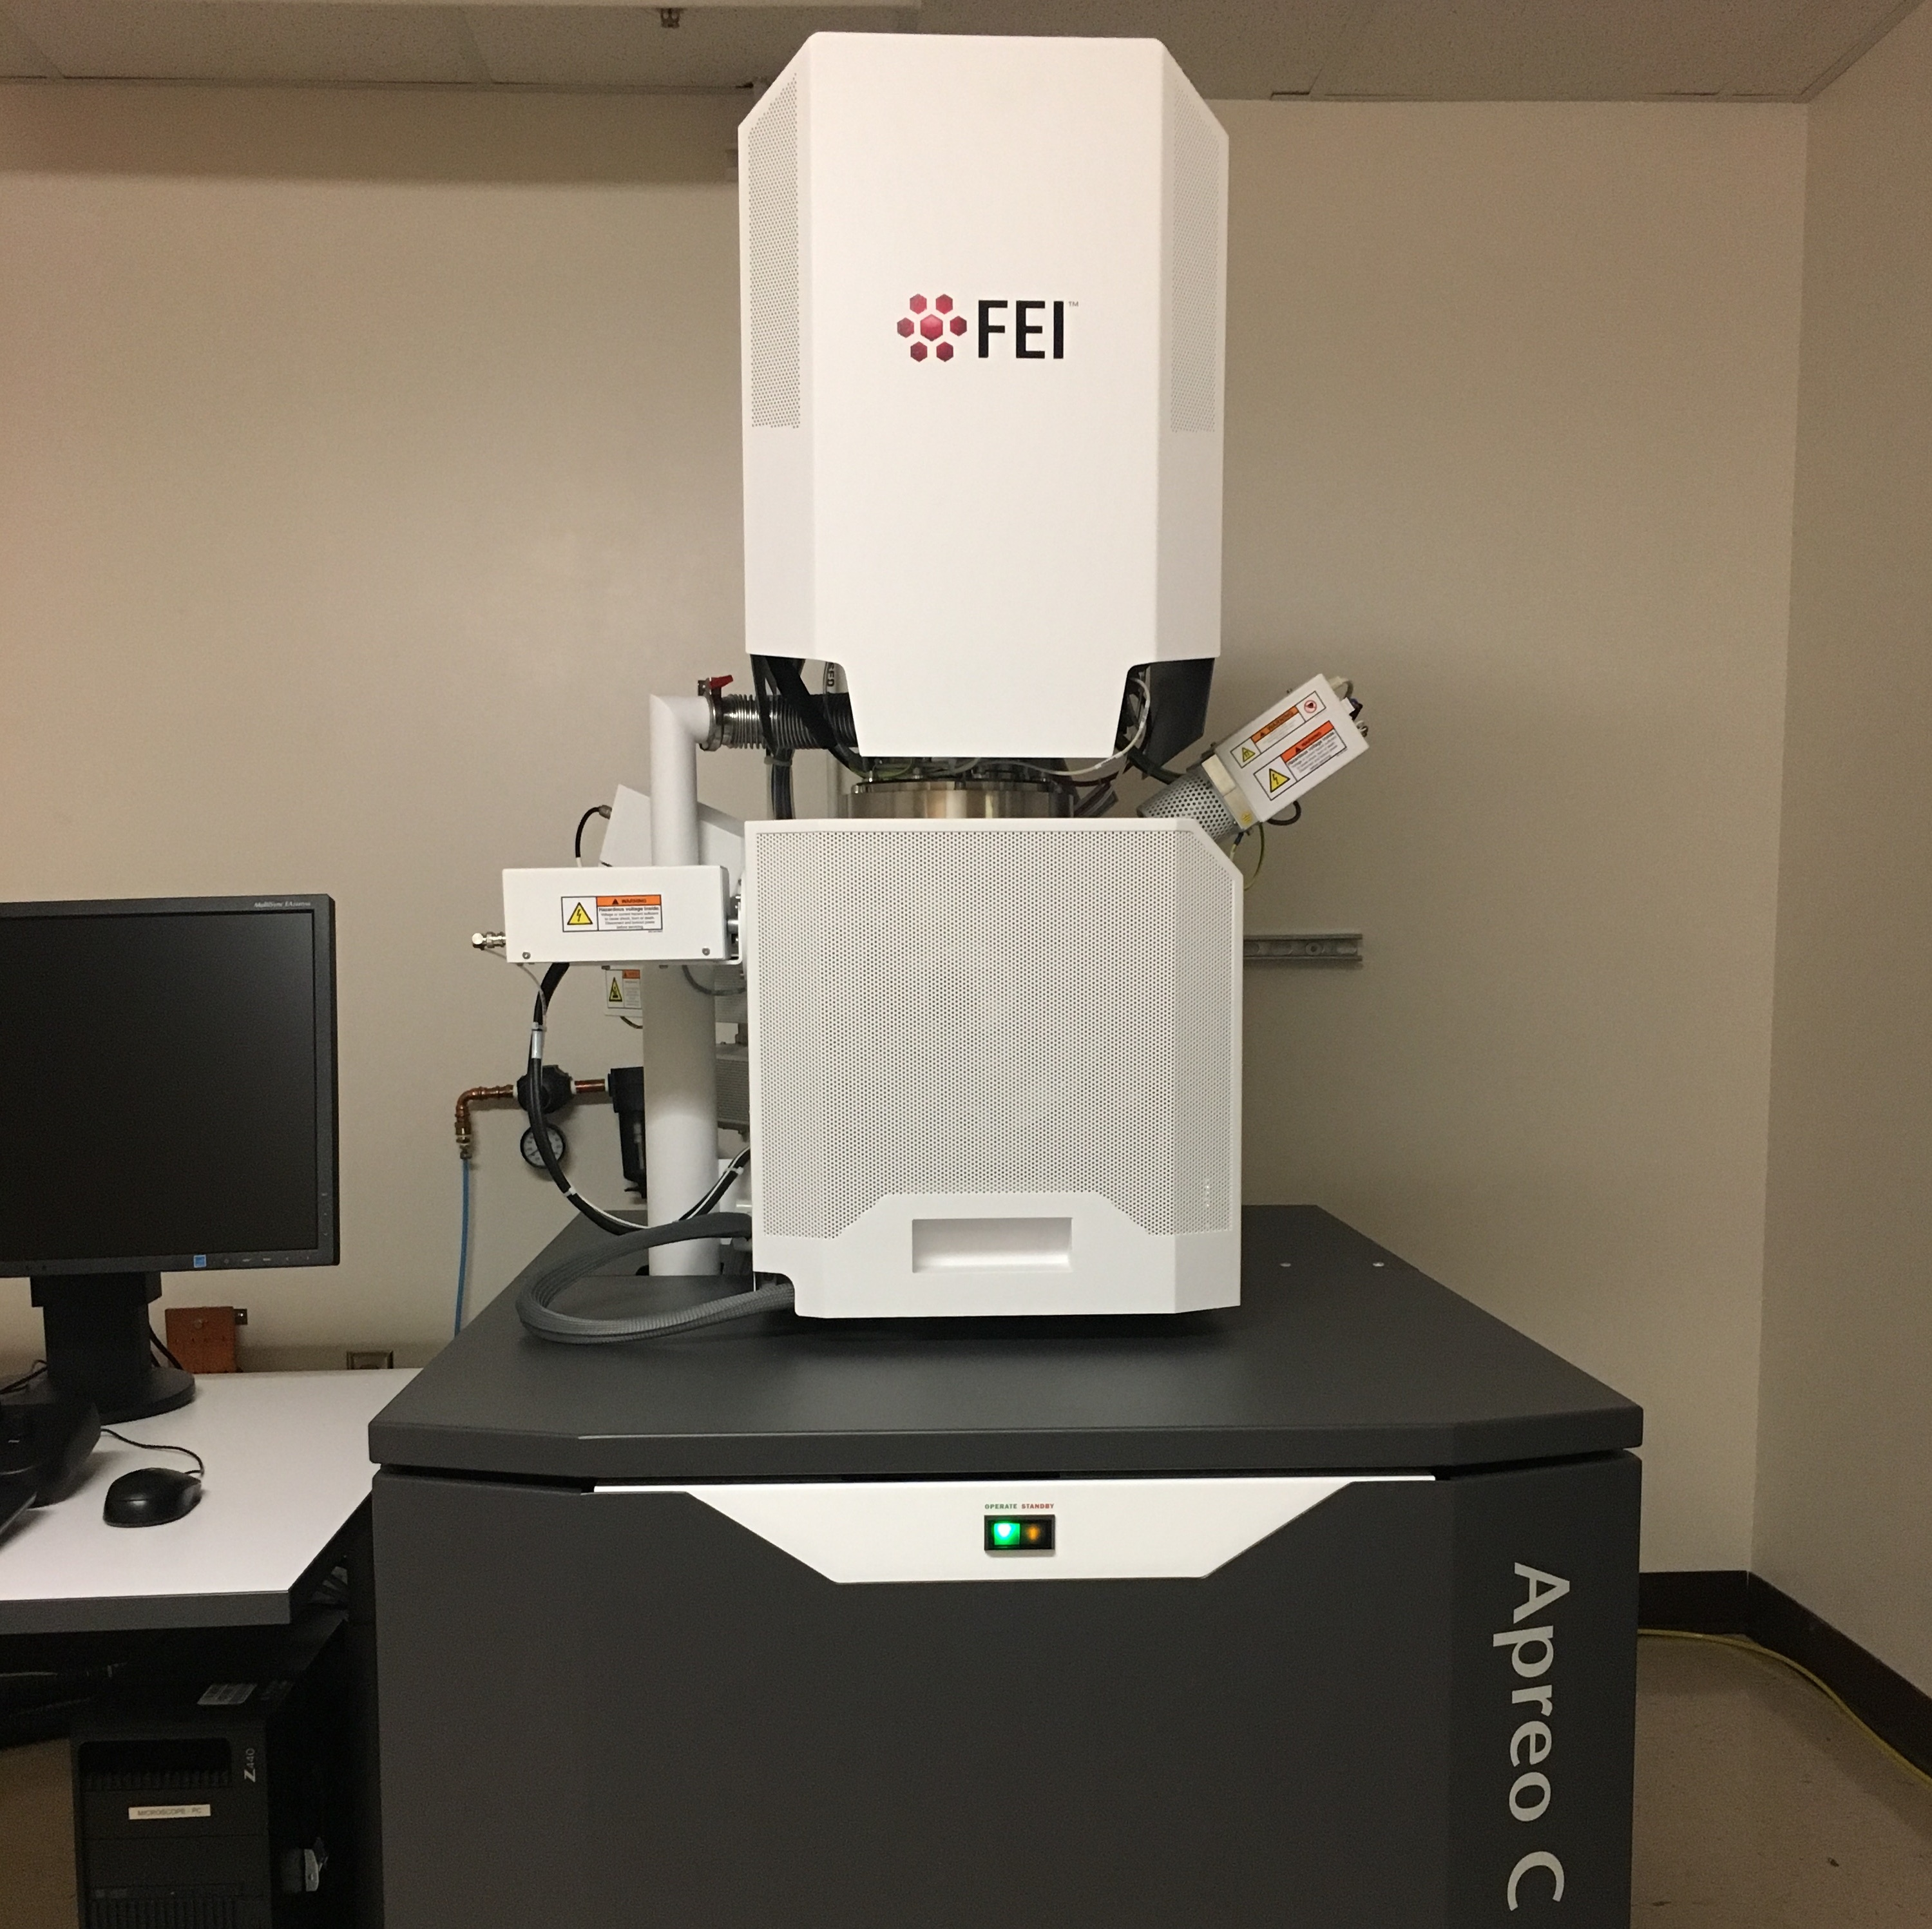
\includegraphics[width=0.22\linewidth]{apreo-sem}\hfill
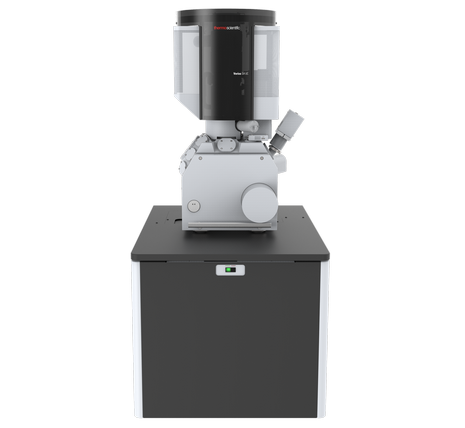
\includegraphics[width=0.22\linewidth]{verios-sem}\hfill
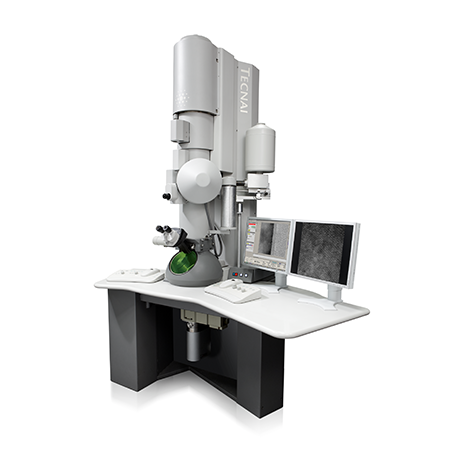
\includegraphics[width=0.22\linewidth]{tecnai-tf20-tem}\hfill
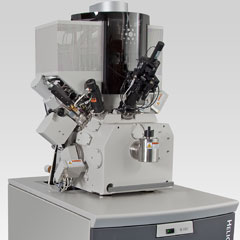
\includegraphics[width=0.22\linewidth]{helios-nanolab}
\\[-2pt]
{\tiny Apreo~C SEM \hfill Verios G4 UC SEM \hfill Tecnai F20 TEM \hfill Helios NanoLab~600}
\end{center}

\smallskip
\noindent
\textbf{Keyence VHX-7000 Optical Microscope} (BYU).
High-resolution digital microscope with automated tiling,
depth-of-field composition, and quantitative measurement;
metallography and defect screening.

\smallskip
\noindent
\textbf{BYU XRD Facility}
(\url{https://labs.chem.byu.edu/xrd-facility}).  Phase identification
and crystallographic analysis.

\smallskip
\noindent
\textbf{Phantom v1610 High Speed Camera} (BYU).
Up to 16{,}000\,fps at full resolution (1280$\times$800);
includes tripod, laptop, software, and lighting.
Also available: FLIR E50 thermal camera,
Chronos 2.1-HD ($\leq$1000\,fps at 1080p),
and Sony high-speed camera (for powder-flow and melt-pool visualization).

\smallskip
\noindent
\textbf{Hommel Profilometer Roughness Tester} (BYU).
Surface-roughness measurement with 0.01\,\textmu{}m precision;
$R_a$ roughness value calculation for LPBF surface quality assessment.

\smallskip
\noindent
\textbf{BYU Geology Dept.\ Analytical Labs}
(\url{https://geology.byu.edu/labs}).  XRF, ICP-OES, and powder XRD
available for cross-validation of elemental composition and
phase identification.

\smallskip
\noindent
\textbf{BYU Spectroscopic Facility:} XPS surface analysis
(\url{https://labs.chem.byu.edu/byu-spectroscopic-facility/surface-analysis});
\textbf{Agilent 8900 ICP-MS/MS}
(\url{https://labs.chem.byu.edu/byu-spectroscopic-facility/atomic-analysis})
for authoritative elemental composition verification.

\medskip
\noindent\textbf{Quantitative Compositional Analysis Methodology.}
The FLAIME \elementcount-element Al-alloy palette (Al + \elementlisttex{}) spans every regime that stresses a
single-technique compositional workflow: light elements at or below the
SDD window (Li~K$\alpha$ at 54~eV is effectively inaccessible to EDS and
must be quantified spectrochemically), closely spaced light-element
K-lines (Mg~K$\alpha$ 1.253 / Al~K$\alpha$ 1.486 / Si~K$\alpha$
1.740~keV, ${\sim}230$~eV apart against the ${\sim}120$--$135$~eV
silicon-drift-detector (SDD) full-width-at-half-maximum (FWHM) at
Mn~K$\alpha$), transition-metal K-line neighbours (Sc/Ti ${\sim}420$~eV,
Cr/Mn/Fe spaced by ${\sim}500$~eV with K$\beta$/K$\alpha$ crossover), and
rare-earth/heavy L-line overlaps with transition-metal K-lines
(Ce~L$\alpha$~4.84 vs Ti~K$\beta$~4.93 / V~K$\alpha$~4.95; Er~L$\alpha$~6.95
vs Fe~K$\beta$~7.06; Zr~L$\alpha$~2.04 requires L-line quant unless
accelerating voltage is raised to excite Zr~K$\alpha$ at 15.78~keV).
Trace-level grain-refiner and strengthener loadings ($<0.5$~wt\% Sc, Zr,
Er, Ce) routinely push against EDS detection limits (${\sim}0.1$~wt\%
under optimized conditions), and reactive solutes (Mg, Li, rare earths)
preferentially segregate to powder surfaces and evolve with reuse. No
single instrument resolves all of these simultaneously; FLAIME therefore
adopts a cross-validated multi-technique hierarchy, with the Mg/Al-Si-Mg
case serving as the canonical worked example because the peak overlap,
trace threshold, and surface-segregation behaviour there are simply the
most-studied instance of issues that recur across the palette:
\begin{itemize}[leftmargin=*,nosep]
  \item \textbf{Rapid screening (semi-quantitative).} Carbon-tape-mounted
        loose-powder SEM-EDS for phase ID, homogeneity checks, and
        particle-by-particle triage~\cite{groarke_2021_b9780128}; treated as
        qualitative only---curved powder surfaces violate the flat-specimen
        assumption of ZAF (atomic-number / absorption / fluorescence) and
        $\varphi(\rho z)$ (depth-distribution) matrix corrections.
  \item \textbf{Standards-based quantitative SEM-EDS.} Epoxy-mounted cross-
        sections polished to a 0.05~\textmu{}m colloidal-silica mirror finish
        with ${\sim}10$~nm conductive carbon coat, per ASTM~E1508 (quantitative
        EDS) and ASTM~E1078 (mounting).  K-ratios against pure-element and
        stoichiometric-compound standards matched to each composition's
        active element set (e.g., Al / Si / MgO / Al$_2$O$_3$ for Al-Si-Mg;
        Mn / Cr / Fe metal foils for transition-metal-rich systems; CeO$_2$
        / Er$_2$O$_3$ / Sc$_2$O$_3$ / ZrO$_2$ for RE-containing and
        grain-refined alloys) with $\varphi(\rho z)$ matrix corrections.
        Accelerating voltage is tuned per alloy family---15--20~kV as the
        default, raised toward 25--30~kV when Zr~K$\alpha$ or Sn~K$\alpha$
        access is needed, lowered toward 10--12~kV to preserve light-element
        ($Z{\leq}14$) sensitivity.  Dead time $\leq 10\%$, $N=5$--$10$
        spectra per target, targeting particle \emph{interiors} away from
        the oxide-affected outer ring.  This route reaches ${\sim}1$--$2\%$
        relative error on major elements in controlled studies versus the
        ${\sim}25$--$30\%$ envelope of his\-tor\-i\-cal standardless
        quantification.
  \item \textbf{High-resolution validation (wavelength-dispersive
        spectroscopy / electron probe microanalysis, WDS/EPMA).} Reserved
        for close peak-overlap families (Mg~K$\alpha$/Al~K$\alpha$, Sc~K$\alpha$/Ti~K$\alpha$
        / Ca~K$\beta$, Ce~L$\alpha$/Ti~K$\beta$/V~K$\alpha$,
        Er~L$\alpha$/Fe~K$\beta$) and for trace species $<0.2$~wt\% where
        EDS is marginal; accessed through the BYU--UofU collaborative
        MRI-in\-stru\-men\-ta\-tion network and used sparingly to anchor
        EDS calibrations.
  \item \textbf{Authoritative bulk verification (ICP-MS/ICP-OES).} BYU
        Agilent~8900 ICP-MS/MS for certified sub-ppm multi-element bulk
        chemistry across the full palette (the only accurate route for Li,
        and the primary reference for trace Sc/Zr/Er/Ce), cross-validated
        against BYU Geology Dept.\ ICP-OES/XRF.  Immune to powder
        topography and surface oxides, this is the ground truth against
        which SEM-EDS is benchmarked: FLAIME's provenance schema audits
        every $k{=}10^{\text{th}}$ composition through ICP-MS regardless
        of the EDS result and flags any $>5\%$ relative disagreement for
        re-run.
  \item \textbf{Surface-chemistry and solute-segregation monitoring (XPS).}
        BYU Spectroscopic Facility XPS for depth-profiled characterization
        of native-oxide growth (the Al$_2$O$_3$ shell, ${\sim}4$~nm on
        virgin AlSi10Mg powder, grows to ${\sim}18$--$38$~nm with aging /
        reuse and serves as the reference case) and for surface enrichment
        of reactive solutes---Mg ($4$--$8\times$ bulk as MgAl$_2$O$_4$
        spinel), Li, and rare earths (Ce, Er, Sc)---along with Si subsurface
        depletion.  Reused-feedstock lots are XPS-audited per-campaign;
        oxide-thickness or surface-composition drift beyond a pre-registered
        threshold triggers re-atomization rather than continued reuse.
\end{itemize}
\noindent Every composition is traceable through design target $\to$
Thermo-Calc phase assemblage $\to$ atomized-powder bulk chemistry (ICP-MS)
$\to$ particle-interior EDS on polished cross-sections $\to$ surface-oxide
state (XPS), with instrument, operator, accelerating voltage, standards,
correction model, and prep method tagged in the digital-thread provenance
schema to enable downstream reproducibility and open-data release.

\medskip
% ---------- SAMPLE PREPARATION ----------
\medskip\noindent\textbf{\textsc{Sample Preparation}}

\noindent
\begin{minipage}[t]{0.62\textwidth}\raggedright
\textbf{Metallographic Polishing Lab} (BYU).
PX500 Automatic Polisher (1.5\textquotedbl{} sample pucks),
two PX300 Manual Polishers, non-crystallizing silica vibratory polishers,
fume hood for chemical etching, and electrochemical polisher (Lead PI
has extensive experience with all).  Metallographic polishing and
optical microscopy are both BOFN DAG nodes.\\[3pt]
\textbf{Rolling Mill} (BYU).  Resolution 0.00005\textquotedbl{},
width 6\textquotedbl{}.
\end{minipage}\hfill
\begin{minipage}[t]{0.35\textwidth}
\centering
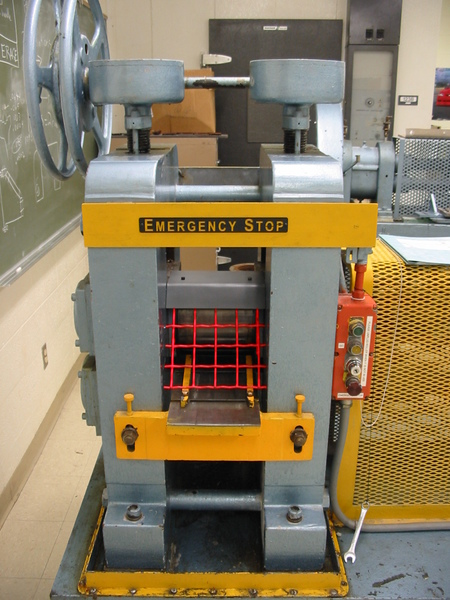
\includegraphics[width=0.9\linewidth]{rolling-mill}\\[-2pt]
{\tiny Rolling Mill}
\end{minipage}

% ---------- MECHANICAL TESTING ----------
\medskip\noindent\textbf{\textsc{Mechanical Testing}}

\noindent
\begin{minipage}[t]{0.62\textwidth}\raggedright
\textbf{100\,kip Landmark Tensile Tester} (BYU).
Tensile/compressive loads; capacity 110{,}000\,lb ($\pm$10\,lb);
stroke 6\textquotedbl{} ($\pm$0.001\textquotedbl{});
specimen width 0--0.83\textquotedbl{},
diameter 0.25--2.02\textquotedbl{}.\\[3pt]
\textbf{20\,kip 809 A/T Tensile Tester} (BYU).
Tensile/compressive/torsional loads; axial capacity 20{,}000\,lb
($\pm$2\,lb); torsional capacity 10{,}000\,in$\cdot$lb.\\[3pt]
\textbf{Impact Tester: Instron Model SI-1D3} (BYU).
Striker weight 66.6\,lb; drop height 4.51\,ft; impact velocity
17\,ft/s; range 0--300\,ft-lbs.  Equipped for Charpy and Izod
impact tests.\\[3pt]
\textbf{Elevated-Temperature Tensile Tester} (BYU). \textit{[TBD specification---placeholder for high-temperature uniaxial tester for Al--Zr L1$_2$ precipitate stability validation at three temperatures; see Activity~2.]}\\[3pt]
\textbf{Vickers Micro Hardness Tester} (BYU).  Surface hardness mapping across samples; used for screening hardness--composition trends before full tensile testing.\\[3pt]
\textbf{Zeiss Xradia Versa 620 Nano-CT} (UofU EMSAL).
Non-destructive 3D defect analysis; in-situ tensile stage
(5\,kN), heating/cooling capability, lab-DCT.
\end{minipage}\hfill
\begin{minipage}[t]{0.17\textwidth}
\centering
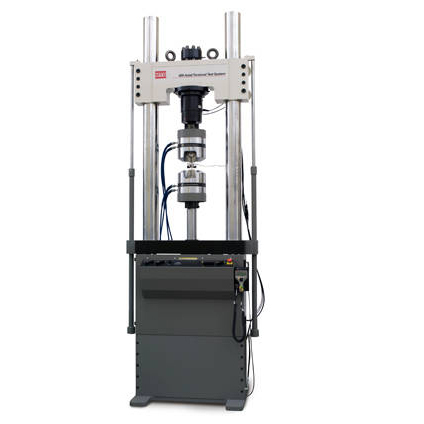
\includegraphics[width=\linewidth]{tensile-100kip}\\[-2pt]
{\tiny 100\,kip Landmark}
\end{minipage}\hfill
\begin{minipage}[t]{0.17\textwidth}
\centering
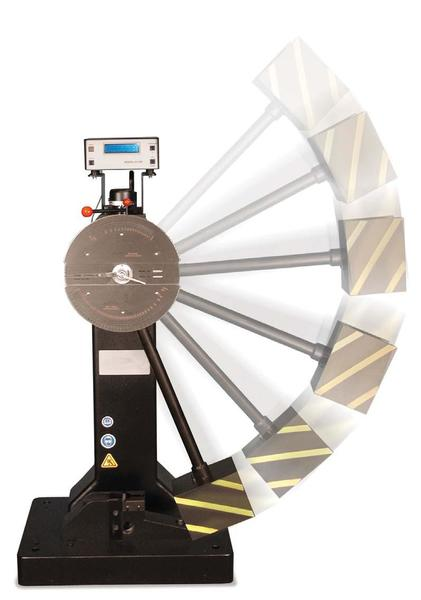
\includegraphics[width=\linewidth]{impact-tester}\\[-2pt]
{\tiny Instron SI-1D3}
\end{minipage}

% ---------- HEAT TREATMENT ----------
\medskip\noindent\textbf{\textsc{Heat Treatment}}

\noindent
\begin{minipage}[t]{0.62\textwidth}\raggedright
\textbf{Recco Furnace} (BYU).
Capacity 12\textquotedbl{}W $\times$ 7\textquotedbl{}H $\times$
19\textquotedbl{}D; max temperature 2250\textdegree{}F;
Ar/N$_2$ atmosphere capability.\\[3pt]
\textbf{Lucifer Furnace} (BYU, CB~121).
Capacity 10\textquotedbl{}W $\times$ 8\textquotedbl{}H $\times$
18\textquotedbl{}D; max temperature 2350\textdegree{}F.\\[3pt]
\textbf{MTI Vacuum Furnace} (BYU).
Capacity 40\,mm diameter $\times$ 200\,mm length; max temperature
1100\textdegree{}C (1000\textdegree{}C continuous); vacuum level
$5.0\times10^{-3}$\,mbar.\\[3pt]
\textbf{CM Hydrogen Furnace} (BYU).
Capacity 3\textquotedbl{} diameter; max temperature 1600\textdegree{}C;
hydrogen, nitrogen, ethylene, and air atmospheres.\\[3pt]
\textbf{Custom Ultra-High-Purity Induction Tube Furnace} (built by Lead PI).
Semi-automated with PID temperature ramping (including rapid ramp/cool);
high-vacuum (turbomolecular pump) or backfilled inert gas;
non-contact 2-color pyrometer through replaceable quartz windows;
custom crucibles/susceptors with sapphire windows.
Max temperature 2500\textdegree{}C.
\end{minipage}\hfill
\begin{minipage}[t]{0.35\textwidth}
\centering
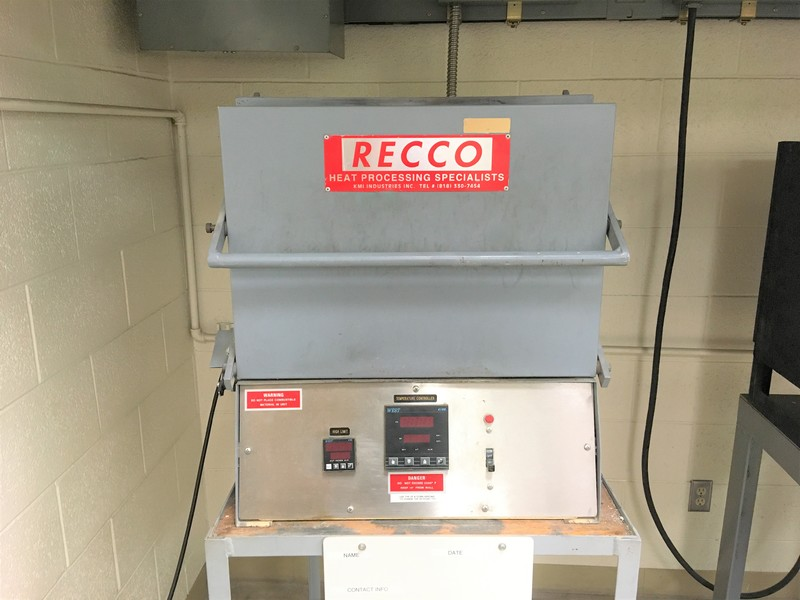
\includegraphics[width=0.45\linewidth]{recco-furnace}%
\hfill
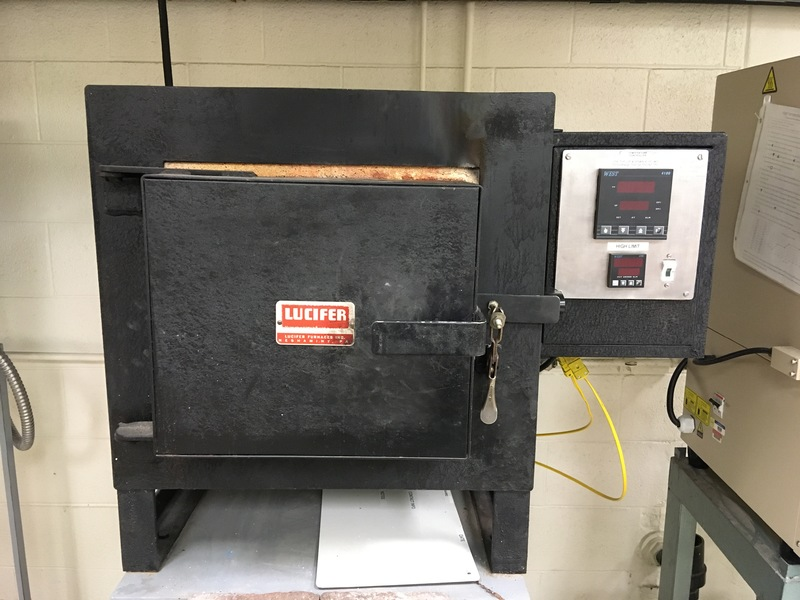
\includegraphics[width=0.45\linewidth]{lucifer-furnace}\\[-2pt]
{\tiny Recco \hfill Lucifer}\\[3pt]
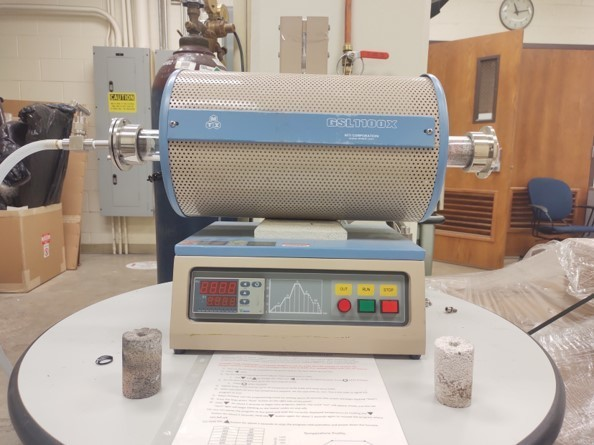
\includegraphics[width=0.45\linewidth]{mti-vacuum-furnace}%
\hfill
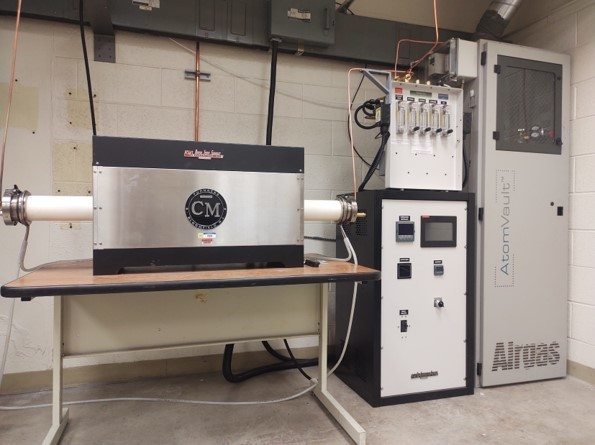
\includegraphics[width=0.45\linewidth]{cm-hydrogen-furnace}\\[-2pt]
{\tiny MTI Vacuum \hfill CM Hydrogen}
\end{minipage}

% ---------- COMPUTING ----------
\medskip\noindent\textbf{\textsc{Computing}}

\noindent
\begin{minipage}[t]{0.62\textwidth}\raggedright
\textbf{BYU HPC Cluster} (28K+ cores, 367~GPUs incl.\ H200/H100/A100,
SLURM).  No direct cost via fairshare scheduling.
Supports parallelized TC-Python CALPHAD sweeps and
BoTorch/GPyTorch surrogate training.
\end{minipage}\hfill
\begin{minipage}[t]{0.35\textwidth}
\centering
% HPC cluster image not available; text description sufficient.
\end{minipage}
\fi
%%% END UNUSED-FULL-DETAIL

% ============================================================================
%  APPENDIX 4: DATA MANAGEMENT AND SHARING PLAN (DMSP)
%  (NOT required at submission; required during award negotiation)
% ============================================================================
\newpage
\section*{Appendix 4: Data Management and Sharing Plan}
\label{app:dmsp}

\note{FOA \S IV.C: ``A Data Management and Sharing Plan (DMSP) is NOT
required as an appendix to the project narrative but it will be required
during award negotiation.''  This section is included for planning
purposes only.  You may request DMSP implementation costs in the budget.}

\guidance{When preparing the DMSP for award negotiation, it must address
(per FOA \S IV.C): (1) How FAIR principles will apply to datasets,
software, and models; (2) what will be released under open-source
licenses (specify SPDX identifiers); (3) how best practices in scientific
software development will be applied (see bssw.io).}

\textbf{1.\ Types of Data.} \flaime{} will generate: (i)~alloy composition
data (wt\%/at\% of Al, Mn, Cr, Zr via ICP-OES); (ii)~CALPHAD simulation
outputs (phase diagrams, Scheil--Gulliver curves, solidification parameters
from Thermo-Calc TCAl10/AM~Module); (iii)~powder characterization records
(PSD, SEM/EDS, flowability); (iv)~LPBF processing parameters (power, speed,
hatch spacing, layer thickness) and build metadata; (v)~mechanical properties
(YS, UTS, elongation per ASTM~E8/E8M) and microstructural images (SEM,
EBSD); and (vi)~BOFN/pKGFN model parameters, acquisition function logs, and
digital thread provenance records.

\textbf{2.\ Data Formats.} Tabular data will be stored in CSV/JSON with
documented JSON schemas. Large simulation arrays will use HDF5. Microscopy
images will be archived as lossless TIFF. ML models will be serialized in
ONNX for interoperability.

\textbf{3.\ Sharing and Preservation.} All experimental datasets will be
deposited on Zenodo and/or Figshare with DOIs within 12~months of
collection. The \flaime{} digital thread will be hosted on the American
Science Cloud (AmSC) per Genesis Mission requirements. Software
(BOFN/pKGFN engine, Honegumi tutorials) will be released on GitHub under
MIT/Apache-2.0 licenses, following bssw.io best practices.

\textbf{4.\ Access and Reuse.} Data and models will adhere to FAIR
principles. Datasets will carry rich README documentation and JSON
schemas for machine discoverability. Data licensed CC-BY-4.0; code
licensed MIT. Supply-risk
metadata (Helbig SRI scores, $\mathrm{HHI}_\text{production}$, $\mathrm{HHI}_\text{reserve}$, and 3-year average metal cost derived from the frozen USGS MCS~2024 dataset) will be linked to every composition record.

\textbf{5.\ Oversight.} The PI is responsible for DMSP compliance. Quarterly
data audits will be conducted throughout Phase~I. Budget provisions for data
curation, DOI registration, and AmSC hosting are included under Other
Direct Costs.

% ============================================================================
%  APPENDIX 5: SYNERGISTIC ACTIVITIES (Optional)
%  (1 page per senior/key person; does NOT count against narrative limit)
% ============================================================================
\newpage
\section*{Appendix 5: Synergistic Activities}
\label{app:synergistic}

\note{FOA \S IV.C: Optional. ``Each senior/key person has the option to
provide a one-page list of no more than five distinct examples of
synergistic activities that demonstrate the individual's professional
and scholarly activities that focus on the integration, transfer, and
creation of knowledge as related to the application.''  Total pages
$\leq$ number of senior/key personnel.}

\begin{enumerate}

\item \textbf{Self-Driving Laboratory Leadership \& Community Building.}
Serving as Guest Editor for \textit{npj Computational Materials} for the
``Self-Driving Labs for Chemistry and Materials Science'' collection
(2024--present) and lead author of the structural materials section of a
comprehensive \textit{Chemical Reviews} review on self-driving laboratories
(Tom et al., 2024). Lead author of a review on low-cost self-driving
laboratories introducing the ``Frugal Twin'' concept (Lo et al., 2024,
\textit{Digital Discovery}). Scientific Organizer for the Accelerate
Conference (2023, 2024)---a major self-driving laboratory conference with
hundreds of attendees. Solo-organized the Acceleration Consortium
Bayesian Optimization Hackathon (120 participants, 62 organizations,
14 countries).

\item \textbf{Open-Source Software \& Community Infrastructure.}
Contributed over 17,000 open-source code artifacts (15K commits, 1.5K
issues, 913 pull requests) spanning materials informatics, Bayesian
optimization, and laboratory automation. Creator of
\texttt{awesome-self-driving-labs}, a community-curated catalog of fully and
partially autonomous laboratories. Developer of Honegumi, an
interactive Bayesian optimization script generator for experimental
scientists (arXiv:2502.06815, under review), and xtal2png, a crystal-structure-to-image encoding
tool for generative modeling (JOSS, 2022). Served as Technical Consultant to
Meta for the v1.0 release of the Ax/BoTorch platform (Nov 2024--Jan 2025).
Over 350 self-driving lab demonstration kits deployed worldwide.

\item \textbf{Training \& Workforce Development.}
Delivered approximately 5,000 person-hours of self-driving laboratory
training to roughly 700 individuals across 62 organizations through
workshops, microcredential courses, and hackathons. Built the Acceleration
Consortium Development Lab from the ground up (\$600K in equipment, 500 line
items, 24 months). Developed over 200 hours of course content in robotics,
data science, and AI-driven experimental design.

\item \textbf{Standardization \& Open Science.}
Co-organizer of the annual NSF Pathways to Open-Source Ecosystems (POSE)
workshop (2024, 2025, 2026). Contributing to
Acceleration Consortium community standards for
self-driving laboratory interoperability and advancing FAIR data practices
for SDL datasets. Presenter at the
German-Canadian Materials Acceleration Centre (GCMAC) Summer School (2024,
2025) and Review Panelist for the NSF TIP Directorate (2026).

\item \textbf{Open Data Impact \& Domain Expertise.}
Creator of the MPTS-52 time-based dataset split, widely adopted in the
crystal structure generative AI community, and developer of the
Matbench-genmetrics framework for standardized evaluation of generative
models (JOSS, 2024). Completed a \$34K industry research contract with
Fehrmann Materials GmbH applying machine learning to joint strength and
ductility prediction in aluminum alloys. Maintains curated open datasets on
Zenodo and Figshare with documented community reuse.

\end{enumerate}

% ============================================================================
%  APPENDIX 6: TRANSPARENCY OF FOREIGN CONNECTIONS
%  (Required; does NOT count against narrative limit)
% ============================================================================
\newpage
\section*{Appendix 6: Transparency of Foreign Connections}
\label{app:foreign}

\required{FOA \S IV.C: Required for all applicants and subrecipients.
IHEs and non-profits: respond only to items marked with (*) in the
template.  DOE/NNSA labs and domestic government entities are exempt.
Use the template at
\url{https://www.energy.gov/ia/transparency-foreign-connections}
or provide equivalent information with signature, date, and certification
statement.  Include a separate disclosure for the applicant and each
proposed subrecipient.}

\instruct{If any partner is non-US (e.g., AMAZEMET, Poland), provide
complete foreign connections disclosure.  Route through BYU sponsored
programs office.}

Foreign-connections disclosure scope per FOA Appendix~6: BYU (lead applicant) and
Valimet, Inc.\ (Stockton, CA; funded subrecipient under BYU prime) are the two TFC-disclosing entities for this proposal. Completed
TFC disclosure and certification packets for BYU and Valimet are bundled
in the Field~12 submission package and prepared per the Valimet TFC
walkthrough (\texttt{outreach-drafts/letters/06-valimet-tfc-guide.md}).

\textbf{AMAZEMET Sp.\ z o.o.} (Warsaw, Poland) and \textbf{Thermo-Calc Software AB}
(Solna, Sweden) participate as \textbf{commercial vendors via BYU procurement}
(rePOWDER commissioning + training, and CALPHAD database/AM~Module licensing +
technical-staff support, respectively, in M\&S category~E). They
are not subrecipients, not Senior/Key Personnel, and not project team
members. Per FOA Appendix~6, TFC disclosure/certification is required only
for the applicant and proposed subrecipients; routine commercial vendor
procurements fall outside the TFC disclosure scope. AMAZEMET and Thermo-Calc
are therefore not separately disclosed in this Appendix~6.

% ============================================================================
%  APPENDIX 7: OTHER ATTACHMENTS
%  (Letters of Commitment, etc.; does NOT count against narrative limit)
% ============================================================================
\section*{Appendix 7: Other Attachments}
\label{app:other}

\required{FOA \S IV.C: ``Include the required Letters of Commitment and
any optional letters of collaboration or access.  You may also include
any needed elaboration to your responses to questions 1--6 on the `Other
Project Information' document or information not easily accessible to a
reviewer.  However, do not use this appendix to circumvent the page
limitations of the application.''}

\subsection*{A7.0 Phase~I Risk Register}
\label{app:risk-register}
Compact risk register referenced from the narrative \S\ref{sec:methods}
(Project Management, Risk \& Prior Work).
\begin{table}[H]
\centering\scriptsize
\setlength{\tabcolsep}{3pt}
\begin{tabularx}{\textwidth}{@{}p{0.18\textwidth}p{0.18\textwidth}p{0.10\textwidth}XX@{}}
\toprule
\textbf{Risk} & \textbf{Trigger} & \textbf{Owner} & \textbf{Mitigation} & \textbf{Off-ramp} \\
\midrule
(a) BYU rePOWDER atomizer not commissioned by M1 & AMAZEMET commissioning + AlSi10Mg baseline run not complete by end of M1 & PI + AMAZEMET vendor & Pre-negotiated remote engineering support; baseline production at AMAZEMET prior to shipment; parallel CALPHAD-only campaign continues & Shift initial 4--6 screening compositions to Valimet GA window~1 (compressed scope, 25\,kg lots) and a domestic backup ultrasonic atomizer; M1 deliverable redefined as software readiness only \\
\addlinespace[2pt]
(b) Valimet slips one production window & Quarterly window misses scheduled date by $>$2 weeks & Valimet's technical manager + PI & Reserved priority slots in SOW; 10-business-day rework/scope-substitution clause; remaining 5 windows resequenced & Drop one of the 6 runs; reallocate the remaining Valimet balance toward 2 extra ultrasonic-atomized BYU lots for the affected composition family \\
\addlinespace[2pt]
(c) First-print density below 99\% relative threshold after $\geq$5 build attempts & Density cubes (node~6c) fail $<$99\% on Sobol initial designs across $\geq$5 compositions & PI + Spear lab (node~5b) & Parameter-finding sub-loop with AM~Module (node~2b)-recalibrated absorptivity; tighten powder PSD acceptance (node~4); expand laser-power/scan-speed grid & Restrict initial campaign to AlSi10Mg-adjacent compositions known to print; defer L1$_2$ family to Phase~II \\
\addlinespace[2pt]
(d) Valimet TFC / subaward packet not complete by proposal lock & Packet not signed/returned by submission day~$-$2 & PI + BYU OSP & Prefilled packet (\texttt{outreach-drafts/letters/01-valimet-loc-prefilled.md}) + role-based 7-day walkthrough; weekly check-in with Valimet contracts & Submit with reduced Valimet scope (LoCol-only access agreement) and request post-award subaward issuance per FOA \\
\addlinespace[2pt]
(e) pKGFN sample-efficiency at-or-below standard-BO baseline & Pre-registered ablation at $\sim$50 evaluated points shows pKGFN AF $<$1.5$\times$ vs.\ standard BO & PI & Switch live loop to standard BO with the same SAASBO sparse-GP surrogate; pKGFN demoted to offline / Phase~II refinement; AF report frames result honestly per pre-registered time-ledger & Continue campaign with standard BO; Phase~I AI-advantage claim narrowed to discovery-yield + mineral-burden gates rather than acceleration factor \\
\addlinespace[2pt]
(f) AM~Module calibration drift & Predicted-vs-measured melt-pool depth/width error $>$25\% on $\geq$3 calibration compositions & PI + Thermo-Calc's account manager & Fixed calibration composition set (AlSi10Mg + Al-Mn-Cr-Zr ``Alloy~C''); recalibration cadence after each Valimet window; absorptivity update via melt-pool cross-sections (node~6a) & Demote AM~Module (node~2b) from acquisition-loop node to offline advisory model; rely on \texttt{pycalphad}/TC-PRISMA + experimental density gate (node~7a) alone \\
\addlinespace[2pt]
(g) AMAZEMET rePOWDER international shipping/customs delay & Crate not cleared US customs by 2026-05-15 (target dock-to-BYU 2026-04-30 + 2-week customs buffer) & PI + AMAZEMET vendor + BYU shipping/receiving & Pre-cleared HTS classification at quote stage; INCOTERMS DAP Provo with broker-of-record on file; weekly tracking with AMAZEMET logistics; AlSi10Mg baseline produced at AMAZEMET Warsaw and shipped as finished powder ahead of equipment & Push M1 milestone by up to 6~weeks (absorbed in 9-month PoP via Sobol-only CALPHAD pre-runs); first 4--6 BYU-side compositions produced at Valimet GA window~1 instead; FLAIME loop continues on simulation + Valimet powder \\
\bottomrule
\end{tabularx}
\end{table}

% ---------------------------------------------------------------------------
%  QUICK-REFERENCE GUIDE FOR COLLABORATORS
% ---------------------------------------------------------------------------
\medskip
\noindent\fbox{\parbox{\dimexpr\textwidth-2\fboxsep-2\fboxrule}{%
\small\textbf{Quick-Reference: Letter Types Required by this FOA
(DE-FOA-0003612)}\\[3pt]
The RFA specifies \textbf{two} types of letters. \emph{Letters of
recommendation / endorsement are \underline{not} allowed.}\\[4pt]
%
\begin{tabular}{@{}p{0.28\textwidth}p{0.68\textwidth}@{}}
\toprule
\textbf{Letter of Commitment} &
  Required from every institution \textbf{participating as a team member}
  (including the lead).
  Must be current, signed, and dated by a \textbf{person authorized to
  commit the institution to a legally binding agreement}.
  Maximum \textbf{one page}.
  Describes the nature of the institution's involvement. \\[3pt]
\textbf{Letter of Collaboration or Access} &
  Optional; from collaborators or institutions providing access to data,
  models, software, equipment, and/or facilities.
  Must follow a \textbf{strict 2-sentence format} (see template below).
  Must \underline{not} read as a recommendation or endorsement.
  No page limit stated, but brevity is expected. \\
\bottomrule
\end{tabular}\\[4pt]
\textit{All letters go in Appendix~7 (Other Attachments).
All letters may be addressed ``To Whom It May Concern.''}%
}}

% ---------------------------------------------------------------------------
%  WHO NEEDS WHAT
% ---------------------------------------------------------------------------
\medskip
\noindent\textbf{Letters needed for this proposal:}

\begin{enumerate}[leftmargin=*,nosep]\small
  \item \textbf{BYU} (lead institution) --- Letter of Commitment (signed by
        authorized university official, e.g.\ SPO or Dean)
  \item \textbf{Valimet, Inc.} (funded subrecipient under BYU prime) ---
        Letter of Commitment (BYU subaward; $\geq$20\% Valimet entity
        cost share per FOA \S II.B; signed by authorized representative;
        prefilled letter at \texttt{outreach-drafts/letters/01-valimet-loc-prefilled.md})
  \item \textbf{AMAZEMET Sp.\ z o.o.} (commercial vendor / BYU procurement)
        --- Letter of Collaboration (strict 2-sentence format; rePOWDER
        commissioning, training, and engineering support procured by BYU as
        a commercial vendor; signed by authorized representative)
  \item \textbf{University of Utah / Prof.\ Ashley Spear} --- Letter of
        Collaboration or Access (Metal 3D Printing Core Facility access
        at published recharge rate; confirmed by PI 2026-04-21)
  \item \textbf{Alik Nielsen (UofU Metal 3D Printing Core Facility, Primary
        Operator)} --- Letter of Collaboration or Access (build scheduling
        and assisted-service operation)
  \item \textbf{Thermo-Calc Software AB} (commercial vendor / BYU procurement)
        --- Letter of Collaboration (strict 2-sentence format; CALPHAD
        databases, AM~Module licenses \& technical-staff support procured by
        BYU as a commercial vendor; signed by authorized representative)
  \item \textbf{3D Powder Tech} --- Letter of Collaboration or Access
        (backup LPBF capacity; 2-sentence format)
  \item \textbf{Meta / BoTorch team} --- Letter of Collaboration or Access
        (BoTorch ecosystem; 2-sentence format)
  \item \textbf{Prof.\ Brian Jensen (BYU ME Chair)} --- Letter of Commitment
        (teaching relief + up to \$50K departmental cost share toward
        co-located BYU LPBF printer)
  \item \textbf{Prof.\ Taylor Sparks (UofU)} --- Letter of Collaboration or Access
        (advisory role; 2-sentence format) \textit{[if applicable]}
\end{enumerate}

\medskip
\noindent\textbf{Advisory Letters of Collaboration} \textit{(received;
ordered by relevance to the FLAIME narrative --- AM process science,
Al-alloy / CALPHAD expertise, and AI-for-materials methodology):}

\begin{enumerate}[leftmargin=*,nosep,start=11]\small
  \item \textbf{Prof.\ Anthony D.\ Rollett (Carnegie Mellon)} --- Letter of
        Collaboration or Access (advisory: AM process science, melt-pool
        physics, and AM~Module calibration credibility)
  \item \textbf{Prof.\ Aaron P.\ Stebner (Georgia Tech)} --- Letter of
        Collaboration or Access (advisory: AI-for-AM, ML-driven qualification,
        and ASTM~E8/E8M specimen workflows)
  \item \textbf{Prof.\ Yongho Sohn (UCF)} --- Letter of Collaboration or
        Access (advisory: Al-alloy CALPHAD-aligned diffusion and
        microstructure analysis)
  \item \textbf{Prof.\ Rajiv S.\ Mishra (UNT)} --- Letter of Collaboration or
        Access (advisory: high-entropy / multi-principal-element AM alloys
        and ICME)
  \item \textbf{Prof.\ Lianyi Chen (Wisconsin)} --- Letter of Collaboration
        or Access (advisory: in-situ melt-pool dynamics and high-speed AM
        imaging)
  \item \textbf{Prof.\ Frank E.\ Pfefferkorn (Wisconsin)} --- Letter of
        Collaboration or Access (advisory: laser AM process science and
        thermal modeling)
  \item \textbf{Prof.\ Timothy A.\ Horn (NC State)} --- Letter of
        Collaboration or Access (advisory: NCSU CAMAL fabrication services
        and powder-handling safety screening for distributed validation)
  \item \textbf{Prof.\ Francisco Medina (UTEP)} --- Letter of Collaboration
        or Access (advisory: UTEP W.M.\ Keck Center for 3D Innovation LPBF
        cross-validation prints)
  \item \textbf{Prof.\ Craig A.\ Brice (Colorado School of Mines)} ---
        Letter of Collaboration or Access (advisory: LPBF specimen
        fabrication and cross-printer build-metadata exchange)
  \item \textbf{Prof.\ Nathan B.\ Crane (BYU ME)} --- Letter of Collaboration
        or Access (advisory: internal BYU AM faculty; specimen handling,
        post-processing, and lab-scale process integration)
\end{enumerate}

\guidance{Collect signed, dated letters on official letterhead.
Confirm the authorized signatory for each institution (Commitment letters
require someone who can bind the institution; Collaboration letters may be
from the individual collaborator).  PDF format preferred.  Letters of
Commitment count toward the list in the FAQ: ``a letter of commitment,
signed by a person authorized to commit the participating institution to a
legally binding agreement, is required from each institution participating
as a team member on the proposal.  This includes the lead institution''
(FAQ, p.9--10).}

% ---------------------------------------------------------------------------
%  TEMPLATE: LETTER OF COLLABORATION (STRICT 2-SENTENCE FORMAT)
% ---------------------------------------------------------------------------
\bigskip
\noindent\textbf{\large Draft Letter Templates}

\medskip
\noindent\rule{\textwidth}{0.4pt}\\
\textbf{Type A: Letter of Collaboration or Access} \textit{(strict 2-sentence format per FOA p.65)}
\smallskip

\begin{quote}\small
\textbf{{[}Institutional Letterhead{]}}\\[4pt]
{[}Date{]}\\[6pt]
Dear Prof.\ Sterling G.\ Baird:\\[4pt]
If your application entitled, ``\projecttitle{},'' is selected for
funding under DE-FOA-0003612, it is my intent to collaborate in this
research by {[}\emph{one sentence describing what the collaborator
offers to do or provide}{]}.
Thank you for the opportunity to participate.\\[12pt]
Sincerely,\\[4pt]
{[}Name{]}\\
{[}Title{]}\\
{[}Department / Organization{]}\\
{[}Street Address{]}\\
{[}City, State ZIP{]}\\
{[}Institutional Email{]}\\
{[}Phone{]}
\end{quote}

\medskip
\noindent\rule{\textwidth}{0.4pt}\\
\textbf{Type B: Letter of Commitment} \textit{(from funded team member institutions; max 1 page)}
\smallskip

\begin{quote}\small
\textbf{{[}Institutional Letterhead{]}}\\[4pt]
{[}Date{]}\\[6pt]
To Whom It May Concern:\\[4pt]
This letter confirms the commitment of {[}Organization{]} to participate as a
funded partner in the proposed project ``\projecttitle{}''
(DE-FOA-0003612) with a subaward of \${[}amount{]}.\\[4pt]
{[}Organization{]} will {[}\emph{specific deliverables, named personnel,
\% effort, schedule, and resources committed}{]}.\\[4pt]
The scope of work, budget, and timeline are detailed in the attached subaward
budget and will be executed in accordance with the project milestones
described in the Project Narrative.\\[4pt]
{[}Name{]}, {[}Title{]}, is authorized to commit {[}Organization{]} to this
legally binding agreement.\\[12pt]
Sincerely,\\[4pt]
{[}Name{]}\\
{[}Title (authorized signatory){]}\\
{[}Organization{]}\\
{[}Street Address{]}\\
{[}City, State ZIP / Country{]}\\
{[}Institutional Email{]}\\
{[}Phone{]}
\end{quote}

% ---------------------------------------------------------------------------
%  PRE-DRAFTED LETTERS (collaboration/access, 2-sentence format)
% ---------------------------------------------------------------------------
\bigskip
\noindent\rule{\textwidth}{0.4pt}\\
\textbf{\large Pre-Drafted Letters} \textit{(ready for collaborator review and signature)}

% ---- Brian Jensen ----
\includepdf[pages=-,pagecommand={\thispagestyle{plain}}]{appendix-7-letters/brian-jensen-byu-loc.pdf}

% ---- Ashley Spear ----
\includepdf[pages=-,pagecommand={\thispagestyle{plain}}]{appendix-7-letters/ashley-spear-uofu-loc.pdf}

% ---- Alik Nielsen ----
\includepdf[pages=-,pagecommand={\thispagestyle{plain}}]{appendix-7-letters/alik-nielsen-uofu-loc.pdf}

% ---- Thermo-Calc ----
\includepdf[pages=-,pagecommand={\thispagestyle{plain}}]{appendix-7-letters/thermo-calc-letter-of-collaboration.pdf}

% ---- BYU Student Commitment Letters ----
\includepdf[pages=-,pagecommand={\thispagestyle{plain}}]{appendix-7-letters/student-commitment-letters/madsen-byu-loc.pdf}
\includepdf[pages=-,pagecommand={\thispagestyle{plain}}]{appendix-7-letters/student-commitment-letters/gage-erickson-byu-loc.pdf}
\includepdf[pages=-,pagecommand={\thispagestyle{plain}}]{appendix-7-letters/student-commitment-letters/seth-leavitt-byu-loc.pdf}

% ---- 3D Powder Tech ----
\clearpage
\textit{Letter of Collaboration or Access --- 3D Powder Tech (Backup LPBF):}

\begin{quote}\small
\textbf{{[}3D Powder Tech Letterhead{]}}\\[4pt]
{[}Date{]}\\[6pt]
Dear Prof.\ Sterling G.\ Baird:\\[4pt]
If your application entitled, ``\projecttitle{},'' is selected for
funding under DE-FOA-0003612, it is my intent to collaborate in this
research by providing backup laser powder bed fusion printing capacity for
Al alloy specimens when additional throughput or alternative build
parameters are required beyond the primary LPBF facility.
Thank you for the opportunity to participate.\\[12pt]
Sincerely,\\[4pt]
{[}Name, Title{]}\\
3D Powder Tech\\
{[}Address{]}\\
{[}email{]}\\
{[}phone{]}
\end{quote}

% ---- Meta / BoTorch ----
\includepdf[pages=-,pagecommand={\thispagestyle{plain}}]{appendix-7-letters/meta-letter-of-collaboration.pdf}

% ---- Taylor Sparks (optional) ----
\clearpage
\textit{Letter of Collaboration --- Prof.\ Taylor Sparks (UofU, Advisory):}
\textit{{[}Include only if Prof.\ Sparks has a defined advisory role.{]}}

\begin{quote}\small
\textbf{{[}University of Utah, Materials Science \& Engineering Letterhead{]}}\\[4pt]
{[}Date{]}\\[6pt]
Dear Prof.\ Sterling G.\ Baird:\\[4pt]
If your application entitled, ``\projecttitle{},'' is selected for
funding under DE-FOA-0003612, it is my intent to collaborate in this
research by providing advisory expertise in high-throughput materials
discovery and data-driven alloy design methodologies.
Thank you for the opportunity to participate.\\[12pt]
Sincerely,\\[4pt]
Taylor~D.~Sparks, Ph.D.\\
Professor\\
Department of Materials Science and Engineering\\
University of Utah\\
122 S Central Campus Dr, Salt Lake City, UT 84112\\
{[}email@utah.edu{]}\\
{[}phone{]}
\end{quote}

% ---- Printing Partner (Multi-Site Validation) ----
\clearpage
\textit{Letter of Collaboration or Access --- Printing Partner (Multi-Site Validation):}

\begin{quote}\small
\textbf{{[}Organization Letterhead{]}}\\[4pt]
{[}Date{]}\\[6pt]
Dear Prof.\ Sterling G.\ Baird:\\[4pt]
If your application entitled, ``\projecttitle{},'' is selected for
funding under DE-FOA-0003612, it is my intent to collaborate in this
research by accepting a batch of gas-atomized powder for one or more
validated \flaime{} alloy compositions, printing specimens on our
{[}LPBF/DED/Binder Jet{]} system under our standard parameters, and
returning at least one sample per composition (with associated build
metadata: scan settings, build log, post-processing parameters) so that
alloy performance can be cross-validated across printers and process
conditions rather than localized to a single machine.
Thank you for the opportunity to participate.\\[12pt]
Sincerely,\\[4pt]
{[}Name{]}\\
{[}Title{]}\\
{[}Organization{]}\\
{[}Address{]}\\
{[}Email{]}\\
{[}Phone{]}
\end{quote}

% ---------------------------------------------------------------------------
%  ADVISORY LETTERS OF COLLABORATION (received signed PDFs; ordered by
%  narrative relevance: AM process science, Al-alloy / CALPHAD, AI-for-AM)
% ---------------------------------------------------------------------------
\bigskip
\noindent\rule{\textwidth}{0.4pt}\\
\textbf{\large Advisory Letters of Collaboration --- Distributed
Validation Network} \textit{(signed; print partners offering
fabrication/characterization access; ordered by relevance to the
FLAIME narrative)}

% ---- Tony Rollett (CMU) ----
\includepdf[pages=-,pagecommand={\thispagestyle{plain}}]{appendix-7-letters/distributed-validation-network/tony-rollet-cmu-loc.pdf}

% ---- Sneha Prabha Narra (CMU) ----
\includepdf[pages=-,pagecommand={\thispagestyle{plain}}]{appendix-7-letters/distributed-validation-network/sneha-prabha-narra-cmu-loc.pdf}

% ---- Aaron Stebner (GA Tech) ----
\includepdf[pages=-,pagecommand={\thispagestyle{plain}}]{appendix-7-letters/distributed-validation-network/aaron-stebner-gatech-loc.pdf}

% ---- Yongho Sohn (UCF) ----
\includepdf[pages=-,pagecommand={\thispagestyle{plain}}]{appendix-7-letters/distributed-validation-network/yongho-sohn.pdf}

% ---- Rajiv Mishra (UNT) ----
\includepdf[pages=-,pagecommand={\thispagestyle{plain}}]{appendix-7-letters/distributed-validation-network/rajiiv-mishra-unt-loc.pdf}

% ---- Lianyi Chen (Wisconsin) ----
\includepdf[pages=-,pagecommand={\thispagestyle{plain}}]{appendix-7-letters/distributed-validation-network/lianyi-chen-wisc-loc.pdf}

% ---- Frank Pfefferkorn (Wisconsin) ----
\includepdf[pages=-,pagecommand={\thispagestyle{plain}}]{appendix-7-letters/distributed-validation-network/frank-pfefferkorn-wisc-madison-loc.pdf}

% ---- Tim Horn (NC State) ----
\includepdf[pages=-,pagecommand={\thispagestyle{plain}}]{appendix-7-letters/distributed-validation-network/tim-horn-ncsu-loc.pdf}

% ---- Frank Medina (UTEP) ----
\includepdf[pages=-,pagecommand={\thispagestyle{plain}}]{appendix-7-letters/distributed-validation-network/frank-medina-utep-loc.pdf}

% ---- Craig Brice (Colorado School of Mines) ----
\includepdf[pages=-,pagecommand={\thispagestyle{plain}}]{appendix-7-letters/distributed-validation-network/craig-brice-mines-loc.pdf}

% ---- Nathan Crane (BYU ME) ----
\includepdf[pages=-,pagecommand={\thispagestyle{plain}}]{appendix-7-letters/distributed-validation-network/nathan-crane-letter-of-collaboration.pdf}

% ---------------------------------------------------------------------------
%  PRE-DRAFTED LETTERS OF COMMITMENT (funded subrecipients)
% ---------------------------------------------------------------------------
\bigskip
\noindent\rule{\textwidth}{0.4pt}\\
\textbf{Letters of Commitment (Funded Subrecipients)}

% ---- Valimet ----
\includepdf[pages={2},pagecommand={\thispagestyle{plain}}]{appendix-7-letters/funded-subrecipients/valimet-letter-of-commitment.pdf}

% ---- AMAZEMET ----
\clearpage
\textit{Letter of Collaboration --- AMAZEMET Sp.\ z o.o.\ (Ultrasonic
Atomization; Commercial Vendor / BYU Procurement):}

\begin{quote}\small
\textbf{{[}AMAZEMET Sp.\ z o.o.\ Letterhead{]}}\\[4pt]
{[}Date{]}\\[6pt]
To Whom It May Concern:\\[4pt]
If the application entitled, ``\projecttitle{},'' is selected for funding
under DE-FOA-0003612, it is my intent to collaborate in this research by
providing rePOWDER ultrasonic-atomization commissioning, on-site operator
training, and ongoing remote engineering support to Brigham Young
University as a commercial vendor procurement under the BYU prime award.
Thank you for the opportunity to participate.\\[12pt]
Sincerely,\\[4pt]
{[}Name{]}, {[}Title{]}\\
AMAZEMET Sp.\ z o.o.\\
Al.\ Jana Paw{\l}a~II 27, 00-867 Warsaw, Poland\\
{[}email@amazemet.com{]}\\
{[}phone{]}
\end{quote}

% ============================================================================
%  APPENDIX 8: EXTENDED TECHNICAL DETAILS & SUPPORTING FIGURES
%  (Supporting material offloaded from narrative to respect 5-page limit;
%   does NOT count against narrative limit.)
% ============================================================================
% Appendix 8 ACTIVATED to absorb narrative detail (BOFN architecture,
% mineral-lean baselines, LPBF funnel arithmetic) so the narrative meets
% the FOA 5-page limit.  Cross-referenced from \S3 (Methods) and
% \S\ref{sec:gates} (Decision Gates).
\newpage
\section*{Appendix 8: Extended Technical Details \& Supporting Figures}
\label{app:extended}

\note{Material offloaded from the Project Narrative to comply with the
FOA 5-page narrative limit.  Cross-referenced from \S1 (Background),
\S3 (Methods), and \S\ref{sec:gates} (Decision Gates).}

\subsection*{A8.1 BOFN/pKGFN Architecture, Surrogate, and Ablation Plan (Activity~1 detail)}
\label{app:a81-bofn}

The \flaime{} optimizer is a Bayesian Optimization over Function
Networks (\bofn{}) directed acyclic graph
(DAG; Fig.~\ref{fig:flaime-dag})~\cite{sundar_2025_s4357802,paramore_2025_jactamat} covering
Thermo-Calc AM~Module simulation, powder, LPBF, and mechanical-response nodes.
The \emph{partial} Knowledge Gradient for Function
Networks (pKGFN)~\cite{buathong_2023_23110214,buathong_2025_25061145}
is the acquisition function that selects which node and inputs to
evaluate next in a cost-aware manner: ``partial'' because not every
node is evaluated at each iteration (e.g., a Thermo-Calc AM~Module
query can be run without triggering an expensive tensile test),
``knowledge gradient'' because the decision maximizes the expected
improvement in the global objective per unit cost across fidelities
ranging from Thermo-Calc AM~Module simulation to full
powder dosing, atomization, LPBF printing, and tensile testing, and
``network'' because the DAG structure---where
each node's output feeds downstream nodes---is
exploited to propagate information efficiently.
A mineral-burden node (analytical, noise-free) exposes two cost-weighted
scalars: $\mathrm{MBS}_{\text{lin}}{=}\sum_{i\neq\mathrm{Al}}\mathrm{NIR}_i(c_i/c_{\mathrm{Al}})x_i$
(Gate~G3a Sc-elimination) and $\mathrm{CMDRI}_{\text{log}}{=}\sum_{i\neq\mathrm{Al}}\mathrm{NIR}_i\log_{10}(1+c_i/c_{\mathrm{Al}})x_i$
(continuous BOFN objective and G3b backfill ceiling vs.\ AlSi10Mg;
Table~\ref{tab:gates}), with USGS MCS~2024 NIR~\cite{usgs_mcs_2024}
and 2022--2024 prices frozen at M1 (2025 USGS list adds Al/Si/Cu; base
Al excluded). Graedel~\cite{graedel_2012_es203534}, Helbig~\cite{mulukutla_2024_ssrn4968},
ESSENZ~\cite{cimprich_2019_jiec1286}, and $\mathrm{HHI}_{\text{prod/res}}$
enter as digital-thread reporting metadata/contextual BOFN features
(not gate multipliers), per the multi-axis framework of Baird~\&~Sparks~\cite{titirici_2022_roadmap}.
Preliminary pKGFN convergence
(Fig.~\ref{fig:pipeline}) and active CALPHAD evaluation on BYU
HPC confirm readiness.

\textbf{Joint Acquisition with GA Inner Solver.}
The 15-element palette (Al + Mn, Cr, Zr, Mg, Si, Cu, Ti, Fe, Ni, Ce, Sc, Li,
Er, Zn, Sn) defines the \emph{outer feasibility envelope} (per-element
upper bounds, baseline-family priors, USGS-derived mineral-burden
context). The \emph{live} pKGFN BO loop in Phase~I jointly optimizes the
\textbf{full 15-element bounded composition vector + 2--3 process variables} (laser
power $P\in[100,400]$\,W, scan speed $v\in[200,2000]$\,mm/s, hatch
spacing $h\in[80,150]$\,\textmu m, with layer thickness fixed at
30\,\textmu m for the Aconity MIDI 200\,W/400\,W heads). SAASBO's
sparsity prior automatically deactivates non-contributing elements per
family
(Al--Mn--Cr--Zr-anchored, Al--Zr L1$_2$-anchored, and a Mn/Cr/Zr-lean
family; \S A8.4). The outer generator's active-subspace assignment is
\textbf{pooled across families} via a single shared SAASBO sparse-GP
surrogate (the per-family designation is a soft prior on element
weights, not a partition); the active subspace is rotated only when the
posterior pareto-front along the mineral-burden / printability /
strength axes saturates ($<$5\% improvement over a 16-acquisition
window) or when an off-ramp triggers (Appendix~7), so surrogate state
carries forward across rotations rather than being reset. This
matches the dimensionality range where pKGFN/BOFN
sample-efficiency is empirically demonstrated~\cite{buathong_2023_23110214,buathong_2025_25061145}
and avoids extrapolating to a joint $\sim$15-D composition $\times$ multi-process surrogate
that is not benchmarked in the literature. We pre-register a Phase~I
\textbf{ablation comparing pKGFN vs.\ standard BO} at the actual 4--6+2--3
dimensionality on simulator surrogates plus the first $\sim$50 experimental
points; the AI Acceleration Factor in \S\ref{sec:gates} is reported against
this same dimensionality.
The compositional decision space is a bounded continuous vector with
simplex (mass-balance) and per-element box constraints; the 15-element
palette spans a candidate envelope of
$\sum_{k=2}^{8}\binom{\elementcount}{k}=\subsystemcount{}$
element-combination subsystems from which the outer generator selects
the active subspace --- this count describes the candidate envelope, not
the dimensionality of the BO problem solved at each acquisition.
Pending evaluations are handled via fantasy samples so the acquisition
stays asynchronous across CALPHAD, HPC, and experimental queues; a
Sobol quasi-random design (24--40 initial points spanning baseline
families, simplex corners, and a constrained design over the active
subspace) kickstarts the campaign before pKGFN takes over.
%
\emph{CALPHAD function-network nodes (explicit intermediate nodes, not
contextual features).}
\texttt{pycalphad}~\cite{otis_2024_97810035} ($\sim$ms--sec/eval; license-free
batch evaluation of phase fractions and CSI), TC-Python + TCAl10 Scheil
and TC-PRISMA ($\sim$1--5\,CPU-min/eval), and the Thermo-Calc AM~Module
($\sim$0.5--2\,CPU-hr/eval; printability, melt-pool) sit as three
\textbf{explicit intermediate function-network nodes} with defined outputs,
Gaussian noise models, and per-call cost estimates. pKGFN selects per
candidate which node(s) to evaluate under a cost budget; a missing-node
observation is handled by partial-evaluation acquisition (downstream
nodes consume CALPHAD outputs as upstream inputs and propagate
posterior uncertainty when a CALPHAD parent is unobserved). Specifically,
the powder/atomization node consumes phase fraction + CSI from
\texttt{pycalphad}; the LPBF node consumes printability score and
melt-pool geometry from AM~Module; the mechanical-response node consumes
the predicted as-printed microstructure from TC-PRISMA. AM~Module
predictions map to Aconity MIDI parameters and are reciprocally
calibrated by FLAIME prints. For Phase~I we commit to a single
surrogate family, \textbf{SAASBO sparse-GP priors}~\cite{eriksson_2021_21030034}
appropriate for the 4--6+2--3 dimensionality and small initial design;
deep-kernel (SVDKL) extensions are deferred to Phase~II pending
in-domain evidence of gain. The mineral-burden score is a first-class
BOFN objective node~\cite{bocklund_2020_20011161,sabanzagil_2025_s4358802}.

\subsection*{A8.2 CALPHAD Partial-Evaluation Nodes (Activity~1 detail)}
The three CALPHAD tools sit as \emph{parallel} partial-evaluation nodes
in the function network, not as a sequential cascade; pKGFN decides
per-candidate which node(s) to query under the cost budget.
\textbf{pycalphad (cheap; $\sim$ms--sec/eval).}
\texttt{pycalphad}~\cite{otis_2024_97810035} computes phase
fractions and CSI as the \emph{outputs of the cheap upstream node},
which are then consumed as inputs by the powder/atomization,
LPBF, and mechanical-response downstream nodes (consistent with
A8.1; not used as side-information ``contextual features''). Being
license-free and Python-native, it is the only CALPHAD option that
can be called at the GA inner-solver's evaluation rate without
contending for the TC license pool, and it makes the cheap upstream
node reproducible without a Thermo-Calc seat. pycalphad uses open
TDBs (not the proprietary TCAL10); pKGFN's partial-evaluation
acquisition propagates posterior uncertainty when only the cheap
node has been observed, and selectively triggers a TCAl10/AM~Module
evaluation when the value-of-information warrants it.
Scheil solidification and the mineral-burden score are computed
by other nodes: Scheil is computed inside the TC-Python node, and
the mineral-burden score is a first-class BOFN objective node~\cite{bocklund_2020_20011161}.
\textbf{TC-Python + TCAl10 (mid; $\sim$1--5\,CPU-min/eval):}
Scheil with back-diffusion and TC-PRISMA precipitation kinetics.
\textbf{Thermo-Calc AM~Module (costly; $\sim$0.5--2\,CPU-hr/eval):}
printability maps, melt-pool geometry, and Scheil at LPBF cooling rates
($10^{4}$--$10^{6}$~K/s) (see Fig.~\ref{fig:baseline-supp})---many of these parameters map directly to
tunable settings on the Aconity MIDI's open-parameter
architecture---inform candidate viability before atomization.  FLAIME
prints reciprocally calibrate the AM~Module's aluminum absorptivity
(Appendix~2), and AM~Module simulations can be re-run post-improvement
and replaced into the surrogate to improve the campaign itself.
\textbf{Scalability.} For expensive prediction nodes in 6+ component
spaces, SAASBO~\cite{eriksson_2021_21030034} identifies sparse relevant
subspaces (scaling as $n^{3}$ in data points, limiting to hundreds of
evaluations---appropriate for the experimental budget). Deep-kernel
(SVDKL~\cite{sabanzagil_2025_s4358802}) extensions are deferred to
Phase~II pending in-domain evidence of gain (consistent with A8.1).
Periodic diversity-enforcing re-focusing---based on
posterior uncertainty decay over evaluated regions---prevents premature
convergence to a narrow region of composition space.

\begin{figure}[!tb]
  \centering
  \fbox{\begin{minipage}[c][1.8in][c]{0.6\linewidth}
    \centering\scriptsize
    \textit{Placeholder:} \texttt{example-image-a} (Al--Mn--Cr--Zr and Al--Zr CALPHAD from TCAl10/AM~Module).
  \end{minipage}}
  \caption{Baseline-comparator CALPHAD output for Al--Mn--Cr--Zr and Al--Zr using TCAl10/AM~Module. The AM~Module workflow is already validated for the AlSi10Mg baseline (Fig.~\ref{fig:baseline-supp}; Thermo-Calc~AB); the anchor-system runs (Al-5Mn-0.8Cr-0.5Zr ``Alloy~C'' and Al-1.5Zr) are scheduled next per the Thermo-Calc-provided composition list.}
  \label{fig:anchor-calphad}
\end{figure}

\subsection*{A8.3 Experimental Pipeline Detail (Activity~2)}

\subsubsection*{A8.3.1 LPBF print funnel and machine-hour budget}
\label{app:a83-funnel}

LPBF printing is performed at the University of Utah (Prof.\ Ashley
Spear's lab, Aconity MIDI; 3D~Powder Tech backup) under an explicit
\textbf{print funnel}: $\sim$160 atomized compositions $\to$ $\sim$80
density cubes ($\geq$99\% relative density gate) $\to$ $\sim$40
ASTM~E8/E8M sub-size tensile builds on the top quartile $\to$
top-3 elevated-temperature validation builds (three temperatures, App.~3)
for L1$_2$ stability. Each stage is cost-aware,
partial-evaluation-gated, and early-stoppable. Stage-gating
arithmetic: at the Aconity MIDI's 170\,mm $\varnothing$ build plate
($\sim$22{,}700\,mm$^{2}$ usable area), $\sim$10--16 density cubes per
plate and $\sim$4--6 ASTM~E8 sub-size bars per plate set the
plate-throughput floor; the funnel sizes ($\sim$160 / $\sim$80 / $\sim$40)
are derived from the BYU--UofU machine-hour budget at the UofU
\$120/hr Aconity MIDI rate (App.~3 facilities cost). Sub-size ASTM~E8/E8M
specimens (100\,mm length instead of 200\,mm) are standard in LPBF
screening with YS/UTS within
$\sim$5\%~\cite{paraschiv_2023_ma16144930,wang_2020_17452759};
elongation per ASTM~E8/E8M~\cite{astm_2024_e8e8m}.  Preliminary
AlSi10Mg tensile data (Fig.~\ref{fig:tensile}) establishes the pipeline
baseline before campaign launch.

\subsubsection*{A8.3.2 AMAZEMET rePOWDER operational detail}
\label{sec:amazemet-detail}

The AMAZEMET rePOWDER ultrasonic atomizer includes an induction crucible
module. Elemental-powder mixtures are loaded into machined high-purity
aluminum crucibles that jointly serve as the bulk Al contribution, the
``dispense vial'', and a compaction die (see Appendix~2). A press-fit lid
compacts the powder charge, reducing oxidation and shortening the time to
a homogenized melt (improved wettability), which in turn limits
evaporative loss of volatile additions; time--temperature curves are
logged per run to track retention.

\begin{figure}[!tb]
  \centering
  \begin{tabular}{@{}cc@{}}
    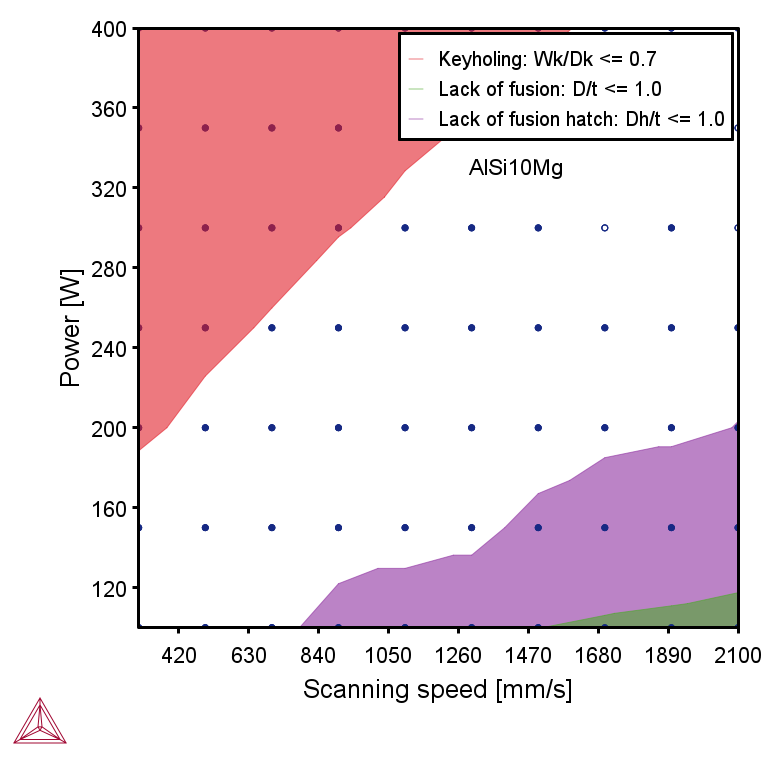
\includegraphics[width=0.42\linewidth]{../figures/thermo-calc-am-module-prelim-results/AlSi10Mg-printability-map.png} &
    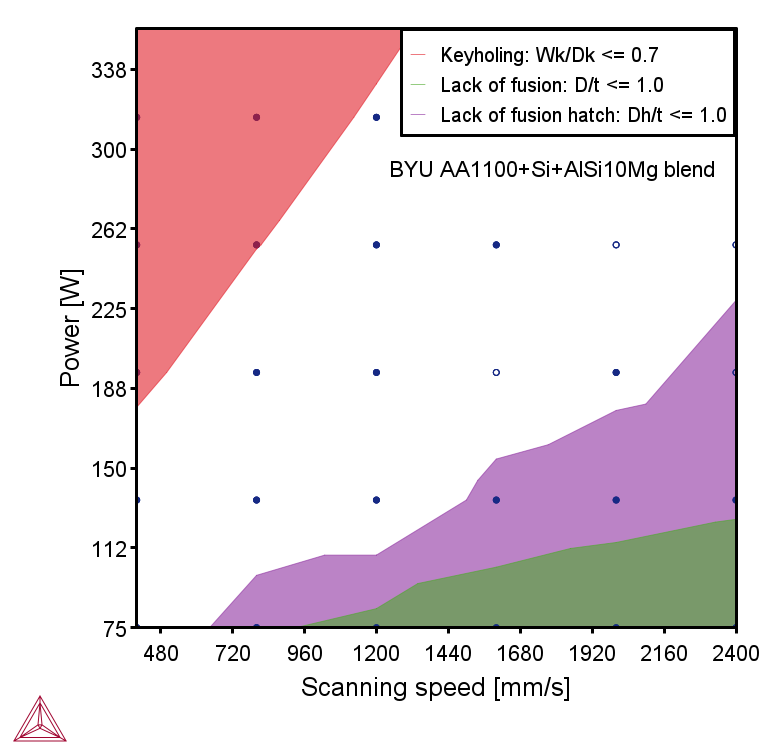
\includegraphics[width=0.42\linewidth]{../figures/thermo-calc-am-module-prelim-results/BYU-AA1100-Si-AlSi10Mg-blend-printability-map.png} \\
    {\scriptsize (a) Stock AlSi10Mg printability map} & {\scriptsize (b) BYU AA1100+Si+AlSi10Mg blend printability map} \\[2pt]
    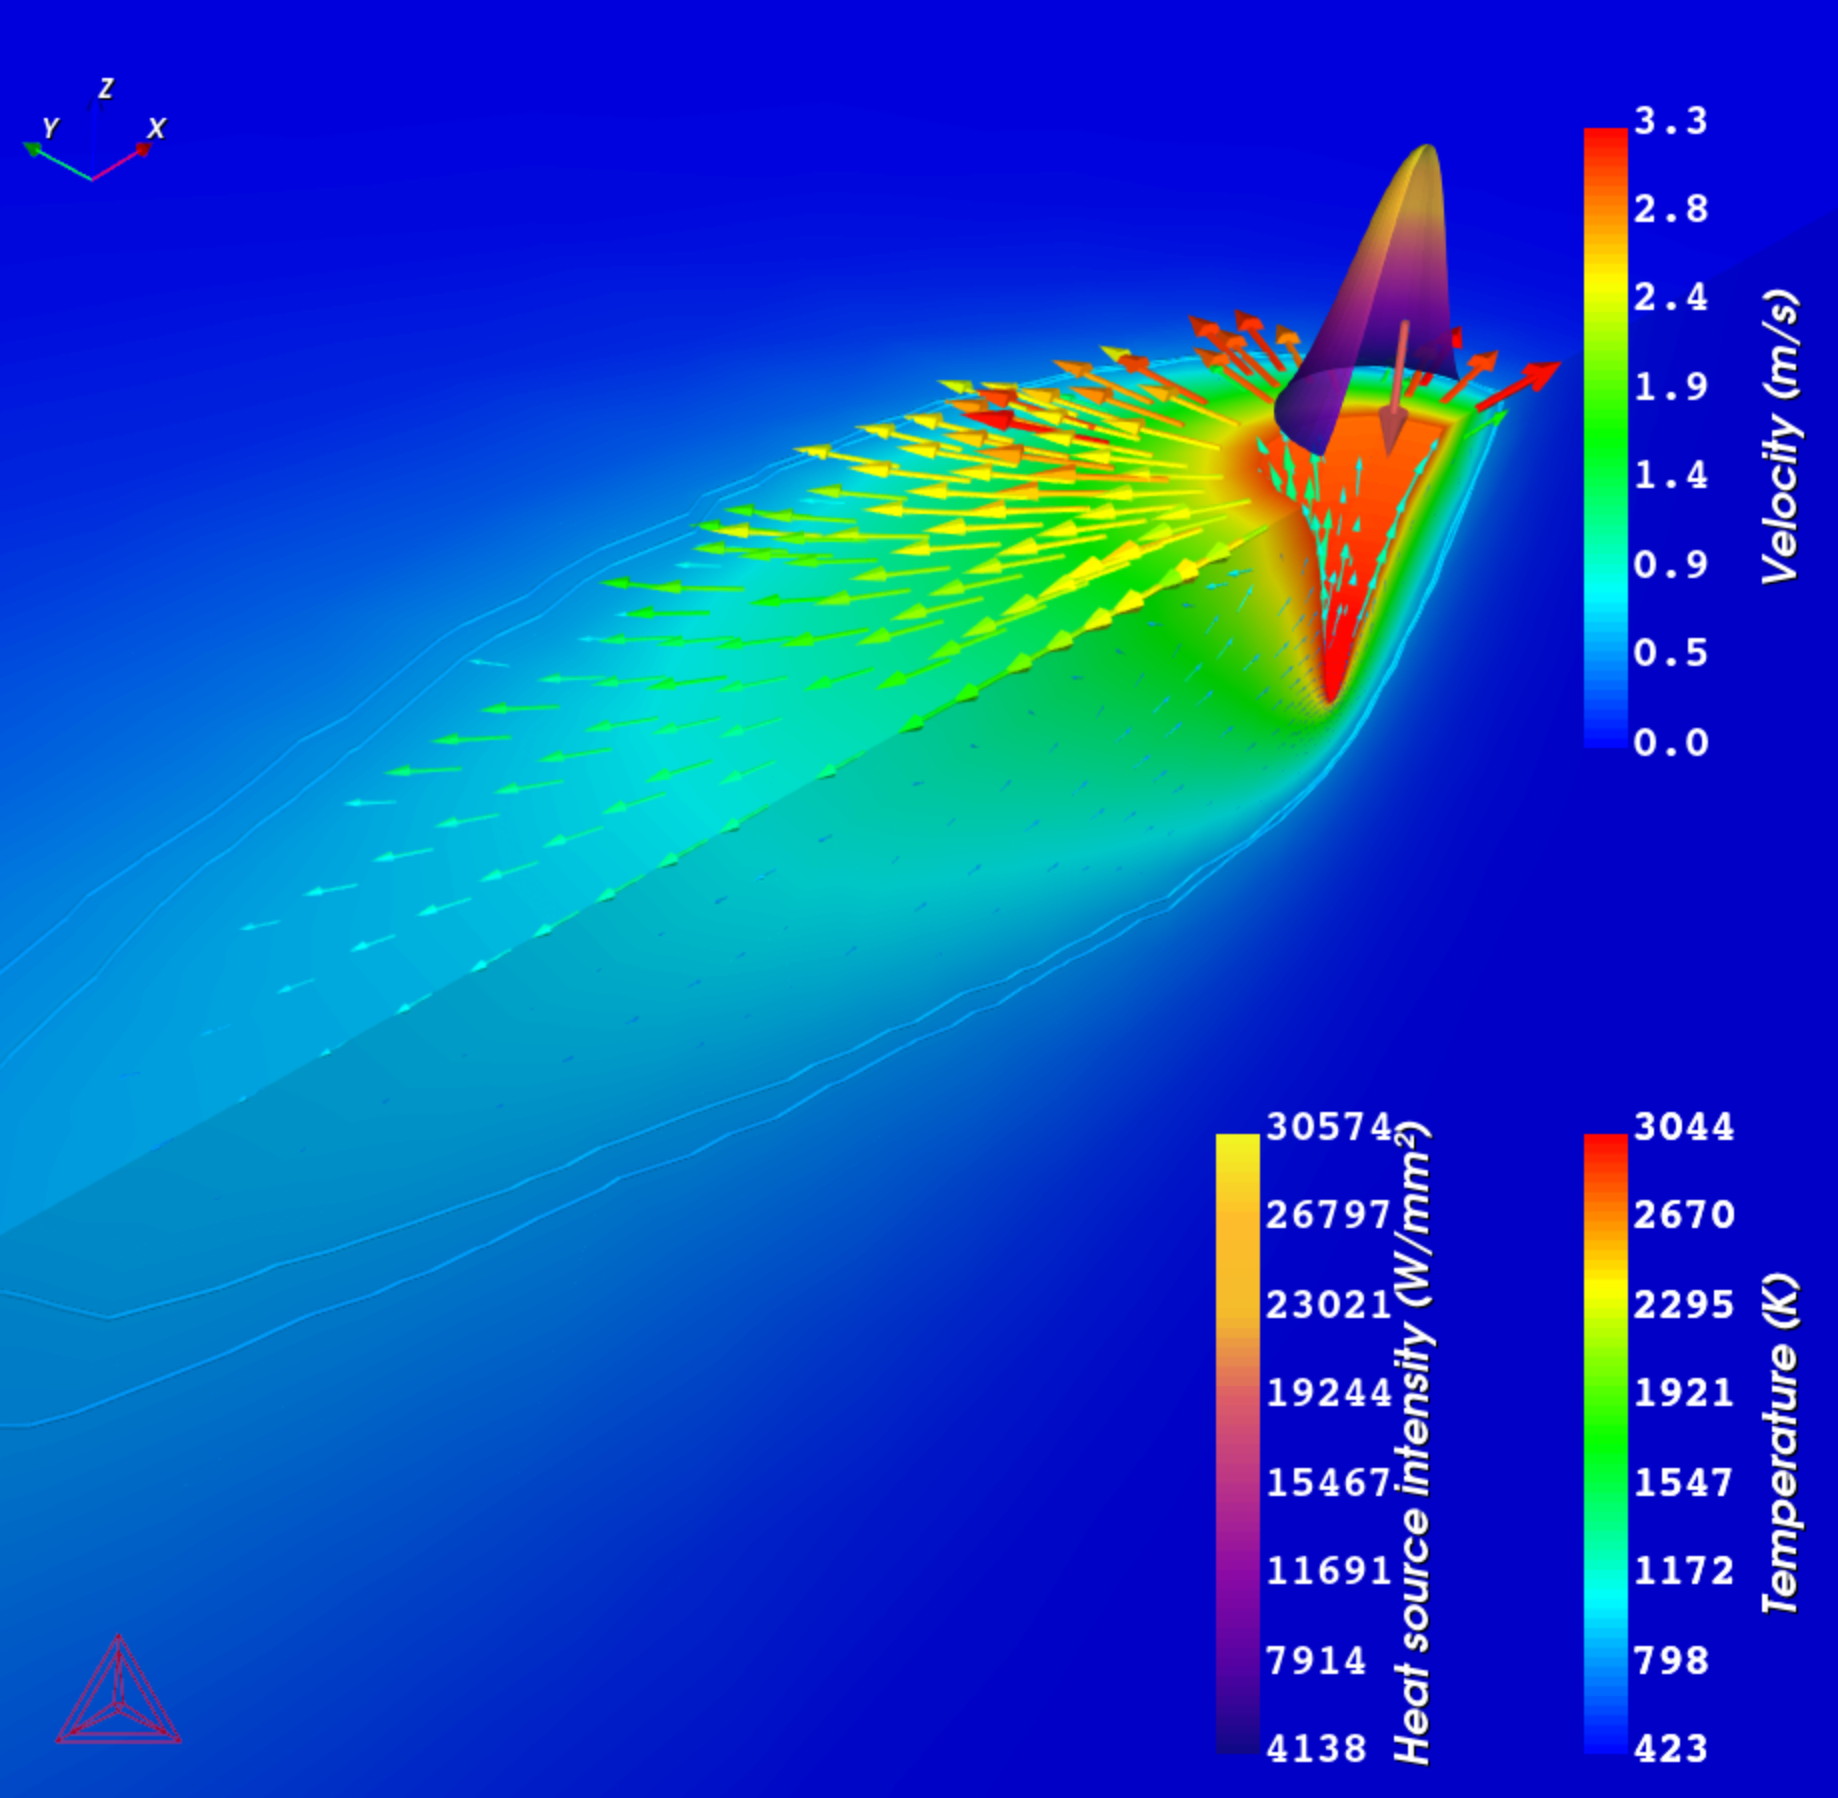
\includegraphics[width=0.42\linewidth,trim=2cm 1cm 2cm 1cm,clip]{../figures/thermo-calc-am-module-prelim-results/AlSi10Mg-meltpool-250W-900mms.png} &
    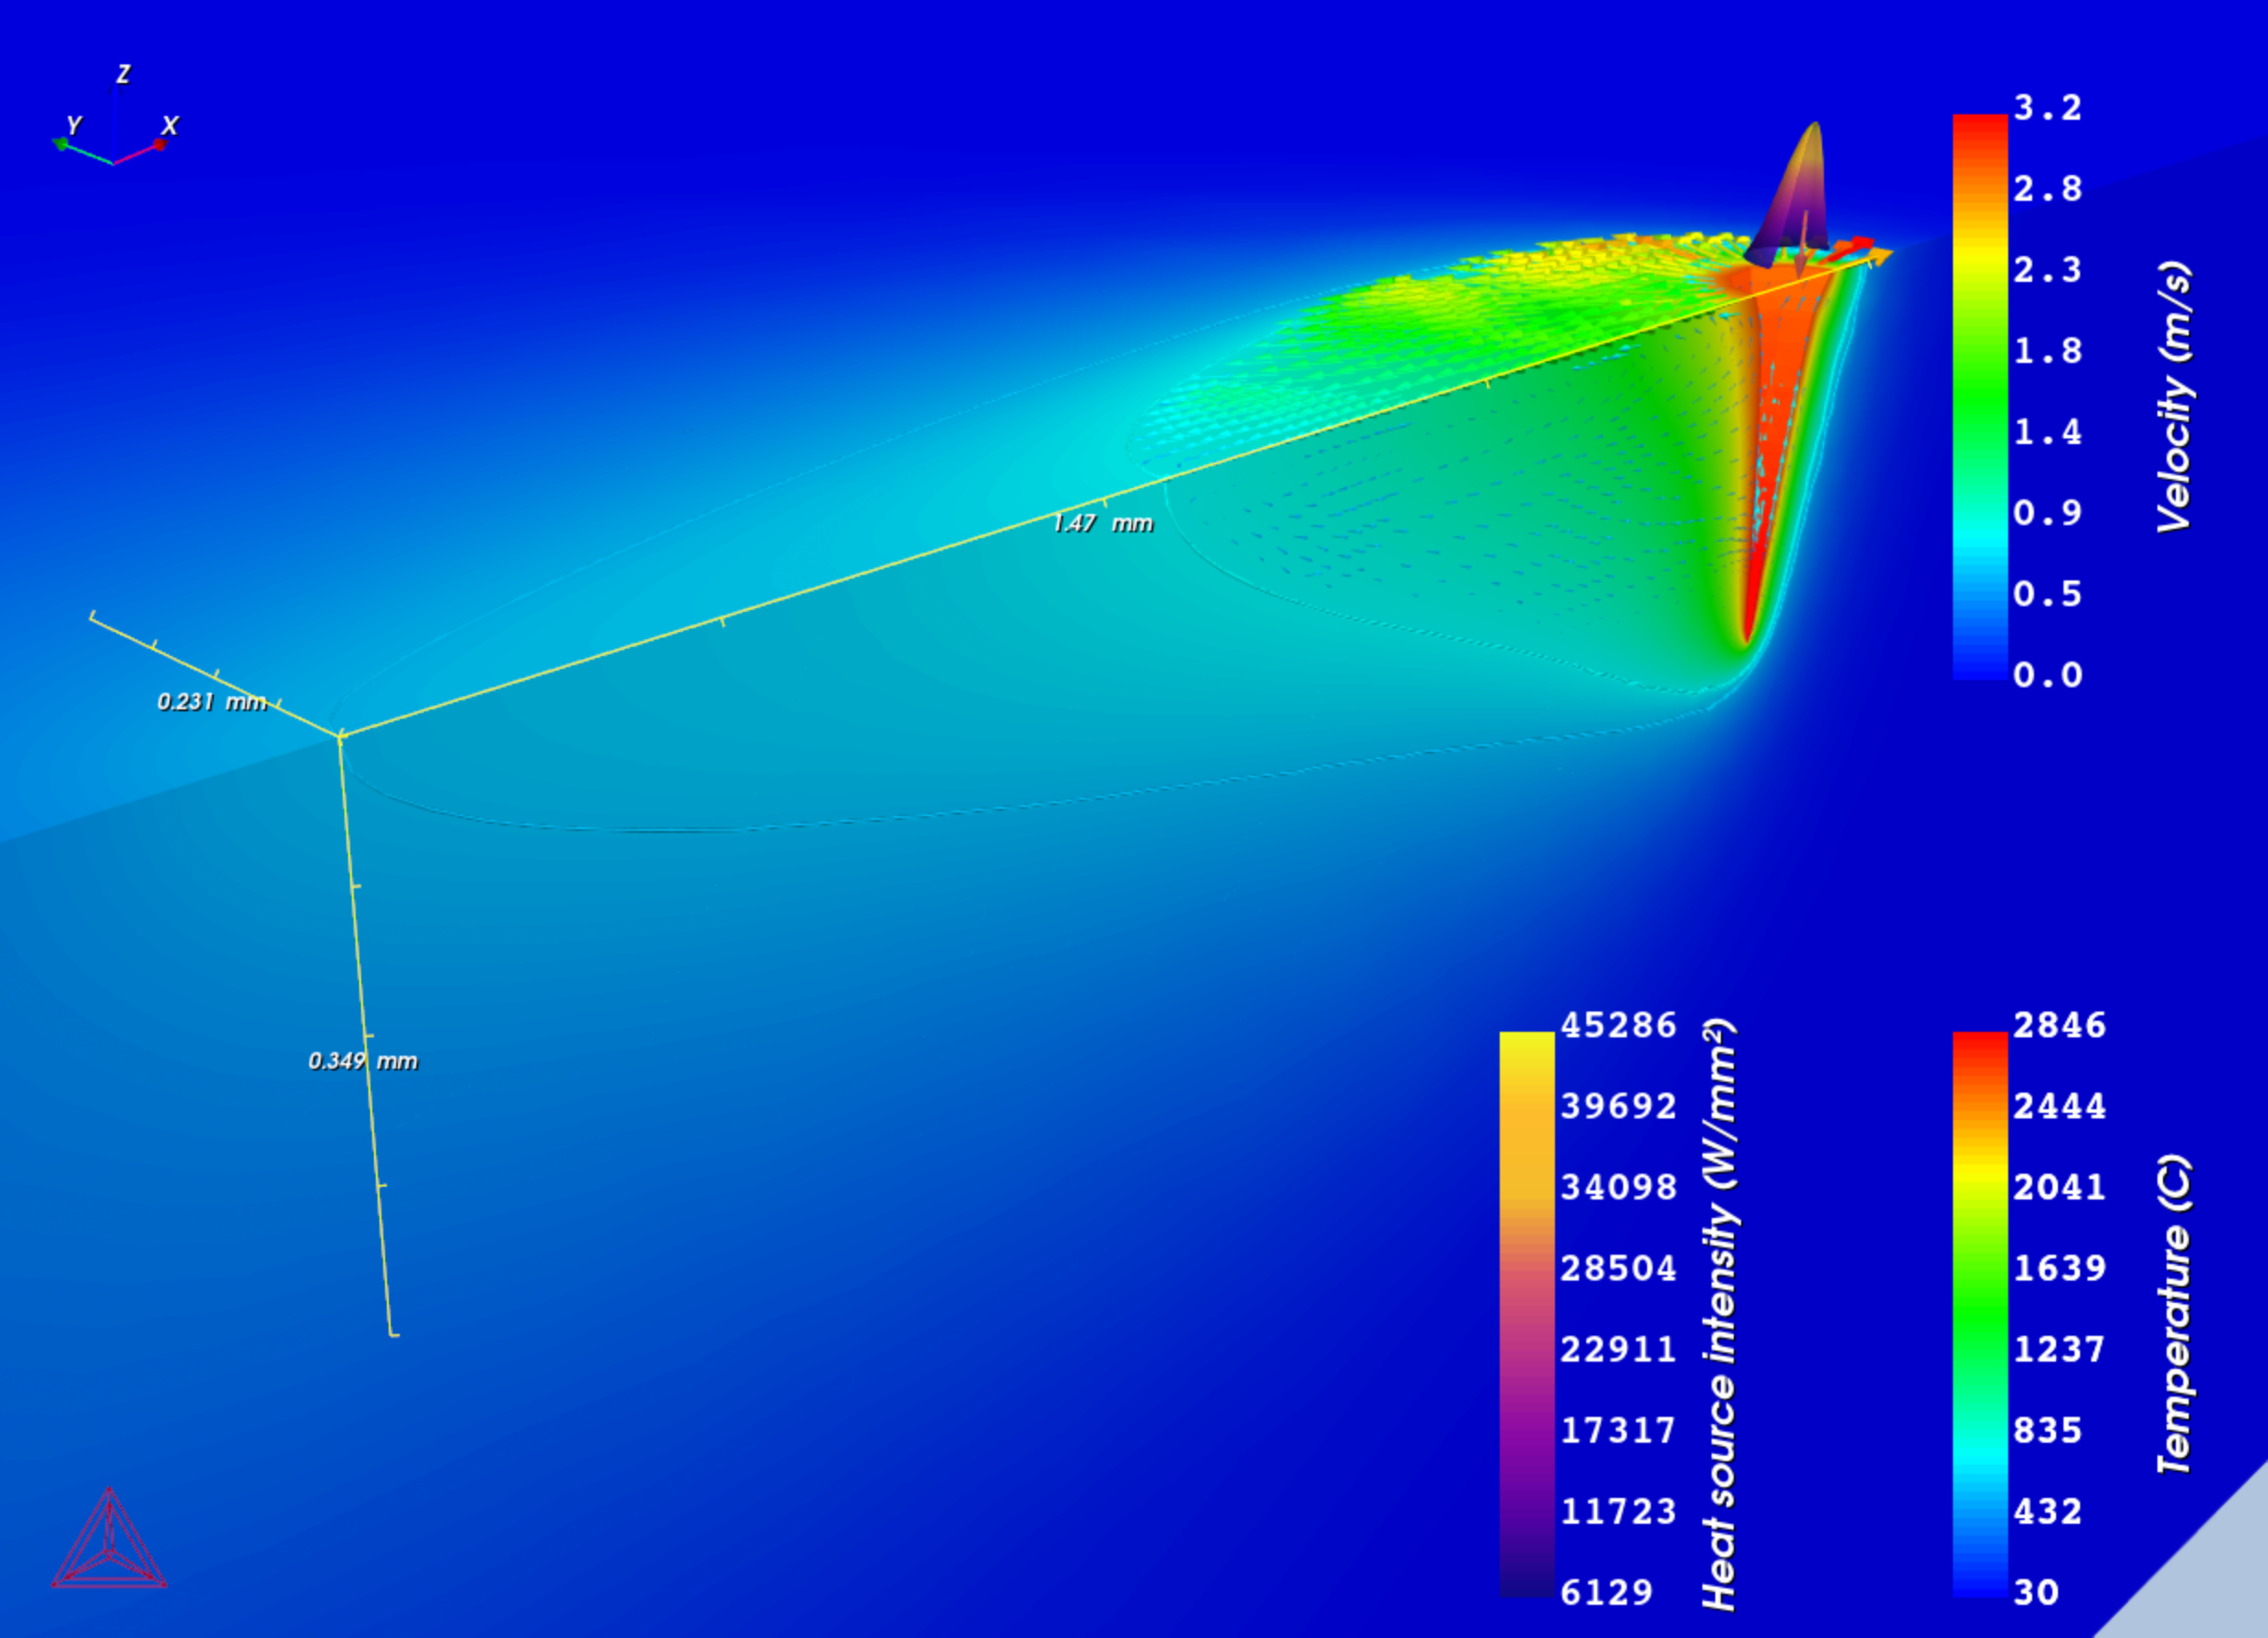
\includegraphics[width=0.42\linewidth,trim=2cm 1cm 2cm 1cm,clip]{../figures/thermo-calc-am-module-prelim-results/BYUMix-meltpool-375W-400mms.png} \\
    {\scriptsize (c) Stock AlSi10Mg melt pool, 250\,W / 900\,mm\,s$^{-1}$} & {\scriptsize (d) BYU blend melt pool, 375\,W / 400\,mm\,s$^{-1}$} \\
  \end{tabular}\\[6pt]
  \fbox{\begin{minipage}[c][1.0in][c]{0.5\linewidth}
    \centering\scriptsize
    \textit{Placeholder:} AMAZEMET-atomized AlSi10Mg+Si+Al-wire blend --- SEM + EDS maps.
  \end{minipage}}
  \caption{AlSi10Mg baseline sub-panels: (\textit{top}, a--d) Thermo-Calc AM~Module printability maps and steady-state melt-pool cross-sections for stock AlSi10Mg and the BYU AA1100+Si+AlSi10Mg blend planned for early FLAIME atomization (Thermo-Calc's account manager, preliminary results, M0). The two compositions bracket the upcoming FLAIME composition sweep and exercise the AM~Module's printability/melt-pool workflow before extension to the Al--Mn--Cr--Zr / Al--Zr anchor systems (Fig.~\ref{fig:anchor-calphad}). (\textit{bottom}) AMAZEMET-atomized AlSi10Mg+Si+Al-wire blend SEM + EDS maps (partner run in progress). Complements the SEM anchor figure in \S1 (Fig.~\ref{fig:baseline}).}
  \label{fig:baseline-supp}
\end{figure}

Sub-size ASTM~E8/E8M specimens (100\,mm length instead of 200\,mm) are
standard in LPBF screening with YS/UTS within
$\sim$5\%~\cite{paraschiv_2023_ma16144930,wang_2020_17452759};
elongation per ASTM~E8/E8M~\cite{astm_2024_e8e8m}.  The
atomize--print--density-gate pipeline success rate sets the upper bound
on compositions routed to tensile ($\sim$50--200) and
hardness/density ($\sim$150--450); preliminary AlSi10Mg tensile data
(Fig.~\ref{fig:tensile}) establishes the pipeline baseline before
campaign launch.  Elevated-temperature testing at three temperatures
validates L1$_{2}$ stability for DOE thermal applications with similar
or greater performance and lower critical mineral usage than the
incumbent Al--Zr.

\begin{figure}[!tb]
  \centering
  \fbox{\begin{minipage}[c][2.0in][c]{0.6\linewidth}
    \centering\scriptsize
    Placeholder:\\
    AlSi10Mg tensile curves + YS/UTS/EL bars
  \end{minipage}}
  \caption{AlSi10Mg preliminary tensile data (stress--strain, YS/UTS/EL; ASTM~E8, U.~Utah). Establishes pipeline baseline before FLAIME campaign launch.}
  \label{fig:tensile}
\end{figure}

\subsection*{A8.4 Mineral-Lean Baselines, Element Caps, and Per-Family Thresholds}
\label{app:a84-mineral-lean}

\textbf{Baselines (performance + mineral-lean).}
Al--Mn--Cr--Zr~\cite{thapliyal_2020_jmtla201} and Al--Zr (L1$_2$) serve as
\emph{performance} comparators for the BOFN surrogate. Because
Mn (100\% import-reliant), Zr (100\%), and Cr (74\%) are themselves
critical-mineral concerns, we add a second \emph{mineral-lean}
baseline family with the BO domain element-wise capped at
$\sum$(Mn,Cr,Zr) $\leq$ 1.0\,wt.\% (per-element caps:
\textbf{Mn $\leq$ 0.5\,wt.\%, Cr $\leq$ 0.3\,wt.\%, Zr $\leq$ 0.5\,wt.\%, Sc $\leq$ 0.05\,wt.\%}),
so the optimizer cannot recover Mn/Cr/Zr-heavy alloys with a different
trace dopant. Both baseline families are atomized early to seed the
surrogate. The discovery question is framed head-to-head: \emph{can
FLAIME recover X\% of the Al--Mn--Cr--Zr performance benchmark at
$\geq$50\% lower CMDRI mineral burden?} \textbf{G3b (CMDRI vs.\ AlSi10Mg)
is the primary discovery constraint with G3a (Sc-elimination)
retained as a screening floor}; literature parity on Al--Mn--Cr--Zr
validates the pipeline and flags systematic offsets before committing
the full campaign budget. pKGFN then routes evaluations across the
joint search space by cost-aware expected information gain. The G3a/G3b
framing is reported on a Pareto front of $\mathrm{CMDRI}_\text{log}$
vs.\ family-relative YS/EL, with the Pareto frontier itself (rather
than any single composition) as the primary Phase~I deliverable.

\textbf{Per-family performance thresholds.}
The family-specific mechanical targets referenced by Objective~O4 and
Table~\ref{tab:gates} are: \textbf{Al-Mn-Cr-Zr}---YS\,$\geq$\,250\,MPa,
EL\,$\geq$\,5\%; \textbf{Al-Zr}---YS\,$\geq$\,200\,MPa,
EL\,$\geq$\,8\%, with elevated-temperature retention. A Tier~1 pass
requires meeting both YS and EL for the relevant family on ASTM~E8
sub-size specimens with $\geq$3 replicates; the complementary
discovery metric is $\geq$20\% Tier~1 pass rate among $\geq$20 fully
tested compositions. Al-Mn-Cr-Zr and Al-Zr are the Phase~I
baseline comparators; thresholds for AI-discovered alloys outside
these families are set to the equivalent Scalmalloy-relative
performance band at Gate~G3 (see milestone M5/G3 in \S\ref{sec:milestones}).

\subsection*{A8.5 Comparative Landscape of SDL/BO Platforms for Structural AM}
\flaime{} is unique in unifying powder production, LPBF printing, and
tensile testing under a single AI decision loop with joint composition
and process optimization.  Related efforts fall short on one or more axes:
\textbf{APEX} envisions DED automation through hardness/compression
characterization but has been demonstrated only in a human-monitored
configuration with sparse implementation
detail~\cite{conn_2025_apex};
\textbf{A-Lab} targets oxides, not structural
metals~\cite{szymanski_2023_s4158602};
\textbf{AMASE} closes an experiment--theory loop on thin-film phase
maps, not bulk parts~\cite{liang_2025_sciadvad};
high-throughput \textbf{DED active-learning} platforms discover bulk
alloys at $>$100/week but use purchased feedstocks without LPBF or
tensile qualification~\cite{nelaturu_2024_jmsea202};
\textbf{BIRDSHOT} demonstrates closed-loop multi-objective BO with real
mechanical testing but on a pre-selected refractory system via arc
melting~\cite{paramore_2025_jactamat};
\textbf{ICME-anchored closed-loop Al for AM} has been demonstrated but
within expert-selected systems~\cite{thapliyal_2020_jmtla201}; and
recent \textbf{BO-guided CALPHAD} work optimizes within a single
expert-selected Al system using purely computational
objectives~\cite{glaser_2025_jmps106120}.
%%% END APPENDIX 8

% ============================================================================
%  SEPARATE FORMS (not included in the Field 8 PDF)
%  Excluded from final submission build; included in draft/clean for reference.
% ============================================================================
\ifsubmission\else
\newpage
\section*{\centering --- Separate Grants.gov Forms (Not in Field 8 PDF) ---}

\note{The following items are submitted via separate Grants.gov forms,
NOT inside the Project Narrative PDF.  They are included here for
drafting/planning reference only.}

% ========================= BUDGET ==========================================
\clearpage
\subsection*{SF-424 R\&R Budget Form + Budget Justification}
\label{sec:budget}

\instruct{The SF-424 Research \& Related (R\&R) Budget is the
standard Grants.gov budget form for federal research awards;
applicants complete it per-year (and cumulative) via the
Grants.gov Workspace.  See
\url{https://grants.gov/forms/r-r-family} for the form and
instructions.  The form itself lives outside this Field~8 PDF;
only the accompanying Budget Justification narrative is attached.
This Budget Justification is uploaded as a separate Grants.gov
attachment.}

\required{FOA \S IV.C: Budget on the SF-424 R\&R form. Budget
Justification attached to the budget form.  Use current negotiated
indirect cost and fringe benefit rates.  Justify all requested costs.}

\bigskip

\begin{center}
\textbf{\large Budget Justification}
\end{center}

\begin{quote}
\textit{\textbf{Compliant:} Totals balance to \textbf{\$600,000 BYU
portion} (at cap) and \textbf{\$743,999.99 total federal} (just under
the \$750,000 cap). Scope: capstones
+ validation network + Thermo-Calc + 4.5N argon, with elemental
feedstock right-sized to the 39-week PoP and the \$600K cap.}
\end{quote}

\textbf{Brigham Young University}

\subsubsection*{A. Senior/Key Personnel}

BYU faculty salary is calculated off an 8-month academic base. This
support is valuable in providing resources for dedicated faculty
support during the productive summer months.

\textbf{PI: Dr.\ Sterling Baird} --- Faculty summer support is requested
[per-person salary detail removed; included in the pooled personnel total].

\textbf{Fringe Benefits:} The 2026 fringe benefit rate for faculty
summer salary is 19.7\%. The total request for faculty summer wage
fringe benefits is included in the pooled personnel total [per-person fringe detail removed].

\subsubsection*{B. Other Personnel}

\textbf{Graduate Student Research Assistant:} Two full-time
(28~hours a week) graduate students will work throughout the
9~months of this project. The MS students will lead BOFN software
integration / data pipeline, experimental design and execution of
BOFN-guided campaigns, and experimental data ingest / CALPHAD
automation under PI supervision. [Per-person rate detail removed; included in the pooled personnel total.]

\textbf{Undergraduate Student Research Assistants:} 8~undergraduate
students will be hired hourly to work on this project. Students are
staggered across pipeline roles (atomization, LPBF handoff, SEM/EDS
characterization, tensile, data engineering) with intentional
redundancy for both safety and continuous coverage across terms.
Rates reflect BYU's undergraduate research pay scales for laboratory
work. [Per-person rate detail removed; included in the pooled personnel total.]

\textbf{Fringe Benefits:} No fringe rate applies to student salaries
during periods when students are enrolled in classes. No fringe
benefits are requested for students.

\subsubsection*{D. Travel}

\textbf{Validation:} Six trips are requested to various
collaborators to validate the printing. These trips will be taken
by students rather than by the PI, noting that not every
collaborator interaction will require BYU personnel on site.

\textbf{Valimet Coordination:} Three 3-day trips to Stockton,
California are requested for coordination with Valimet. Each trip
will include two BYU personnel and is timed with the three rounds
of gas atomization (two unique compositions per round, back-to-back).

\textbf{DOE Genesis Program Meeting:} One trip is requested for the
PI to attend the annual DOE Genesis Program Meeting.

\textbf{Conference:} Travel is requested for each of the two MS
students and the PI to attend one technical conference (TMS, MS\&T,
or MRS) to disseminate the results of the research.

Travel budget is requested for \textbf{\$1,300 per trip
(16~traveler-trips total). Total requested is \$20,800.}

\textit{Details Per Trip:}
\begin{itemize}\setlength{\itemsep}{0pt}
  \item Airfare: \$550
  \item Meals (per diem: \$74/day $\times$ 4~days): \$296
  \item Lodging (\$133 $\times$ 3~nights): \$399
  \item Ground Transportation: \$55
\end{itemize}
\textbf{Travel Total per Trip: \$1,300}

\subsubsection*{F. Other Direct Costs}

\textit{Materials and Supplies}
\begin{itemize}\setlength{\itemsep}{2pt}
\item \textbf{Research-scale elemental feedstock:} \$35,354 \\
sized from powder throughput and build geometry across both in-house
and partner LPBF systems. At BYU, builds are performed on the
\textbf{Mastrex MX-120} (120~mm diameter), co-located with the
ultrasonic atomizer (see letter of collaboration). At UofU, builds
are performed on the \textbf{Aconity MIDI} (170~mm diameter
$\times$ 200~mm height). Assuming $\sim$5~mm effective part height
and 3$\times$ hopper fill:
\begin{itemize}\setlength{\itemsep}{0pt}
  \item MX-120: area $\approx$113~cm$^2$ $\to$ part volume
  $\approx$56~cm$^3$ $\to$ powder $\approx$170~cm$^3$ $\to$
  $\approx$220~g/build (1.3~g/cm$^3$ apparent density
  ($\approx$1.6~g/cm$^3$ tap))
  \item Aconity MIDI: area $\approx$227~cm$^2$ $\to$ part volume
  $\approx$113~cm$^3$ $\to$ powder $\approx$340~cm$^3$ $\to$
  $\approx$440~g/build (1.3~g/cm$^3$ apparent density
  ($\approx$1.6~g/cm$^3$ tap))
\end{itemize}
Using a blended estimate ($\sim$300~g/build) over $\sim$320~builds
yields $\approx$96~kg powder demand; applying $\sim$2$\times$
factor for losses, recycling inefficiency, and failed prints gives
$\approx$190~kg total material demand. A substantial fraction of
the aluminum in each melt ($\approx$50--70\%) is provided by
\textbf{high-purity machined Al crucibles} (see separate line item
below), with the remainder supplied by elemental additions and
supplemental Al shot. Effective blended material cost
($\sim$\$150--\$200/kg) supports the request; adjusted for actual
39-week PoP (16~compositions/week $\times$ 39~weeks = 624 total
capacity).

\item \textbf{Gas-atomization feedstock (Valimet ingot material):}
\$25,000 \\
6~distinct ingot compositions $\times$ 500~lb each = 3,000~lb total;
\$3--\$10/lb range corresponds to \$9,000--\$30,000 total; \$25,000
used as a realistic midpoint for budgeting.

\item \textbf{Inert gas (4.5N-grade Ar, Ar-rich feed):} \$6,000 \\
per-run usage follows induction atomization workflow: multi-stage
purge ($\sim$400--500~L), process flow ($\sim$150~L), pour/boost
phase ($\sim$75~L), cooldown ($\sim$25~L) $\approx$650--750~L
Ar/run. Over $\sim$160 atomization runs (covering screened
compositions plus baseline, repeatability, and contingency runs),
this is $\sim$120~m$^3$ of Ar covered by $\sim$16 K-size 4.5N-Ar
cylinder exchanges at $\sim$\$210/exchange, plus cylinder rental
over 9~months on two on-site cylinders, and regulator/check-valve/
leak-test contingency.

\item \textbf{High-purity machined Al crucibles:} \$3,000 \\
machined in-house from 99.9--99.99\% Al bar stock; contributes
$\sim$50--70\% of melt mass per run and is explicitly accounted
for in feedstock totals. Cost reflects small-lot procurement and
machining scrap.

\item \textbf{Sonotrode tip replacement contingency:} \$2,500 \\
covers non-standard wear or damage during experimental campaigns
beyond nominal lifetime.

\item \textbf{LPBF consumables:} \$4,000 \\
build plates, recoater blades, filters, powder handling supplies,
sieves, and minor maintenance.

\item \textbf{UofU Metal 3D Printing Core Facility recharge:}
\$12,000 \\
$\approx$\$120/hr for $\sim$100 machine hours covering single
tracks, density cubes, and initial ASTM~E8 builds during
early-stage parameter development.

\item \textbf{Metallographic supplies:} \$3,000 \\
mounting resin, SiC paper, diamond paste, colloidal silica,
etchants.

\item \textbf{Characterization facility recharge fees:} \$22,000 \\
supports $\sim$320~compositions at $\sim$2~hr SEM/EDS + EBSD per
composition ($\sim$\$30/hr BYU subsidized rate), plus ICP-MS audits
($\sim$every 10th composition) and limited TEM validation on
high-performing alloys.

\item \textbf{ASTM E8/E8M tensile grips/fixtures:} \$3,000

\item \textbf{Safety / PPE and compliance:} \$8,368 \\
respirators, gloves, lab coats, safety training, hazmat disposal,
and gas handling infrastructure.

\item \textbf{Distributed validation network:} \$15,000 \\
cross-platform validation across LPBF/DED/binder jet partners;
$\sim$\$1,000/site average based on partner input.

\item \textbf{Thermo-Calc AB vendor procurement:} [amount removed] \\
TCAl10 + TCMG6 thermodynamic/kinetic database licenses, AM~Module
licensing, and dedicated technical-staff support including
TC-Python integration and AM~Module absorptivity calibration;
sole-source. MTDC-eligible vendor procurement, not a subaward.

\item \textbf{BYU Capstone Projects (2~teams):} \$44,000 \\
two senior capstone design teams.
\textbf{Team~A --- Lab Operations Toolkit (mechanical/manufacturing
focus):} designs operator-facing fixtures, safety-aligned workflows,
standard operating procedures, and a lightweight digital job-traveler
for powder production and handoff; $\sim$5--6 students.
\textbf{Team~B --- Research Data \& Sample-Tracking System (software/
systems focus):} develops web-based intake forms, sample-ID tracking
workflows, and dashboards linking powder batches, prints, and test
data into a unified data system; $\sim$5--7 students. Deliverables
include physical fixtures (Team~A) and a working web application and
data schema (Team~B). These teams provide structured, course-based
engineering effort supporting experimental operations, automation,
and data infrastructure.
\end{itemize}

\textbf{Total Supplies: \$208,222}

\textit{Research Publication Costs}

Open-access publication fees are requested to support dissemination
of Phase~I results in high-impact materials science and additive
manufacturing venues (e.g., \textit{Acta Materialia}, \textit{Additive
Manufacturing}, \textit{npj Computational Materials}). Typical article
processing charges (APCs) for these journals range from $\sim$\$1,500
to \$3,000 per article. The budget supports \textbf{two open-access
publications} to ensure rapid and broad dissemination of data,
methods, and discovered alloy systems, consistent with DOE and Genesis
Mission expectations for open science and FAIR data practices.
\textbf{Total requested is \$3,000.}

\textit{Graduate Student Tuition}

Graduate tuition is budgeted for all graduate students at BYU. Full
tuition for Fall~2026 and 3/4 tuition for Winter~2027
semesters is \$7,588 per student, consistent with current BYU
graduate tuition rates. Tuition support ensures sustained student
effort on research activities during the academic year without
competing teaching obligations. For 2~graduate students:
\textbf{\$15,176}.

\textit{Subaward to Valimet:} [amount removed] \\
Valimet's subaward request covers gas atomization of 6~distinct ingot
compositions (500~lb each) and associated coordination, with 

\subsubsection*{G. Total Direct Costs}

\textbf{\$407,657 (BYU-only direct, excludes the Valimet subaward)}

Breakdown: Personnel + Fringe (\$160,459) + Travel (\$20,800) +
Materials \& Supplies (\$208,222) + Research Publications (\$3,000)
+ Graduate Tuition (\$15,176) = \$407,657.

\subsubsection*{H. Indirect Costs}

F\&A is computed on Modified Total Direct Costs (MTDC) at BYU's
federally negotiated 51.5\% on-campus research rate.

\textbf{MTDC build-up:}
\begin{itemize}\setlength{\itemsep}{0pt}
  \item BYU-only direct: \$407,657
  \item + First \$25,000 of Valimet subaward (per 2~CFR \S200.1;
  the remainder of the subaward is excluded from
  MTDC): \textbf{+\$25,000}
  \item $-$ Graduate tuition remission (excluded from MTDC):
  \textbf{$-$\$15,176}
  \item $-$ BYU Capstone Projects (F\&A-exempt per BYU policy on
  course-based engineering effort): \textbf{$-$\$44,000}
  \item \textbf{MTDC base: \$373,481}
\end{itemize}

\textbf{F\&A:} 0.515 $\times$ \$373,481 = \textbf{\$192,343}\\
\textit{(Of this, \$12,875 = 0.515 $\times$ \$25,000 is the F\&A
charge on Valimet's first-\$25K MTDC entry; this \$12,875 is paid
out of the BYU portion because BYU is the prime.)}

\textbf{Total BYU (Direct + Indirect): \$600,000}

\subsubsection*{I. Total Amount Requested}

\textbf{\$743,999.99 total (BYU plus the Valimet subaward)}

\begin{quote}
\textit{Compliant with the \$600,000 BYU portion cap (at cap) and the
\$750,000 total federal cap (just under).}
\end{quote}

\note{PI ELIGIBILITY (FOA p.9--10): PI must be in a ``permanent or
indefinitely extensible position.''  Verify eligibility through
institutional sponsored programs office before submission.}

\note{ANNUAL MEETING TRAVEL (FOA p.57): ``Selected awardees will be
expected to attend up to two annual Genesis Mission meetings.''
Budget travel accordingly.}

\clearpage

% ========================= BIOSKETCHES ======================================
\subsection*{Biographical Sketches (SciENcv)}
\label{sec:biosketches}

\required{FOA \S IV.C: Attach via the Senior/Key Person Profile
(Expanded) form, NOT in the Project Narrative PDF.  Use SciENcv or
NSF-format biosketch.  \textbf{No page limit} for biosketches (FOA
p.118: ``there is no page limitation for the Biosketch, though some
fields in SciENcv have character limitations for consistency'').}

\instruct{Highlight: SDL publications, Bayesian optimization expertise,
materials informatics background, AM/alloy design experience,
qualification/standards work.}

% ---------- SciENcv Biographical Sketch: Sterling G. Baird ----------
% NOTE: Final version must be generated via SciENcv (ncbi.nlm.nih.gov/sciencv)
% and attached via the Senior/Key Person Profile (Expanded) form, NOT in this PDF.
% This LaTeX draft is for content preparation only.

\bigskip
\begin{center}
\textbf{Biographical Sketch --- Sterling G.\ Baird}
\end{center}

% --- Section A: Professional Preparation ---
\subsubsection*{A.\ Professional Preparation}

\begin{tabular}{@{}llll@{}}
\textbf{Institution} & \textbf{Major / Area} & \textbf{Degree} & \textbf{Year} \\[2pt]
Brigham Young University & Applied Physics & B.S. & 2018 \\
Brigham Young University & Mechanical Engineering & M.S. & 2021 \\
University of Utah & Materials Science \& Engineering & Ph.D. & 2023 \\
\end{tabular}

% --- Section B: Appointments and Positions ---
\subsubsection*{B.\ Appointments and Positions}

\begin{tabular}{@{}lp{8cm}@{}}
2025--present & Assistant Professor, Department of Mechanical Engineering,
                Brigham Young University \\[2pt]
2025          & Principal Investigator \& Staff Scientist,
                Acceleration Consortium, University of Toronto \\[2pt]
2024--2025    & Technical Consultant, Meta (Ax/BoTorch Bayesian
                Optimization Platform) \\[2pt]
2023--2025    & Director of Training and Programs,
                Acceleration Consortium, University of Toronto \\[2pt]
2020--2023    & Graduate Research Assistant (Sparks Group),
                University of Utah \\[2pt]
2017          & Research Intern, NASA Langley Research Center \\
\end{tabular}

% --- Section C: Products ---
\subsubsection*{C.\ Products (10 Most Relevant to Proposed Project)}

\begin{enumerate}[leftmargin=*]
\item G.\ Tom, S.\ P.\ Schmid, \textbf{S.\ G.\ Baird}, et al.,
  ``Self-Driving Laboratories for Chemistry and Materials Science,''
  \textit{Chemical Reviews} \textbf{124}(16), 9633--9732 (2024).
  DOI:~10.1021/acs.chemrev.4c00055

\item \textbf{S.\ G.\ Baird} and T.\ D.\ Sparks,
  ``What is a minimal working example for a self-driving laboratory?''
  \textit{Matter} \textbf{5}(12), 4170--4178 (2022).
  DOI:~10.1016/j.matt.2022.11.007

\item \textbf{S.\ G.\ Baird} and T.\ D.\ Sparks,
  ``Building a `Hello World' for self-driving labs: The Closed-loop
  Spectroscopy Lab Light-mixing demo,''
  \textit{STAR Protocols} \textbf{4}(2), 102329 (2023).
  DOI:~10.1016/j.xpro.2023.102329

\item \textbf{S.\ G.\ Baird}, J.\ R.\ Hall, and T.\ D.\ Sparks,
  ``Compactness matters: Improving Bayesian optimization efficiency of
  materials formulations through invariant search spaces,''
  \textit{Computational Materials Science} \textbf{224}, 112134 (2023).
  DOI:~10.1016/j.commatsci.2023.112134

\item \textbf{S.\ G.\ Baird}, M.\ Liu, and T.\ D.\ Sparks,
  ``High-dimensional Bayesian optimization of 23 hyperparameters over 100
  iterations for an attention-based network to predict materials property:
  A case study on CrabNet using Ax platform and SAASBO,''
  \textit{Computational Materials Science} \textbf{211}, 111505 (2022).
  DOI:~10.1016/j.commatsci.2022.111505

\item \textbf{S.\ G.\ Baird}, A.\ R.\ Falkowski, and T.\ D.\ Sparks,
  ``Honegumi: An interface for accelerating the adoption of Bayesian
  optimization in the experimental sciences,''
  \textit{arXiv preprint} arXiv:2502.06815 (2025). Under review.

\item S.\ Lo, \textbf{S.\ G.\ Baird}, J.\ Schrier, et al.,
  ``Review of low-cost self-driving laboratories in chemistry and materials
  science: The `frugal twin' concept,''
  \textit{Digital Discovery} \textbf{3}(5), 842--868 (2024).
  DOI:~10.1039/D3DD00223C

\item \textbf{S.\ G.\ Baird}, T.\ Q.\ Diep, and T.\ D.\ Sparks,
  ``DiSCoVeR: A Materials Discovery Screening Tool for High Performance,
  Unique Chemical Compositions,''
  \textit{Digital Discovery} (2022).
  DOI:~10.1039/D1DD00028D

\item \textbf{S.\ G.\ Baird}, M.\ Ansari, Z.\ Afzal, et al.,
  ``Bayesian Optimization Hackathon for Chemistry and Materials,''
  ChemRxiv (2025).
  DOI:~10.26434/chemrxiv-2025-dzh5z

\item \textbf{S.\ G.\ Baird}, H.\ M.\ Sayeed, J.\ Montoya, and T.\ D.\ Sparks,
  ``Matbench-genmetrics: A Python library for benchmarking crystal structure
  generative models using time-based splits of Materials Project structures,''
  \textit{Journal of Open Source Software} \textbf{9}(97), 5618 (2024).
  DOI:~10.21105/joss.05618
\end{enumerate}

% --- Section D: Synergistic Activities ---
\subsubsection*{D.\ Synergistic Activities}

\textbf{Sterling Baird}

\begin{enumerate}[leftmargin=*]
\item \textbf{Self-Driving Laboratory Leadership \& Community Building.}
  Guest Editor for \textit{npj Computational Materials} --- ``Self-Driving Labs
  for Chemistry and Materials Science'' collection (2024--present). Lead author
  of the structural materials section of a comprehensive \textit{Chemical
  Reviews} review on self-driving laboratories (Tom et al., 2024). Solo-organized
  the Acceleration Consortium Bayesian Optimization Hackathon (120 participants,
  62 organizations, 14 countries). Presented ``An Autonomous Vertical Cloud Lab
  for Additively Manufactured Aerospace Alloys'' at MRS Fall 2025.

\item \textbf{Open-Source Software \& Community Infrastructure.}
  Over 17,000 open-source code artifacts (15K commits, 1.5K issues, 913 pull
  requests) spanning materials informatics, Bayesian optimization, and laboratory
  automation. Developer of Honegumi (arXiv:2502.06815, 2025, under review)
  and xtal2png (JOSS, 2022).
  Technical Consultant to Meta for the v1.0 release of the Ax/BoTorch Bayesian
  optimization platform (Nov 2024--Jan 2025). Over 350 self-driving lab
  demonstration kits deployed worldwide.

\item \textbf{Training \& Workforce Development.}
  Delivered approximately 5,000 person-hours of self-driving laboratory training
  to roughly 700 individuals through workshops, microcredential courses, and
  hackathons. Built the Acceleration Consortium Development Lab from the ground
  up (\$600K in equipment, 500 line items, 24 months). Developed over 200 hours
  of course content in robotics, data science, and AI-driven experimental design.

\item \textbf{Standardization \& Open Science.}
  Principal Investigator on an NSF Pathways to Open-Source Ecosystems (POSE)
  project developing a community-governed materials informatics software
  toolchain. Contributing to Acceleration Consortium community standards for
  self-driving laboratory interoperability. Presenter at the German-Canadian
  Materials Acceleration Centre (GCMAC) Summer School (2024, 2025) and Review
  Panelist for the NSF TIP Directorate (2026).

\item \textbf{Open Data Impact \& Domain Expertise.}
  Creator of the Materials Project Time-Split (MPTS-52) benchmarking dataset,
  widely adopted in the crystal structure generative AI community (available as a
  Python package on PyPI), and developer of the Matbench-genmetrics
  framework (JOSS, 2024). Completed a \$34K industry research contract with
  Fehrmann Materials GmbH applying machine learning to joint strength and
  ductility prediction in aluminum alloys.
\end{enumerate}

\fi % end \ifsubmission\else (separate forms)
% ============================================================================
\end{document}
